\documentclass[12pt]{report}
\usepackage[utf8]{inputenc}
\usepackage{graphicx,wrapfig,lipsum}
\graphicspath{{Images/}}
\usepackage{array}
\usepackage{setspace}
\setstretch{1.5}
\usepackage{geometry}
\usepackage{hyperref}
\usepackage{multirow}
\hypersetup{
    colorlinks,
    citecolor=black,
    filecolor=black,
    linkcolor=black,
    urlcolor=black
}
\usepackage{dingbat}
\usepackage{listings}
\usepackage{acronym}
\geometry{a4paper, portrait, margin=30mm, bmargin=30mm, tmargin=30mm}
\usepackage{tikz,lipsum,lmodern}
\usepackage[most]{tcolorbox}
\usepackage{hyperref}
\usepackage{cite}
\usepackage{svg}
\usepackage{pdflscape}
\usepackage{adjustbox}
\usepackage{placeins}
\usepackage{booktabs}
\usepackage{xcolor}
\usepackage{colortbl}
\usepackage{array}
\usepackage{tikz}
\usetikzlibrary{positioning}
\usepackage{longtable}  % For tables that span multiple pages
% Define colors
\definecolor{headerblue}{RGB}{41, 65, 114}
\definecolor{lightgray}{RGB}{245, 245, 245}
\definecolor{mediumgray}{RGB}{230, 230, 230}

\newcommand\YAMLcolonstyle{\color{red}\mdseries}
\newcommand\YAMLkeystyle{\color{black}\bfseries}
\newcommand\YAMLvaluestyle{\color{blue}\mdseries}

\makeatletter

% here is a macro expanding to the name of the language
% (handy if you decide to change it further down the road)
\newcommand\language@yaml{yaml}

\expandafter\expandafter\expandafter\lstdefinelanguage
\expandafter{\language@yaml}
{
  keywords={true,false,null,y,n},
  keywordstyle=\color{darkgray}\bfseries,
  basicstyle=\YAMLkeystyle,                                 % assuming a key comes first
  sensitive=false,
  comment=[l]{\#},
  morecomment=[s]{/*}{*/},
  commentstyle=\color{purple}\ttfamily,
  stringstyle=\YAMLvaluestyle\ttfamily,
  moredelim=[l][\color{orange}]{\&},
  moredelim=[l][\color{magenta}]{*},
  moredelim=**[il][\YAMLcolonstyle{:}\YAMLvaluestyle]{:},   % switch to value style at :
  morestring=[b]',
  morestring=[b]",
  literate =    {---}{{\ProcessThreeDashes}}3
                {>}{{\textcolor{red}\textgreater}}1     
                {|}{{\textcolor{red}\textbar}}1 
                {\ -\ }{{\mdseries\ -\ }}3,
}
\newcommand\ProcessThreeDashes{\llap{\color{cyan}\mdseries-{-}-}}
\lstset{
    breaklines=true,
    basicstyle=\ttfamily\small,
    postbreak=\mbox{\textcolor{red}{$\hookrightarrow$}\space}
}

% switch to key style at EOL
\lst@AddToHook{EveryLine}{\ifx\lst@language\language@yaml\YAMLkeystyle\fi}
\makeatother
\begin{document}
\begin{center}
\thispagestyle{empty}
\LARGE{University of Applied Sciences Ulm}\\[-0.9ex]
\LARGE{Faculty of Electrical Engineering and Information Technology}\\[1ex]
\vspace{0.3cm}
\begin{center}

\includegraphics[width=7cm]{Images/Logo.png}\\
\vspace{0.9cm}
\textbf{\LARGE{Master Thesis}}
\medskip\par
\textbf{\normalsize{submitted for the degree of}} \\[1ex]
\textbf{\Large{Master of Engineering}}\\
\textbf{\normalsize{In System Engineering and Management}}\\
\vspace{0.5cm}
\large{A Concept and Implementation of a Proactive Asset Administration Shell with Multi-Agent System Integration using the Belief-Desire-Intention approach}\\[-1.5ex]
\bigskip\par
by \par
\large{Ahmed Ibrahim Almohamed, BEng}\\[-1ex]
\large{Matriculation Nr.: 6005151}\\ [-1ex]
\vspace{0.6cm}
\end{center}
\medskip
\end{center}
\begin{tabular}{ll}
  Submission Date:  & \today \\[-1ex]
  Supervisors: & Prof. Dr. Sven Völker \\[-1ex]
                & Prof. Dr.-Ing. Hartwig Baumgärtel \\
\end{tabular}


\newpage

\begin{abstract}

As industries move toward \ac{I4.0}, intelligent autonomous systems capable of managing physical assets are increasingly essential.
The \ac{AAS} has emerged as a key technology for standardizing the representation and management of digital twins.
Among AAS types, the \ac{Type3AAS} is distinguished by its capacity to encapsulate not only an asset's data and functions but also its proactivity.
This thesis proposes an approach to implementing \ac{Type3AAS} using \ac{MAS} based on the \ac{BDI} architecture.
A systems engineering approach was taken to define the requirements, concept, and implementation of the proposed solution.
The work establishes foundational submodels for the \ac{AAS} and demonstrates their application through a production resource use case involving drill machines.
The proof of concept is validated by the ability of the implemented \ac{Type3AAS} to autonomously manage and optimize drill machine operations in a simulated production environment.
This thesis provides groundwork for further research and development in this area.
\end{abstract}

\chapter*{List of Acronyms}
%\addcontentsline{toc}{chapter}{List of Acronyms}
\begin{acronym}[JADEX] % Give the longest label here so that the list is nicely aligned
\acro{AAS}{Asset Administration Shell}
\acro{Type3AAS}{Type 3 Asset Administration Shell}
\acro{BDI}{Belief-Desire-Intention}
\acro{IIoT}{Industrial Internet of Things}
\acro{I4.0}{Industry 4.0}
\acro{RAMI4.0}{Reference Architectural Model Industrie 4.0}
\acro{MAS}{Multi Agent system}
\acro{DT}{Digital Twin}
\acro{XML}{eXtensible Markup Language}
\acro{JSON}{JavaScript Object Notation}
\acro{RDF}{Resource Description Framework}
\acro{API}{Application Programming Interface}
\acro{CRUD}{Create, Read, Update, Delete}
\acro{SYNC}{Synchronous}
\acro{ASYNC}{Asynchronous}
\acro{LLC}{Low-Level Control}
\acro{HLC}{High-Level Control}
\acro{FAAAST}{Fraunhofer Advanced AAS Tools for Simplified Interoperability}
\acro{PLC}{Programmable Logic Controller}
\acro{ACL}{Agent Communication Language}
\acro{FIPA}{Foundation for Intelligent Physical Agents}
\acro{OPC UA}{Open Platform Communications Unified Architecture}
\acro{MQTT}{Message Queuing Telemetry Transport}
\acro{HTTP}{Hypertext Transfer Protocol}
\acro{REST}{Representational State Transfer}
\acro{XMPP}{Extensible Messaging and Presence Protocol}
\acro{JADE}{JAVA Agent Development Framework}
\acro{JADEX}{JADE eXtension}
\acro{SPADE}{Smart Python Agent Development Environment}
\acro{CPS}{Cyber Physical Systems}
\acro{IDTA}{Industrial Digital Twin Association}
\acro{ACL}{Agent Communication Language}
\end{acronym}

\newpage
\listoffigures
\lstlistoflistings
\listoftables
\newpage

\newpage
\tableofcontents
\newpage

\section{Introduction}
\begin{tcolorbox}[colback=blue!5!white,colframe=blue!75!black,
  title=About this chapter]
  This chapter introduces the fundamental concepts and motivations behind the development of Type3 Asset Administration Shells (AAS) and their integration with Multi-Agent Systems (MAS) using the Belief-Desire-Intention (BDI) approach. It outlines the significance of AAS in the context of Industry 4.0, highlighting their role in enhancing asset management and interoperability. 
  We also go over the other chapters of this thesis to give a brief overview of the content covered.
\end{tcolorbox}

\newpage
\chapter{Fundamentals and State of the Art}
\label{ch:literature}

\section{Asset Administration Shells(AAS)}
The \ac{AAS} is one of the central concepts in the principles of Industry 4.0, 
providing a methodology for designing and implementing the digital representation 
of manufacturing process components \cite{arm2021automated}.
This section explores the fundamental concepts of the \ac{AAS}, its structure, 
and its role in enabling interoperability within Industry 4.0 ecosystems.
This section cover the specifications in \cite{plattformi40_aas_part1_v3}, \cite{plattformI40_aas_part2} that are of relevance
to this thesis.

\subsection{Basic concept of AAS}

The \ac{AAS} is a standardized digital representation of an asset,
which can be a physical or virtual entity within an industrial environment.
It serves as a cornerstone for achieving interoperability and seamless communication
of the asset with other components in the Industry 4.0 ecosystem \cite{idta2023metamodel}.
Together with the asset it represents, the \ac{AAS} forms the so-called 
\ac{I4.0} Component (I4.0-Component), as illustrated in Figure~\ref{fig:i4component}.
The asset can be any physical or non-physical entity that has value for an organization, 
including production systems, equipment, machines, components, products, raw materials, 
business processes, software, documents, and even human personnel \cite{idta2023metamodel}.

\begin{figure}[ht]
    \centering
    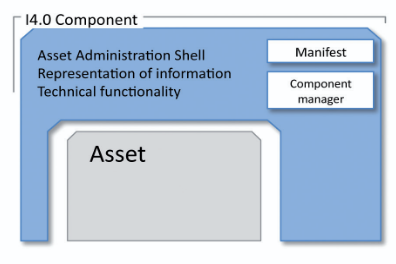
\includegraphics[width=10cm]{Images/AAS_OverViewConcept.png}
    \caption{The Industry 4.0 Component: Asset and its Administration Shell \cite{idta2023metamodel}}
    \label{fig:i4component}
\end{figure} 
At its core, the \ac{AAS} is an information model (meta model) that 
is exchanged between \ac{I4.0} components to enable interoperability \cite{plattformi40_aas_part1_v3}.
This information model could be represented as a \textit{\ac{XML}}, \textit{\ac{JSON}} or \textit{\ac{RDF}} document \cite{plattformi40_aas_part1_v3}.

The figure~\ref{fig:AAS_MetaModel} illustrates the meta model of the \ac{AAS},
which defines its structure and key components.
According to \cite{plattformi40_aas_part1_v3}, the \ac{AAS} has an \textit{Identifiable} attribute, which translate to an element
that is referable via a unique identifier.This attribute ensures that each \ac{AAS} can be distinctly identified within the Industry 4.0 ecosystem which also makes them unambiguous and easy to find.
Also it make the \ac{AAS} into an \textit{AdministrativeInformation} ,which contains information about the versioning , who created the last changes and information about the languages available in case the element contains text for translation \cite{plattformi40_aas_part1_v3}.
Also each \ac{AAS} has a \textit{HasDataSpecification} attribute, which means that it can be extended by using data specification templates , those define a named set of additional attributes that
an element may or shall have \cite{plattformi40_aas_part1_v3}.
The \ac{AAS} also has a \textit{derivedFrom} relation, which allows it to reference another \ac{AAS} from which it is derived.
This relation is useful for establishing hierarchies or relationships between different \ac{AAS}s.
The most important attribute of the \ac{AAS} is the \textit{HasSubmodel} attribute,
which indicates that the \ac{AAS} contains one or more submodels.
Submodels are modular components within the \ac{AAS} that encapsulate specific functionalities
and data related to the asset \cite{plattformi40_aas_part1_v3}.
Finally the \ac{AAS} has a \textit{AssetInformation} attribute, which provides essential meta data about the asset itself,
including the \textit{AssetKind}, which classify the asset into a \textit{Type AAS} or \textit{Instance AAS} \cite{plattformi40_aas_part1_v3}.
A \textit{Type AAS} represents a hardware or software element which specifies the common attributes shared
by all instances of the type \cite{plattformi40_aas_part1_v3}.
An \textit{Instance AAS} represents a specific occurrence of an asset,
which contains a concrete , clearly identifiable component of the type \cite{plattformi40_aas_part1_v3}.
The \textit{AssetInformation} attribute also includes the \textit{globalAssetId}, this attribute is required as soon as the AAS is
exchanged via partners in the life cycle of the asset.
In a first phase of the life cycle the asset might not yet
have a global ID but already an internal identifier. The
internal identifier would be modelled via\cite{plattformi40_aas_part1_v3}.

In summary, the \ac{AAS} provides a standardized framework for representing assets in a digital format,
enabling interoperability and seamless communication within Industry 4.0 environments.
Its meta model defines the structure and key components of the \ac{AAS},
laying the foundation for effective asset management and integration in modern industrial systems.

\begin{figure}[ht]
    \centering
    \includesvg[width=15cm,inkscapelatex=false]{Images/AAS_MetaModel.svg}
    \caption{Asset Administration Shell Meta Model \cite{plattformi40_aas_part1_v3}}
    \label{fig:AAS_MetaModel}
\end{figure}
\newpage

% ----------------------------------------------
\subsection{Submodels and data types}
A submodel is used to structure the digital representation and technical
functionality of an Administration Shell into distinguishable parts. Each submodel
refers to a well-defined domain or subject matter. Submodels can become
standardized and, thus, become submodels templates \cite{plattformi40_aas_part1_v3}.
In the figure~\ref{fig:Submodel_MetaModel}, the meta model of a submodel is illustrated.
Each submodel contains mainly \textit{submodel elements}, which are the building blocks of the submodel structure.
\textit{Submodel elements} can represent various types of data and functionalities,
including \textit{properties}, \textit{operations}, \textit{events}, and \textit{collections} etc.. \cite{plattformi40_aas_part1_v3}.
The Submodel also is an \textit{Identifiable} element, which means it has a unique identifier within the context of the \ac{AAS} \cite{plattformi40_aas_part1_v3}.
Similar to the \ac{AAS}, the Submodel also has an \textit{AdministrativeInformation} attribute,
which contains versioning and language information \cite{plattformi40_aas_part1_v3}.
Additionally, the Submodel has a \textit{HasDataSpecification} attribute, allowing it to be extended with data specification templates \cite{plattformi40_aas_part1_v3}.
This extensibility enables the inclusion of additional attributes and characteristics specific to the submodel's domain \cite{plattformi40_aas_part1_v3}.
The Submodel can also have a \textit{Qualifier} attribute, which provides additional context or metadata about the submodel element \cite{plattformi40_aas_part1_v3}.
Finally, the Submodel has a \textit{SemanticId} attribute, which links the submodel to a semantic definition,
enabling better understanding and interoperability of the submodel's content \cite{plattformi40_aas_part1_v3}.

\begin{figure}[ht]
    \centering
    \includesvg[width=15cm,inkscapelatex=false]{Images/Submodel_MetaModel.svg}
    \caption{Submodel Meta Model \cite{plattformi40_aas_part1_v3}}
    \label{fig:Submodel_MetaModel}
\end{figure}

The \textit{SubmodelElement} is the base element for all elements that can be part of a submodel.
The \textit{SubmodelElement} can be polymorphic, meaning it takes on different types as shown in figure~\ref{fig:SubmodelElement_MetaModel}.

\begin{landscape}
\begin{figure}[p]
    \centering
    \includesvg[width=20cm,inkscapelatex=false]{Images/SubmodelsElementsTypes_MetaModel.svg}
    \vspace{-5cm}
    \caption{Submodel Element Meta Model \cite{plattformi40_aas_part1_v3}}
    \label{fig:SubmodelElement_MetaModel}
\end{figure}
\end{landscape}
\newpage 

In table~\ref{tab:submodel_elements}, a brief description of the different types of \textit{SubmodelElements} is provided.

\definecolor{headerblue}{RGB}{41, 65, 114}
\definecolor{lightgray}{RGB}{245, 245, 245}

\begin{longtable}{>{\raggedright\bfseries}p{4.5cm} >{\raggedright}p{4.5cm} >{\raggedright\arraybackslash}p{4.5cm}}
\caption{Submodel Element Types and Definitions \cite{plattformi40_aas_part1_v3}} 
\label{tab:submodel_elements} \\

\toprule
\rowcolor{headerblue}
\textcolor{white}{Type} & \textcolor{white}{Definition} & \textcolor{white}{Specification} \\
\midrule
\endfirsthead

% Header for continuation pages
\multicolumn{3}{c}{\tablename\ \thetable{} -- continued from previous page} \\
\toprule
\rowcolor{headerblue}
\textcolor{white}{Type} & \textcolor{white}{Definition} & \textcolor{white}{Specification} \\
\midrule
\endhead

% Footer for pages that continue
\midrule
\multicolumn{3}{r}{\textit{Continued on next page}} \\
\endfoot

% Final footer
\bottomrule
\endlastfoot

% Table content
\rowcolor{lightgray}
Property & A data element with a simple value & valueType: DataTypeDefXsd [1..1] \\
Range & A data element with min and max values & min: ValueDataType [0..1], max: ValueDataType [0..1] \\
\rowcolor{lightgray}
Blob & Binary large object & value: BlobType [0..1], contentType: ContentType \\
File & Reference to an external file & value: PathType [0..1], contentType: ContentType \\
\rowcolor{lightgray}
ReferenceElement & Reference to another element & value: Reference [0..1] \\
Submodel\-Element\-Collection & A collection of submodel elements & value: SubmodelElement [0..*] \\
\rowcolor{lightgray}
Submodel\-Element\-List & An ordered list of submodel elements & value: SubmodelElement [0..*] \\
Entity & Represents an entity in a hierarchy & entityType: EntityType [1..1] \\
\rowcolor{lightgray}
Relationship\-Element & Defines a relationship between two elements & first: Reference, second: Reference \\
Annotated\-Relationship\-Element & Relationship with annotations & annotation: DataElement [0..*] \\
\rowcolor{lightgray}
Capability & Describes a capability of the asset & -- \\
Operation & Executable operation & inputVariable, outputVariable, inoutputVariable \\
\rowcolor{lightgray}
Basic\-Event\-Element & Describes an event & observed: Reference [1..1], direction: Direction \\
Multi\-Language\-Property & Property with multi-language support & value: LangStringSet [0..1] \\
\rowcolor{lightgray}
DataElement & Abstract base for data elements & (abstract class) \\

\end{longtable}
Along with the different types of \textit{SubmodelElements}, various \textit{data types} are used to define the values and attributes of these elements.
These \textit{data types} ensure consistency and standardization in representing information within the \ac{AAS} and shown in Figure~\ref{fig:data_types}.


\begin{figure}[ht]
    \centering
    \includesvg[width=12cm,inkscapelatex=false]{Images/DataTypes_MetaModel.svg}
    \caption{Data Types Meta Model \cite{plattformi40_aas_part1_v3}}
    \label{fig:data_types}
\end{figure}
Those \textit{data types} are divided into three main categories:
\begin{itemize}
    \item \textbf{decimalBuildInTypes}: These include basic data types such as \textit{string}, \textit{integer}, \textit{float}, \textit{boolean}, etc., which are used to represent simple values.
    \item \textbf{durationBuildInTypes}: These types are used to represent time durations and intervals, such as \textit{dayTimeDuration} and \textit{yearMonthDuration}.
    \item \textbf{PrimitiveTypes}: This category includes specialized data types like \textit{DateTime}, \textit{Date}, \textit{Time}, \textit{base64Binary}, etc., which provide more specific representations for certain kinds of data.
\end{itemize}

\subsection{Types of AAS}
The \ac{AAS} can be classified into three types based on the interaction between the \ac{AAS}s \cite{plattformI40_aas_part2}.
In Figure~\ref{fig:AAS_Types}, the three types of \ac{AAS} are illustrated.

The \textit{type1} \ac{AAS} represents a basic \ac{AAS} that is covered in previous sections, where those are simply 
file exchanges between \ac{I4.0} components.
The \textit{type2} \ac{AAS} introduces communication capabilities between \ac{AAS}s,where an \textit{\ac{API}} specification
is defined for that purpose \cite{plattformI40_aas_part2}.
The \textit{type2} \ac{AAS} allows for the active exchange of information and services between \ac{AAS}s,
enabling more dynamic interactions within the Industry 4.0 ecosystem on the contrary of 
\textit{type1} which is more passive \cite{plattformI40_aas_part2}.
The \textit{type3} \ac{AAS} builds on the capabilities of \textit{type2} and the 
specifications of \textit{type1} where it creates a peer-to-peer network of \ac{AAS}s 
which allows for a proactive exchange of the system \cite{plattformI40_aas_part2}.
According to \cite{plattformI40_aas_part2}, the \textit{type2} \ac{AAS}
has specification that are listed as in the table~\ref{tab:type2_specs}.

\begin{longtable}{>{\raggedright\bfseries}p{4.5cm} >{\raggedright}p{4.5cm} >{\raggedright\arraybackslash}p{4.5cm}}
\caption{Specification of \textit{type2 \ac{API}}\cite{plattformi40_aas_part1_v3}} 
\label{tab:type2_specs} \\
\toprule
\rowcolor{headerblue}
\textcolor{white}{Specification} & \textcolor{white}{Description} & \textcolor{white}{Reference} \\
\midrule
\endfirsthead 
% Header for continuation pages
\multicolumn{3}{c}{\tablename\ \thetable{} -- continued from previous page} \\
\toprule
\rowcolor{headerblue}
\textcolor{white}{Specification} & \textcolor{white}{Description} & \textcolor{white}{Reference} \\
\midrule
\endhead
% Footer for pages that continue
\midrule
\multicolumn{3}{r}{\textit{Continued on next page}} \\
\endfoot
% Final footer
\bottomrule
\endlastfoot
\ac{CRUD} AAS & create, read, update, delete \ac{AAS} & \cite{plattformi40_aas_part1_v3} \\
\rowcolor{lightgray}
\ac{CRUD} Submodels & create, read, update, delete submodels  & \cite{plattformi40_aas_part1_v3} \\
\ac{SYNC} Invokers & Invoke methods synchronously & \cite{plattformi40_aas_part1_v3} \\
\rowcolor{lightgray}
\ac{ASYNC} Invokers & Invoke methods asynchronously & \cite{plattformi40_aas_part1_v3} \\
Eventing  & subscribe and unsubscribe to events & \cite{plattformi40_aas_part1_v3} \\
\end{longtable}

\begin{figure}[ht]
    \centering
    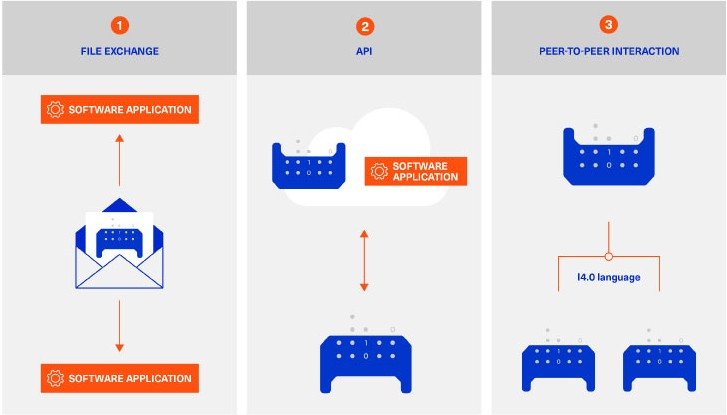
\includegraphics[width=12cm]{Images/AAS_Types.jpg}
    \caption{Types of Asset Administration Shells \cite{plattformI40_aas_part2}}
    \label{fig:AAS_Types}
\end{figure}

\newpage
\subsection{AAS Type3}
\label{subsec:aas_type3}
The \textit{type3} \ac{AAS} builds upon the capabilities of \textit{type2} \ac{AAS} by introducing a peer-to-peer network of \ac{AAS}s \cite{Sakurada2025_MAS_AAS_Type3}.
The \textit{type3} represents a more advanced and extended form of \ac{AAS}, 
acting as a decision-making entity that autonomously interacts with other \ac{AAS}s to exchange information and collaborate (e.g., through negotiation) \cite{Sakurada2025_MAS_AAS_Type3}.
The core idea of the Asset Administration Shell \ac{AAS} concept is that every industrial asset is represented by its own \ac{AAS}, 
thereby transforming the asset into an \ac{I4.0} component \cite{Sakurada2025_MAS_AAS_Type3}.
Because all \ac{AAS}s follow a unified, standardized structure and expose \ac{I4.0}-compliant interfaces, 
they enable seamless information provision and exchange across the entire lifecycle of an asset.
This standardization facilitates interoperability and real-time data sharing among heterogeneous assets, 
independent of manufacturer or application domain \cite{LOPEZ2023103859}.
In figure~\ref{fig:AAS_Type3_Concept}, the concept of \textit{type3} \ac{AAS} is illustrated.
\begin{figure}[ht]
    \centering
    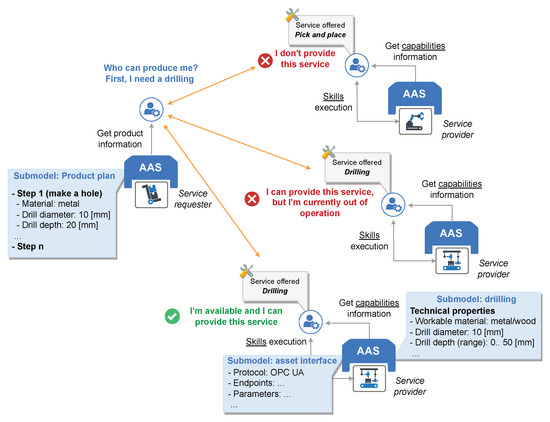
\includegraphics[width=12cm]{Images/type3_aas.jpg}
    \caption{Concept of Type3 AAS \cite{Sakurada2025_MAS_AAS_Type3}}
    \label{fig:AAS_Type3_Concept}
\end{figure}
Through their \ac{AAS} representations, assets are thus envisioned to autonomously collaborate, 
coordinate processes, and contribute to decentralized decision-making within industrial systems \cite{LOPEZ2023103859}.
However, such autonomous, intelligent, and cooperative behavior corresponds primarily to \ac{AAS} \textit{type3}, 
which unlike \ac{AAS} \textit{type1} and \textit{type2} remains comparatively underexplored and currently lacks dedicated specifications and comprehensive implementation guidelines \cite{Sakurada2025_MAS_AAS_Type3}.
The \textit{type3} \ac{AAS} revolves around three main requirements \cite{Sakurada2025_MAS_AAS_Type3} , \cite{LOPEZ2023103859}, \cite{vogel2021approach}, \cite{monostori2006agent}:
\begin{itemize}
    \item \textbf{Autonomy}: Each \ac{AAS} should operate independently, makin g decisions and executing actions without human intervention.
    \item \textbf{Intelligence}: \ac{AAS}s should possess cognitive capabilities, enabling them to learn from their environment, adapt to changes, and optimize their performance over time.
    \item \textbf{Collaboration}: \ac{AAS}s should be able to communicate and collaborate with other \ac{AAS}s, forming a network of interconnected agents that work together to achieve common goals.
\end{itemize}
The \textit{type3} is currently an area of active research and development,
with ongoing efforts to define its specifications and explore its potential applications in Industry 4.0 environments \cite{Sakurada2025_MAS_AAS_Type3}.
There is to be yet no standardized framework or guidelines for implementing \textit{type3} \ac{AAS},
making it a promising avenue for future exploration and innovation in the field of industrial automation and digitalization \cite{Sakurada2025_MAS_AAS_Type3}.

\subsection{Summary}
\label{subsec:aas_summary}

This section has introduced the \ac{AAS} as the standardized digital representation of industrial assets within the Industry 4.0 ecosystem. The key concepts covered include:

\begin{itemize}
    \item The \ac{AAS} meta-model, which defines the structure for representing assets through identifiable, self-describing information models that can be exchanged in \ac{XML}, \ac{JSON}, or \ac{RDF} formats.
    
    \item Submodels as modular components that encapsulate specific aspects of an asset, including properties, operations, events, and capabilities. Standardized submodel templates enable interoperability across different vendors and application domains.
    
    \item The classification of \ac{AAS} into three types based on their interaction capabilities: Type~1 (file exchange), Type~2 (API-based communication), and Type~3 (peer-to-peer proactive interaction).
    
    \item The requirements of \ac{Type3AAS}---autonomy, proactive behavior, and collaboration---which extend beyond the current specifications and require additional technologies to be realized.
\end{itemize}

Of particular relevance to this thesis is the \ac{Type3AAS}, which envisions assets as autonomous entities capable of proactive decision-making and peer-to-peer collaboration. However, as noted, the \ac{Type3AAS} currently lacks formal specifications and implementation guidelines. The standardized Operation element defined in the \ac{AAS} meta-model provides a potential interface for executing agent actions, yet this capability remains underutilized in existing implementations. The following sections introduce \ac{MAS} and the \ac{BDI} architecture as enabling technologies for realizing the proactive capabilities required by \ac{Type3AAS}.



%-------------------
\section{Multi-Agent Systems (MAS)}
\label{sec:mas}

The concept of autonomous agents and \ac{MAS} has emerged as a powerful paradigm for designing and implementing complex distributed systems that require autonomous behavior, coordination, and adaptability \cite{wooldridge2009introduction}. This section introduces the fundamental concepts of agents and \ac{MAS}, establishing the theoretical foundation for understanding their integration with \ac{AAS} to realize \ac{Type3AAS} capabilities.

\subsection{Agents and Their Properties}
\label{subsec:agents_properties}

An agent is commonly defined as ``a computer system that is situated in some environment, and that is capable of autonomous action in this environment in order to meet its design objectives'' \cite{wooldridge2009introduction}. Unlike conventional software components that execute predefined instructions in response to method calls, agents exhibit a higher degree of autonomy and environmental awareness.

According to \cite{wooldridge1995intelligent}, an intelligent agent possesses the following essential properties:

\begin{itemize}
    \item \textbf{Autonomy}: Agents operate without direct intervention from humans or other agents. They have control over their own actions and internal state, making independent decisions based on their goals and perceptions.
    
    \item \textbf{Reactivity}: Agents perceive their environment through sensors or data interfaces and respond in a timely manner to changes that occur in it. This enables agents to adapt to dynamic conditions.
    
    \item \textbf{Proactivity}: Beyond merely reacting to environmental changes, agents can exhibit goal-directed behavior by taking initiative. They can anticipate future states and act to achieve their objectives without external prompting.
    
    \item \textbf{Social Ability}: Agents can interact with other agents (and potentially humans) through some form of agent communication language to coordinate activities, negotiate, and cooperate toward shared or individual goals.
\end{itemize}

These properties distinguish agents from traditional software objects and make them particularly suitable for applications requiring autonomous decision-making and adaptive behavior, such as the proactive capabilities envisioned for \ac{Type3AAS}.

\subsection{Multi-Agent Systems}
\label{subsec:mas_definition}

A \ac{MAS} is a system composed of multiple interacting agents that work together within a shared environment \cite{wooldridge2009introduction}. Each agent in a \ac{MAS} has its own goals, capabilities, and knowledge, and the collective behavior of the system emerges from the interactions among individual agents.

\ac{MAS} offer several advantages over centralized systems \cite{leitao2016smart}:

\begin{itemize}
    \item \textbf{Decentralization}: There is no single point of control or failure. Each agent operates autonomously, making the system more robust and resilient to local failures.
    
    \item \textbf{Scalability}: New agents can be added to the system without requiring fundamental changes to existing agents, allowing the system to grow incrementally.
    
    \item \textbf{Flexibility}: Agents can dynamically reorganize and adapt their interactions in response to changing requirements or environmental conditions.
    
    \item \textbf{Modularity}: Each agent encapsulates specific functionality, promoting separation of concerns and facilitating maintenance and evolution of the system.
\end{itemize}

These characteristics align closely with the requirements of modern manufacturing systems, where flexibility, adaptability, and resilience are essential to cope with increasing product variety, shorter product lifecycles, and unpredictable disruptions \cite{leitao2016smart}.

\subsection{Agent Architectures}
\label{subsec:agent_architectures}

Agent architectures define the internal structure of agents and how they process perceptions to generate actions. Three main categories of agent architectures have been identified in the literature \cite{wooldridge2009introduction}:

\textbf{Reactive Architectures} implement a direct mapping from perceptions to actions without maintaining an internal model of the world. These architectures, such as the subsumption architecture proposed by Brooks \cite{brooks1986robust}, are computationally efficient and provide fast responses but lack the ability to reason about complex goals or plan ahead.

\textbf{Deliberative Architectures} maintain an explicit symbolic model of the world and use logical reasoning to determine appropriate actions. These architectures can handle complex planning tasks but may be computationally expensive and slow to respond to rapidly changing environments.

\textbf{Hybrid Architectures} combine reactive and deliberative components to balance responsiveness with reasoning capabilities. A typical hybrid architecture consists of multiple layers: a reactive layer for immediate responses, a deliberative layer for planning and reasoning, and a coordination layer that mediates between them. The \ac{BDI} architecture, discussed in Section \ref{sec:bdi}, represents a well-established hybrid approach that provides both reactive capabilities and goal-directed reasoning.

\subsection{Agent Communication}
\label{subsec:agent_communication}

Communication is fundamental to \ac{MAS}, enabling agents to share information, coordinate activities, and negotiate agreements. The \ac{FIPA} has established standards for agent communication that are widely adopted in industrial applications \cite{fipa2002acl}.

The FIPA \ac{ACL} defines a set of performatives (communicative acts) that specify the intended meaning of messages exchanged between agents. Common performatives include:

\begin{itemize}
    \item \texttt{INFORM}: Used to share information or beliefs with other agents
    \item \texttt{REQUEST}: Used to ask another agent to perform an action
    \item \texttt{PROPOSE}: Used to make a proposal during negotiation
    \item \texttt{ACCEPT-PROPOSAL} / \texttt{REJECT-PROPOSAL}: Used to respond to proposals
    \item \texttt{CFP} (Call for Proposals): Used to initiate a negotiation or auction
\end{itemize}

These standardized performatives enable interoperability between agents developed using different frameworks and facilitate the implementation of coordination protocols such as the Contract Net Protocol \cite{smith1980contract}, which is commonly used for task allocation in manufacturing systems.

\subsection{Agent Coordination and Cooperation}
\label{subsec:agent_coordination}

In \ac{MAS}, agents must coordinate their activities to achieve common goals and avoid conflicts. Several coordination mechanisms have been developed \cite{wooldridge2009introduction}:

\textbf{Contract Net Protocol}: A market-based mechanism where a manager agent announces a task, receives bids from contractor agents, and awards the contract to the most suitable bidder. This protocol is widely used in manufacturing for dynamic task allocation \cite{smith1980contract}.

\textbf{Auction-Based Coordination}: Agents participate in auctions to acquire resources or tasks. Different auction types (English, Dutch, sealed-bid) offer trade-offs between communication overhead and optimality of allocation.

\textbf{Negotiation}: Agents engage in a dialogue to reach mutually acceptable agreements. Negotiation is essential when agents have conflicting interests but need to cooperate for mutual benefit.

\textbf{Organizational Structures}: Agents can be organized into hierarchies, teams, or coalitions with defined roles and responsibilities. Organizational models such as Moise+ \cite{hubner2007moise} provide formal frameworks for specifying agent organizations.

\subsection{Industrial Agents}
\label{subsec:industrial_agents}

The application of agent technology in industrial settings has given rise to the concept of industrial agents, which are agents specifically designed for manufacturing and production environments \cite{leitao2016smart}. Industrial agents typically operate within a two-layered architecture as illustrated in Figure \ref{fig:industrial_agent_layers}:
\begin{figure}[ht]
    \centering
    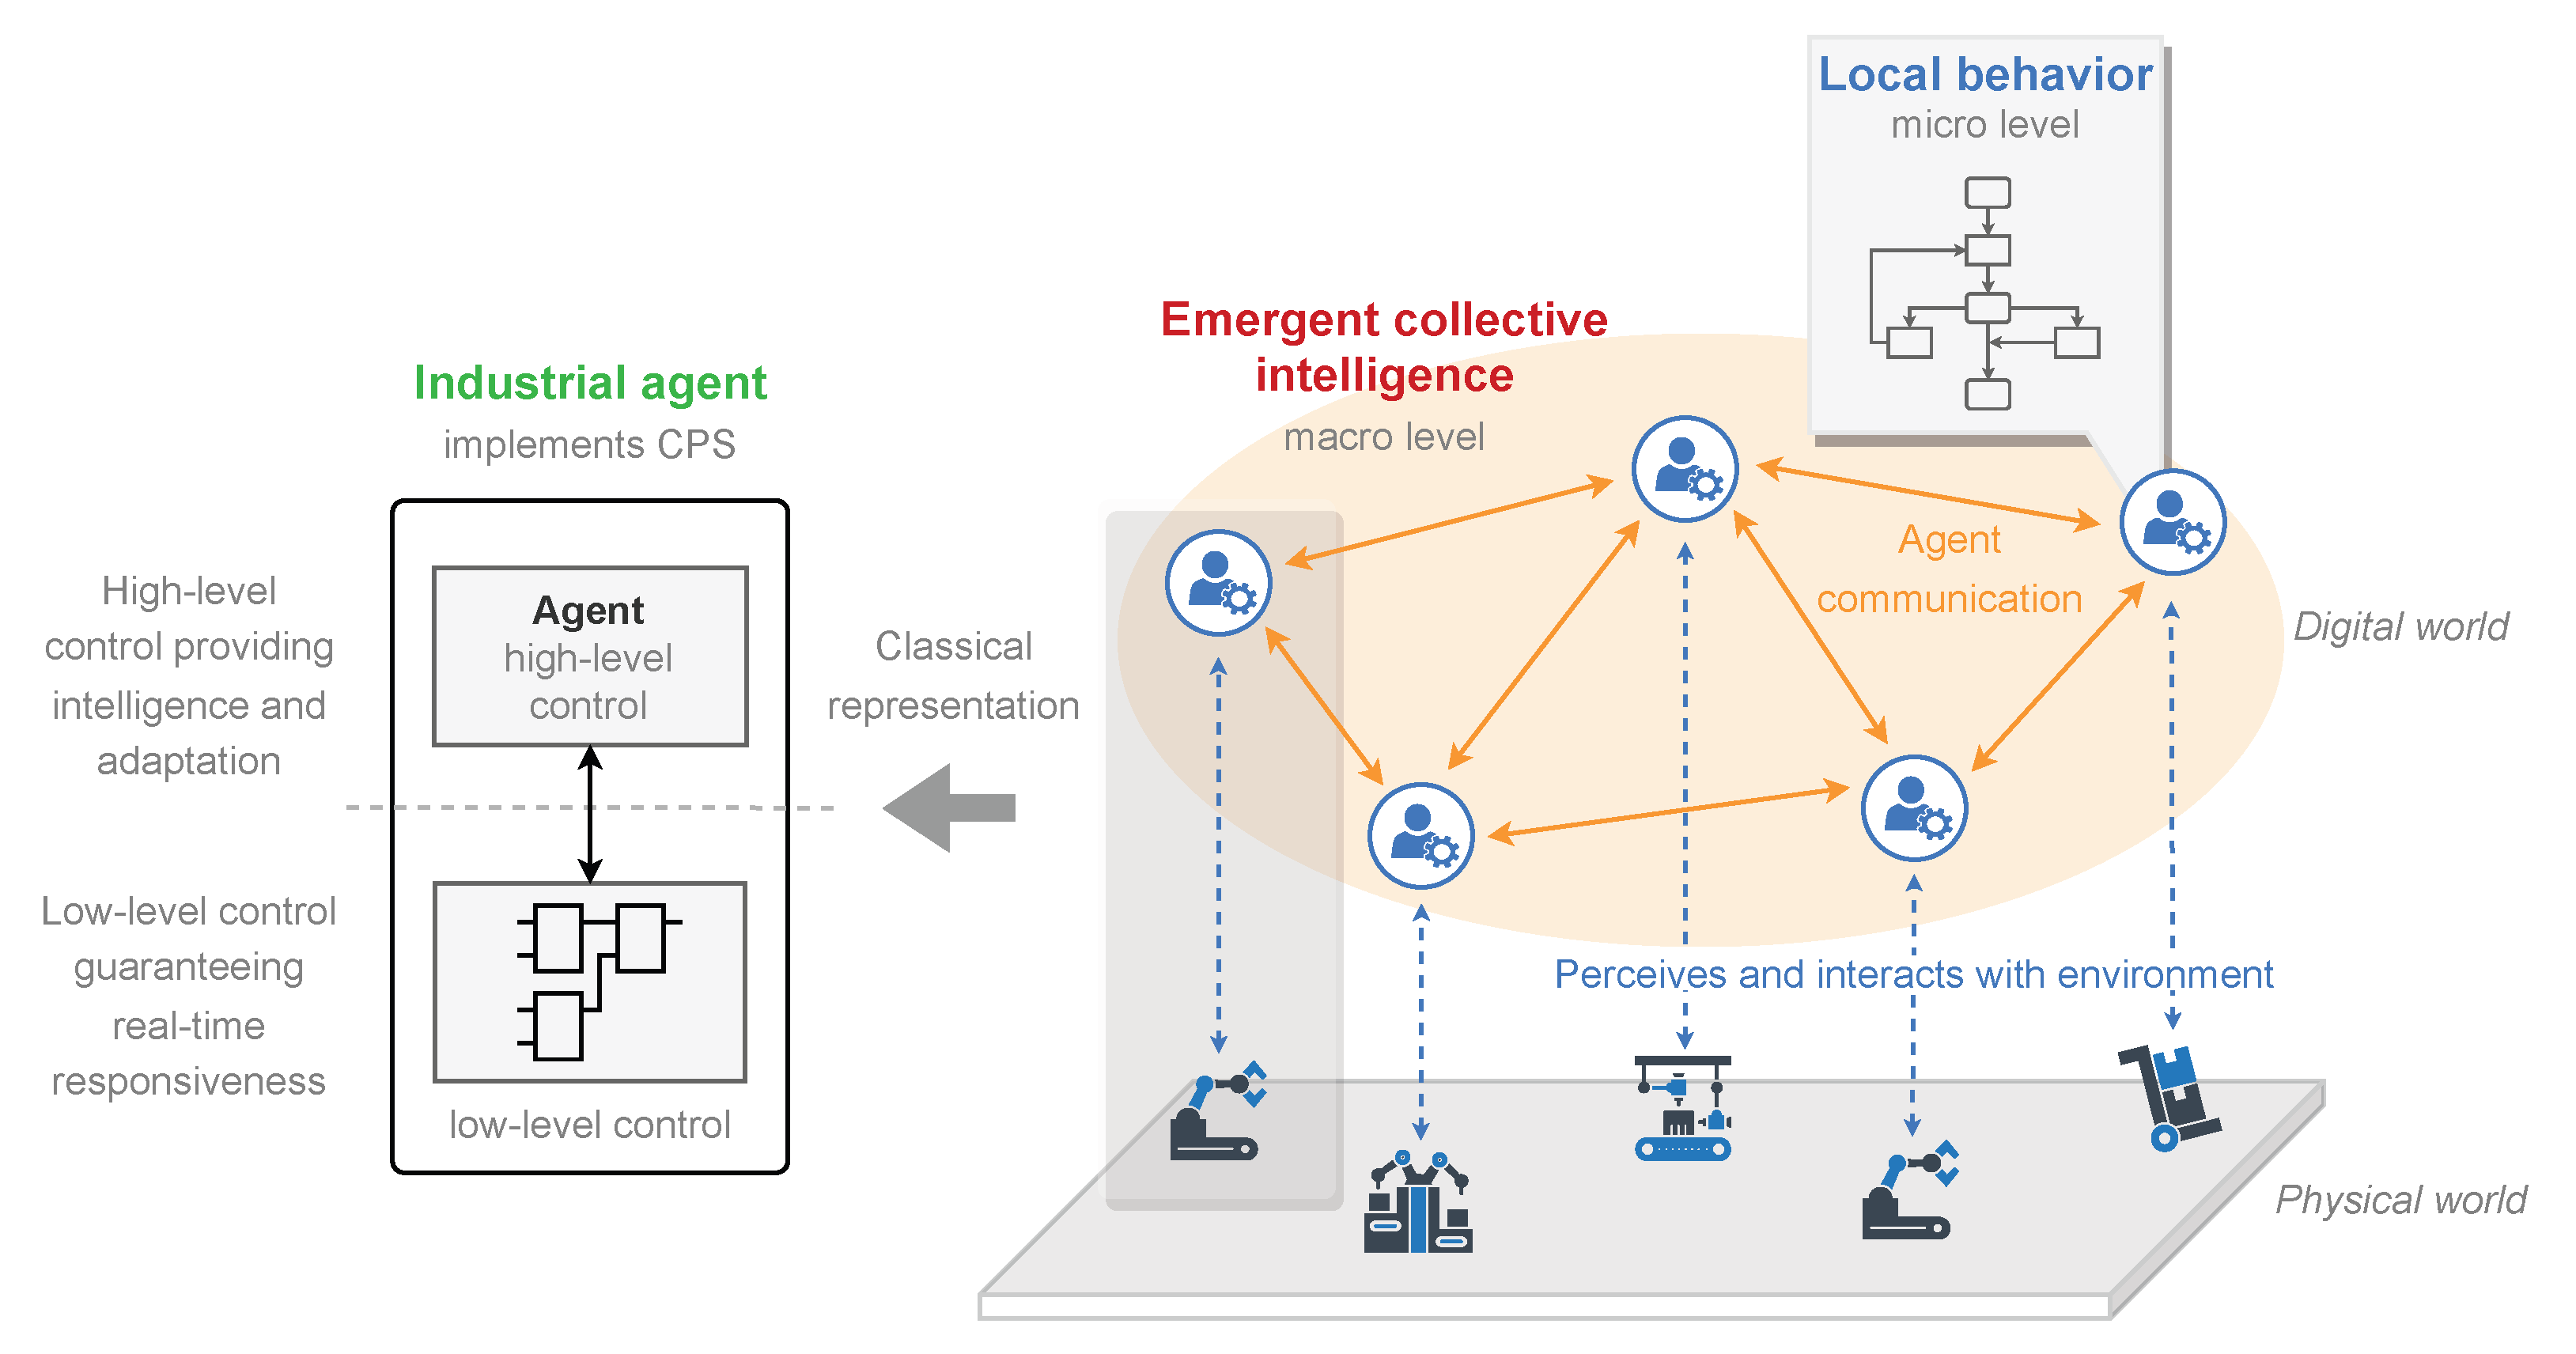
\includegraphics[width=12cm]{Images/Industrial_agent_approach.png}
    \caption{Industrial Agent Layers \cite{leitao2021recommendation}}
    \label{fig:industrial_agent_layers}
\end{figure}

\begin{itemize}
    \item \textbf{\ac{LLC}}: This layer handles real-time control of physical assets, including sensor monitoring, actuator control, and safety functions. It is typically implemented using \ac{PLC}s or industrial PCs with real-time operating systems.
    
    \item \textbf{\ac{HLC}}: This layer implements the agent logic, including decision-making, coordination, and communication with other agents. It provides intelligence and adaptability while delegating time-critical operations to the LLC layer.
\end{itemize}

This separation allows agents to leverage the reliability and determinism of industrial control systems while adding intelligent, adaptive behavior through the agent layer. The interface between these layers can be implemented using industrial communication standards such as \ac{OPC UA}, which aligns well with the communication capabilities specified for \ac{AAS} \cite{leitao2021recommendation}.

Industrial agents have been successfully applied in various manufacturing scenarios, including flexible manufacturing systems, supply chain management, and production scheduling \cite{leitao2016smart}. Their ability to operate autonomously, coordinate with peers, and adapt to changing conditions makes them natural candidates for implementing the proactive behavior required by \ac{Type3AAS}.

\subsection{Summary}
\label{subsec:mas_summary}

This section has introduced the fundamental concepts of agents and \ac{MAS}, including agent properties, architectures, communication, and coordination mechanisms. The key characteristics of agents autonomy, reactivity, proactivity, and social ability align directly with the requirements identified for \ac{Type3AAS}: autonomous operation, intelligent decision-making, and collaborative interaction. Industrial agents provide a proven approach for deploying agent technology in manufacturing environments, with established patterns for integrating intelligent behavior with real-time control systems. The following section examines the \ac{BDI} architecture, which provides a specific model for implementing rational, goal-directed agents suitable for \ac{Type3AAS} applications.



\newpage
\section{BDI (Belief-Desire-Intention) Approach}
\label{sec:bdi}
The \ac{BDI} architecture represents one of the most influential and well-established models for implementing rational agents capable of autonomous decision-making \cite{wooldridge1995intelligent}. Originally rooted in the philosophical theory of human practical reasoning developed by Bratman \cite{bratman1987intention}, the \ac{BDI} model has been successfully adapted into a computational framework for programming intelligent agents that exhibit goal-directed behavior \cite{rao1995bdi}.
\subsection{Foundations of the BDI Model}

The \ac{BDI} architecture is grounded in three core mental attitudes that guide an agent's reasoning and behavior \cite{bratman1987intention}:

\begin{itemize}
    \item \textbf{Beliefs}: Represent the agent's knowledge about itself, other agents, and its environment. Beliefs are informational states that the agent holds to be true based on its perceptions and prior knowledge. In the context of \ac{AAS}, beliefs can be derived from submodel data, sensor readings, or information received from other I4.0 components.
    
    \item \textbf{Desires}: Represent the goals or objectives that the agent would like to achieve. Desires are motivational states that drive the agent's behavior. For a \ac{Type3AAS}, desires might include optimizing production throughput, minimizing energy consumption, or completing manufacturing orders.
    
    \item \textbf{Intentions}: Represent the desires that the agent has committed to pursue. Intentions are deliberative states that the agent has decided to act upon, providing a form of commitment that ensures persistence in goal pursuit while allowing for reconsideration when circumstances change significantly.
\end{itemize}

The interplay between these three attitudes enables agents to reason about their goals, select appropriate plans, and execute actions in a rational manner \cite{rao1995bdi}. This separation of concerns allows for a clear distinction between what the agent knows (beliefs), what it wants to achieve (desires), and what it is currently trying to do (intentions).

\subsection{The BDI Reasoning Cycle}

A \ac{BDI} agent operates through a continuous reasoning cycle that processes perceptions from the environment and generates actions \cite{bordini2007programming}. The typical reasoning cycle consists of the following steps:

\begin{enumerate}
    \item \textbf{Perception}: The agent perceives changes in its environment and updates its belief base accordingly.
    
    \item \textbf{Belief Revision}: Based on new perceptions, the agent revises its beliefs to maintain consistency with the current state of the world.
    
    \item \textbf{Option Generation}: The agent generates possible options (potential desires) based on its current beliefs and existing goals.
    
    \item \textbf{Deliberation}: The agent deliberates over the available options and selects which goals to commit to as intentions.
    
    \item \textbf{Plan Selection}: For each intention, the agent selects an appropriate plan from its plan library that can achieve the intended goal given current beliefs.
    
    \item \textbf{Action Execution}: The agent executes the next action in the selected plan, which may affect the environment and trigger new perceptions.
\end{enumerate}

This cycle enables \ac{BDI} agents to exhibit both reactive behavior (responding to environmental changes) and proactive behavior (pursuing long-term goals), which aligns with the requirements of \ac{Type3AAS} \cite{wooldridge1995intelligent}.
\begin{figure}[ht]
    \centering
    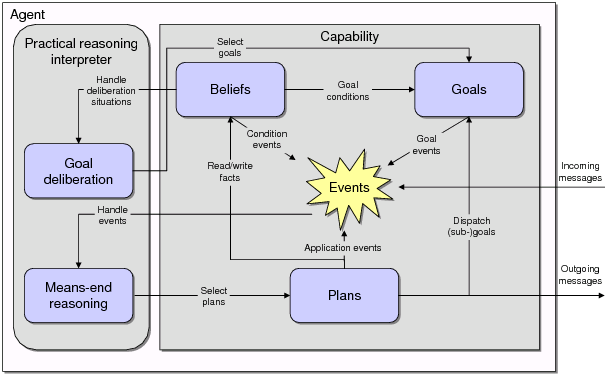
\includegraphics[width=12cm]{Images/BDI_concept.png}
    \caption{BDI Reasoning Cycle \cite{Pokahr2007_JadexConcepts}}
    \label{fig:bdi_reasoning_cycle}
\end{figure}

\newpage
\subsection{BDI for Industrial and Cyber-Physical Systems}

The application of \ac{BDI} agents in industrial settings has gained significant attention due to their ability to handle complex decision-making in dynamic environments \cite{leitao2021recommendation}. In the context of \ac{CPS} and Industry 4.0, \ac{BDI} agents offer several advantages:

\begin{itemize}
    \item \textbf{Autonomy}: \ac{BDI} agents can operate independently, making decisions without constant human supervision, which is essential for autonomous manufacturing systems.
    
    \item \textbf{Adaptability}: The belief revision mechanism allows agents to adapt to changing conditions in real-time, responding to unexpected events such as machine failures or order changes.
    
    \item \textbf{Explainability}: The explicit representation of beliefs, desires, and intentions provides a transparent model of agent behavior, facilitating debugging, validation, and trust in autonomous systems \cite{yan2025multi}.
    
    \item \textbf{Goal-Directed Behavior}: The intention-based commitment strategy ensures that agents persistently pursue their goals while maintaining the flexibility to reconsider when necessary.
\end{itemize}

\newpage

\subsection{Summary}

The \ac{BDI} architecture provides a well-founded theoretical and practical framework for implementing rational agents capable of autonomous decision-making. Its clear separation of beliefs, desires, and intentions enables transparent reasoning processes that are essential for industrial applications where explainability and trust are paramount. The availability of mature programming frameworks such as Jason and JaCaMo facilitates the development of \ac{BDI}-based multi-agent systems. When integrated with the \ac{AAS} concept, \ac{BDI} agents can leverage standardized asset information and communication interfaces to realize the proactive, collaborative behavior envisioned for \ac{Type3AAS}. This integration forms the conceptual basis for the approach proposed in this thesis.

\section{Software Frameworks and Platforms}
\label{sec:software frameworks and platforms}

The realization of \ac{Type3AAS} requires not only theoretical foundations but also practical software tools and frameworks. This section reviews the current state of available frameworks for implementing \ac{AAS}, \ac{MAS}, and \ac{BDI} agents, providing the technical context for the implementation decisions made in this thesis.



\subsection{Asset Administration Shell Frameworks}
\label{subsec:aas_frameworks}
Several open-source and commercial frameworks have emerged to support the development and deployment of \ac{AAS} implementations. The most prominent frameworks include:

\textbf{Eclipse BaSyx} is an open-source middleware platform developed under the Eclipse Foundation that provides a comprehensive implementation of the \ac{AAS} specification \cite{2023basyx}. BaSyx offers:
\begin{itemize}
    \item Complete implementation of the \ac{AAS} meta-model and API specification
    \item Support for both Type~1 (file-based) and Type~2 (API-based) \ac{AAS}
    \item Registry and discovery services for \ac{AAS} components
    \item Integration capabilities with industrial protocols (\ac{OPC UA}, \ac{MQTT}, \ac{HTTP},\ac{REST})
    \item Modular architecture allowing selective deployment of components
\end{itemize}
BaSyx is widely adopted in research and industry due to its open-source nature and active community support. However, it does not natively support \ac{Type3AAS} capabilities such as autonomous decision-making or proactive behavior.

\textbf{\ac{FAAAST}} is another open-source framework that focuses on ease of use and rapid prototyping \cite{2023faast}. It provides:
\begin{itemize}
    \item Lightweight implementation suitable for resource-constrained environments
    \item Support for multiple serialization formats (JSON, XML, RDF)
    \item Built-in synchronization with asset data sources
    \item Extensible architecture for custom functionality
\end{itemize}

\textbf{AASX Package Explorer} is a desktop application developed by the \ac{IDTA} for creating, viewing, and editing \ac{AAS} packages \cite{2023aasxexplorer}. While primarily a development and visualization tool rather than a runtime framework, it serves as an important reference implementation and is commonly used for:
\begin{itemize}
    \item Creating and validating \ac{AAS} models
    \item Importing and exporting \ac{AAS} packages in standardized formats
    \item Visualizing submodel structures and relationships
    \item Testing interoperability between different \ac{AAS} implementations
\end{itemize}

\textbf{Limitations for Type~3 AAS}: All current \ac{AAS} frameworks focus on Type~1 and Type~2 functionality. None provide native support for the autonomous, proactive behavior required by \ac{Type3AAS}. This gap motivates the integration with agent-based technologies explored in this thesis.


\subsection{Multi-Agent System Frameworks}
\label{subsec:mas_frameworks}

Several mature frameworks exist for developing \ac{MAS}, each with different design philosophies and target applications:

\textbf{\ac{JADE}} is one of the most widely used \ac{MAS} platforms, providing a FIPA-compliant infrastructure for agent development in Java \cite{2023jade}. Key features include:
\begin{itemize}
    \item Full compliance with \ac{FIPA} specifications for agent communication
    \item Distributed agent platform with support for multiple containers
    \item Built-in agent management and directory services
    \item Graphical tools for debugging and monitoring agent behavior
    \item Behavior-based agent programming model
\end{itemize}
\ac{JADE} has been extensively used in industrial applications and research projects. However, its behavior-based programming model does not directly support cognitive agent architectures such as \ac{BDI}.

\textbf{\ac{SPADE}} is a modern \ac{MAS} platform built on Python and \ac{XMPP} \cite{2023spade}. SPADE offers:
\begin{itemize}
    \item Asynchronous agent execution using Python's asyncio
    \item \ac{XMPP}-based communication providing robust, scalable messaging
    \item Web-based interface for agent monitoring
    \item Flexible behavior system with support for cyclic, one-shot, and finite-state behaviors
    \item Easy integration with Python's extensive ecosystem of libraries
\end{itemize}
\ac{SPADE}'s use of \ac{XMPP} provides advantages for industrial deployments, including message persistence, presence detection, and established security mechanisms. Its Python foundation also facilitates rapid prototyping and integration with data science tools.

\textbf{\ac{JADEX}} extends JADE with \ac{BDI} reasoning capabilities, combining JADE's robust infrastructure with cognitive agent programming \cite{2023jadex}. JADEX supports:
\begin{itemize}
    \item \ac{BDI} agent development using \ac{XML}-based agent definitions
    \item Integration with JADE's communication infrastructure
    \item Goal-oriented programming with automatic plan selection
    \item Active components model for service-oriented architectures
\end{itemize}

\subsection{Framework selection considerations}
The selection of appropriate frameworks for implementing \ac{Type3AAS} depends on several factors:

\begin{itemize}
    \item \textbf{AAS Compliance}: The \ac{AAS} framework must support the current specification, including submodel operations and standardized APIs.
    
    \item \textbf{Agent Architecture Support}: For \ac{BDI}-based implementations, the \ac{MAS} framework should either natively support \ac{BDI} or allow integration with \ac{BDI} reasoning engines.
    
    \item \textbf{Communication Capabilities}: Industrial deployments require robust, scalable communication mechanisms that can handle asynchronous messaging and potential network disruptions.
    
    \item \textbf{Integration Flexibility}: The ability to connect \ac{AAS} and \ac{MAS} components through well-defined interfaces is essential for realizing bidirectional integration.
    
    \item \textbf{Development Ecosystem}: Practical considerations such as documentation quality, community support, and available tooling influence development efficiency.
\end{itemize}

Tables~\ref{tab:aas_framework_comparison},\ref{tab:mas_framework_comparison} provides a comparative overview of the discussed frameworks.

\begin{table}[ht]
\centering
\caption{Comparison of Asset Administration Shell frameworks}
\label{tab:aas_framework_comparison}
\begin{tabular}{>{\raggedright}p{3.5cm} >{\centering}p{2.5cm} >{\centering}p{3cm} >{\centering\arraybackslash}p{4cm}}
\toprule
\rowcolor{headerblue}
\textcolor{white}{Framework} & \textcolor{white}{Language} & \textcolor{white}{AAS Types} & \textcolor{white}{Communication} \\
\midrule
Eclipse BaSyx & Java / Python & Type 1, Type 2 & HTTP/REST, MQTT, OPC UA \\
\rowcolor{lightgray}
FA³ST Service & Java & Type 1, Type 2 & HTTP/REST, OPC UA \\
AASX Package Explorer & C\# & Type 1 & File-based (AASX) \\
\bottomrule
\end{tabular}
\end{table}

% ============================================
% Table 2: MAS and BDI Frameworks
% ============================================

\begin{table}[ht]
\centering
\caption{Comparison of Multi-Agent System and BDI frameworks}
\label{tab:mas_framework_comparison}
\begin{tabular}{>{\raggedright}p{3cm} >{\centering}p{2.5cm} >{\centering}p{2.5cm} >{\centering\arraybackslash}p{4cm}}
\toprule
\rowcolor{headerblue}
\textcolor{white}{Framework} & \textcolor{white}{Language} & \textcolor{white}{BDI Support} & \textcolor{white}{Communication} \\
\midrule
JADE & Java & No (ext.) & FIPA \ac{ACL} \\
\rowcolor{lightgray}
SPADE & Python & Extension (spade-bdi) & \ac{XMPP} \\
JADEX & Java/\ac{XML} & Yes (native) & FIPA \ac{ACL} \\
\bottomrule
\end{tabular}
\end{table}
\subsection{Summary}
\label{subsec:frameworks_summary}

This section has reviewed the current landscape of software frameworks for \ac{AAS},
\ac{MAS}, and \ac{BDI} agent development. 
While mature frameworks exist for each domain individually, 
no single framework provides integrated support for 
\ac{Type3AAS} implementations. 
\ac{AAS} frameworks such as Eclipse BaSyx offer comprehensive support for Type~1 and Type~2 functionality but lack autonomous behavior capabilities. 
\ac{MAS} frameworks provide the agent infrastructure needed for autonomy and collaboration, with platforms like SPADE offering modern, asynchronous communication.
This fragmented landscape necessitates a custom integration approach, which is developed in subsequent chapters of this thesis.


\newpage
\section{Integration of AAS with MAS}

\label{sec:aas_mas_integration}

The preceding sections have established the foundational concepts of \ac{AAS} as standardized digital representations of industrial assets, \ac{MAS} as a paradigm for autonomous and collaborative systems, and the \ac{BDI} architecture as a model for goal-directed agent behavior. This section examines how these concepts can be combined to realize \ac{Type3AAS} implementations, reviewing existing approaches and identifying the research gaps that this thesis addresses.

As discussed in Section~\ref{subsec:aas_type3}, the requirements of \ac{Type3AAS} autonomy, proactive behavior, and collaboration align closely with the core properties of agents identified in Section~\ref{subsec:agents_properties}. This alignment has motivated several research efforts to implement \ac{Type3AAS} using \ac{MAS} concepts. Table~\ref{tab:aas_type3_mas_implementations} summarizes the key approaches found in the literature.




\ac{MAS} represent a decentralized approach to problem-solving,
by distributing tasks and responsibilities among multiple agents autonomously working towards common objectives,
on the contrary of traditional monolithic systems where a single entity controls the entire system\cite{leitao2016smart}.
There are several attempts to implement \textit{type3} \ac{AAS} based on \ac{MAS} concepts.
Those attempts are summarized in the table~\ref{tab:aas_type3_mas_implementations}.

\begin{longtable}{>{\raggedright\bfseries}p{3cm} >{\raggedright}p{5cm} >{\raggedright\arraybackslash}p{5cm}}
\caption{Summary of AAS Type 3 implementations based on MAS concepts} 
\label{tab:aas_type3_mas_implementations} \\
\toprule
\rowcolor{headerblue}
\textcolor{white}{Reference} & \textcolor{white}{Approach} & \textcolor{white}{Key Features} \\
\midrule
\endfirsthead

% Header for continuation pages
\multicolumn{3}{c}{\tablename\ \thetable{} -- continued from previous page} \\
\toprule
\rowcolor{headerblue}
\textcolor{white}{Reference} & \textcolor{white}{Approach} & \textcolor{white}{Key Features} \\
\midrule
\endhead

% Footer for pages that continue
\midrule
\multicolumn{3}{r}{\textit{Continued on next page}} \\
\endfoot

% Final footer
\bottomrule
\endlastfoot

% Table content - ADD YOUR ROWS HERE
\rowcolor{lightgray}
Vogel-Heuser et al. (2021) \cite{vogel2021approach} & Approach using AAS as knowledge base for the agents & Demonstrated on a stack-crane system  \\
Sakurada et al. (2022) \cite{sakurada2022engineering} & Method for implementing \ac{AAS}s using \ac{MAS} & Decentralized production control, peer-to-peer communication, demonstrated on simulation \\
\rowcolor{lightgray}
Siatras et al. (2024) \cite{siatras2024production} & Agents operate in \ac{MAS} to solve scheduling problems where the \ac{AAS} provide production and agent information & Demonstrated on real production line \\
Sidorenko et al. (2023) \cite{sidorenko2023mas4ai}& A framework that combines \ac{MAS} with \ac{AAS} to enable human-centered manufacturing & Demonstrated on robot with human collaboration \\
\rowcolor{lightgray}
Jungbluth et al. (2022) \cite{jungbluth2022dynamic} & Modeling \ac{AAS} submodels for resource and production agents   & Demonstrated on an assembly line \\

\end{longtable}

The literature shows consensus that submodels serve as standardized knowledge sources for agents, capturing asset-related information in formats accessible to both humans and machines \cite{Sakurada2025_MAS_AAS_Type3}. Agents leverage these submodels to support decision-making and enrich their knowledge bases. Standardized submodels, such as the Control Component Instance \cite{idta2023controlcomponent}, Asset Interfaces Description \cite{industrial2024idta}, and Time-Series Data \cite{industrial2023idta}, describe the skills offered by an asset, the methods for interfacing with it, and the mechanisms for managing operational data.

Beyond standardized submodels, custom submodels can be defined to address specific application requirements and represent agent-specific information, such as agent behaviors, decision-making strategies, or interaction protocols, thereby enhancing transparency and understanding of agent capabilities \cite{Sakurada2025_MAS_AAS_Type3}.

The review further reveals that communication capabilities represent one of the most emphasized and valuable features of agents. This inherent characteristic positions agents as powerful enablers for achieving the decentralized and collaborative interactions particularly through negotiation strategies envisioned in \ac{Type3AAS} implementations \cite{Sakurada2025_MAS_AAS_Type3}.


\subsection{Critical Analysis of Existing Approaches}
\label{subsec:critical_analysis}

The existing approaches to implementing \ac{Type3AAS} based on \ac{MAS} concepts, as summarized in Table \ref{tab:aas_type3_mas_implementations}, demonstrate promising directions but also reveal significant limitations that motivate further research.

\subsubsection{Strengths of Current Approaches}

Several positive aspects emerge from the reviewed literature. First, there is a clear consensus on the architectural separation between the \ac{AAS} as a standardized knowledge repository and the agent as an autonomous decision-making entity \cite{vogel2021approach, sakurada2022engineering}. This separation allows each component to leverage its respective strengths: the \ac{AAS} provides interoperability and standardized data access, while agents contribute autonomous behavior and coordination capabilities.

Second, the use of submodels as structured knowledge sources for agents has proven effective across multiple implementations \cite{jungbluth2022dynamic, Sakurada2025_MAS_AAS_Type3}. Standardized submodels such as the Control Component Instance \cite{idta2023controlcomponent} provide a common vocabulary for describing asset capabilities, enabling agents to interpret and reason about heterogeneous assets in a uniform manner.

Third, several approaches have successfully demonstrated decentralized production control through agent negotiation and collaboration \cite{sakurada2022engineering, siatras2024production}. This validates the fundamental premise that \ac{MAS} can enable the peer-to-peer interactions envisioned for \ac{Type3AAS}.

\subsubsection{Limitations and Open Challenges}

Despite these advances, the reviewed approaches exhibit several common limitations:

\textbf{Unidirectional AAS Usage.} Current approaches primarily use the \ac{AAS} as a passive, read-only data source. Agents retrieve information from submodels to inform their decisions, but the potential of the \ac{AAS} as an interface for executing actions remains largely unexplored. The \ac{AAS} specification defines Operations as executable functions that can be invoked synchronously or asynchronously \cite{plattformI40_aas_part2}, yet existing implementations do not fully leverage this capability for agent action execution.

\textbf{Lack of Standardized Submodels for Agent Behavior.} While standardized submodels exist for describing asset capabilities (e.g., Control Component Instance \cite{idta2023controlcomponent}) and interfaces (e.g., Asset Interfaces Description \cite{industrial2024idta}), there are no established submodel templates specifically designed to represent agent-related information such as goals, desires, or behavioral parameters. This limits the transparency and interoperability of agent-based \ac{Type3AAS} implementations.

\textbf{Validation Predominantly in Simulation.} The majority of approaches have been validated only in simulated environments \cite{sakurada2022engineering} or on simplified laboratory setups \cite{vogel2021approach}. While simulation provides a controlled environment for initial validation, it does not fully capture the complexities, uncertainties, and real-time constraints of actual industrial deployments.

\textbf{Lack of Standardized Agent-AAS Integration Patterns.} Each reviewed approach implements the integration between agents and \ac{AAS} in a different manner, with no established design patterns or reference architectures. This heterogeneity hinders reusability, comparison, and adoption across different industrial contexts.

\textbf{Missing Connection Between AAS Operations and Agent Actions.} A critical gap exists in how agent intentions are translated into standardized \ac{AAS} operations. Current implementations typically use proprietary interfaces for agent-asset interaction, bypassing the standardized Operation interface defined in the \ac{AAS} specification. This undermines the interoperability benefits that the \ac{AAS} standard aims to provide.

\subsection{Addressed Research Gap}

This thesis addresses the identified limitations by proposing a systematic integration of \ac{AAS} with \ac{BDI}-based agents that fully leverages the \ac{AAS} standard. Specifically, this work contributes:

\begin{enumerate}
    \item \textbf{Bidirectional AAS Integration}: Rather than using the \ac{AAS} solely as a data source, this thesis proposes a bidirectional integration where agents both read from submodels (to form beliefs) and invoke Operations (to execute intentions). This approach fully utilizes the capabilities specified in the \ac{AAS} standard, enabling agents to interact with assets through standardized interfaces rather than proprietary solutions.
    
    \item \textbf{Foundational Submodels for Proactive Behavior}: This work defines submodel structures specifically designed to support agent-based \ac{Type3AAS} implementations. These submodels represent goals, capabilities, and behavioral parameters that enable proactive decision-making while maintaining compliance with the \ac{AAS} meta-model. This contribution addresses the lack of standardized templates for agent-related information.
    
    \item \textbf{Proof-of-Concept with Production Resources}: The proposed approach is validated through a concrete use case involving drill machines as production resources. This demonstration shows the feasibility of implementing \ac{BDI}-based \ac{Type3AAS} in a realistic production scenario, moving beyond purely simulated environments to a more practical validation context.
\end{enumerate}

By addressing these gaps, this thesis aims to advance the state of the art toward truly interoperable, proactive I4.0 components that leverage the full potential of the \ac{AAS} standard while benefiting from the autonomous capabilities provided by agent technology.

\newpage
\section{System requierments}
\begin{tcolorbox}
  [colback=red!5!white,colframe=red!75!black,
  title=Note]
  This chapter outlines the system requirements for the proposed Type3 Asset Administration Shell (AAS) integrated with a Multi-Agent System (MAS) using the Belief-Desire-Intention (BDI) approach. It details both functional and non-functional requirements, providing a comprehensive overview of the necessary specifications to ensure successful implementation and operation of the system.
\end{tcolorbox}

\subsection{Functional requirements}
\begin{tcolorbox}[colback=red!5!white,colframe=red!75!black,
  title=About Functional Requirements]
  This section outlines the functional requirements for the Type3 Asset Administration Shell (AAS) integrated with a Multi-Agent System (MAS) using the Belief-Desire-Intention (BDI) approach. It specifies the essential functionalities that the system must possess to effectively manage and represent industrial assets, facilitate communication and cooperation among agents, and support autonomous decision-making processes. The requirements detailed in this section serve as a foundation for the design and implementation of the proposed system.
\end{tcolorbox}

\subsection{Non-functional requirements}
\begin{tcolorbox}[colback=red!5!white,colframe=red!75!black,
  title=About Non-Functional Requirements]
  This section delineates the non-functional requirements for the Type3 Asset Administration Shell (AAS) integrated with a Multi-Agent System (MAS) using the Belief-Desire-Intention (BDI) approach. It addresses critical aspects such as performance, scalability, security, and usability that are essential for the effective operation and adoption of the system in industrial environments. The non-functional requirements outlined in this section ensure that the system not only meets its functional objectives but also adheres to quality standards necessary for real-world applications.
\end{tcolorbox}
\subsection{Usecase}
\begin{tcolorbox}[colback=red!5!white,colframe=red!75!black,
  title=About Usecase]
  This section presents a detailed use case scenario for the Type3 Asset Administration Shell (AAS) integrated with a Multi-Agent System (MAS) using the Belief-Desire-Intention (BDI) approach. It illustrates how the system operates in a practical industrial context, highlighting the interactions between the AAS and BDI agents to achieve specific objectives. The use case serves to demonstrate the application of the functional and non-functional requirements outlined in previous sections, providing a concrete example of the system's capabilities and benefits.
\end{tcolorbox}
\newpage
\chapter{Concept}
\label{ch:concept}

This chapter presents the conceptual design for implementing \ac{Type3AAS} using \ac{BDI}-based \ac{MAS}. The design realizes the requirements specified in Chapter~\ref{ch:requirements} through a layered architecture that integrates standardized \ac{AAS} components with autonomous agent behavior. Section~\ref{sec:system_overview} provides an overview of the complete system architecture. Sections~\ref{sec:resource_agent} and \ref{sec:production_agent} detail the design of the ResourceAAS and ProductionAAS components respectively. Finally, Section~\ref{sec:system_interaction} describes the communication and interaction mechanisms that enable collaboration between agents.

\section{System Overview}
\label{sec:system_overview}

\subsection{Architectural Layers}

The system architecture follows a two-level design pattern that separates production coordination from resource execution, as illustrated in Figure~\ref{fig:system_levels}. This separation aligns with the industrial agent architecture discussed in Section~\ref{subsec:industrial_agents}, where high-level control handles coordination and decision-making while low-level control manages physical asset interaction.

\begin{figure}[p]
    \centering
    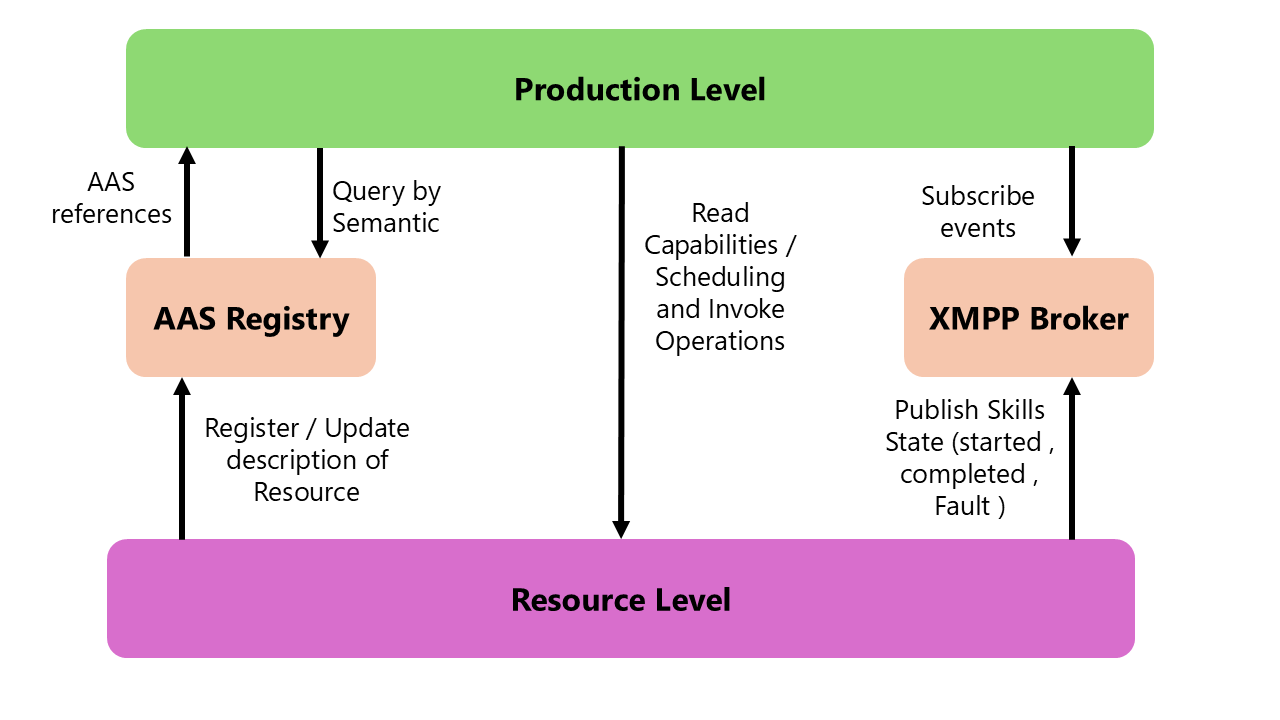
\includegraphics[width=12cm]{Images/system_levels.png}
    \caption{Two-Level System Architecture}
    \label{fig:system_levels}
\end{figure}

\textbf{Product Level.} The product level contains the ProductionAAS, which is responsible for managing production orders and coordinating the allocation of tasks to available resources. When a drilling order is received, the ProductionAAS queries the AAS Registry to discover available resources, retrieves their capabilities, and initiates negotiations to select the most suitable resource for the task. The ProductionAAS subscribes to events published by ResourceAAS instances to monitor execution progress and react to status changes.

\textbf{Resource Level.} The resource level contains one or more ResourceAAS instances, each representing a physical drill machine. ResourceAAS components register themselves with the AAS Registry upon initialization, making their capabilities discoverable. During operation, ResourceAAS instances publish status events (started, completed, fault) to the XMPP Broker, enabling real-time monitoring by the ProductionAAS and other system components. When assigned a production task, the ResourceAAS agent autonomously executes the drilling operation by invoking standardized \ac{AAS} Operations on the physical asset.

\subsection{System Components}
The complete system comprises five main components that work together to realize \ac{Type3AAS} functionality. Figure~\ref{fig:system_architecture} illustrates the overall system architecture and the relationships between components.


\begin{figure}[p]
    \centering
    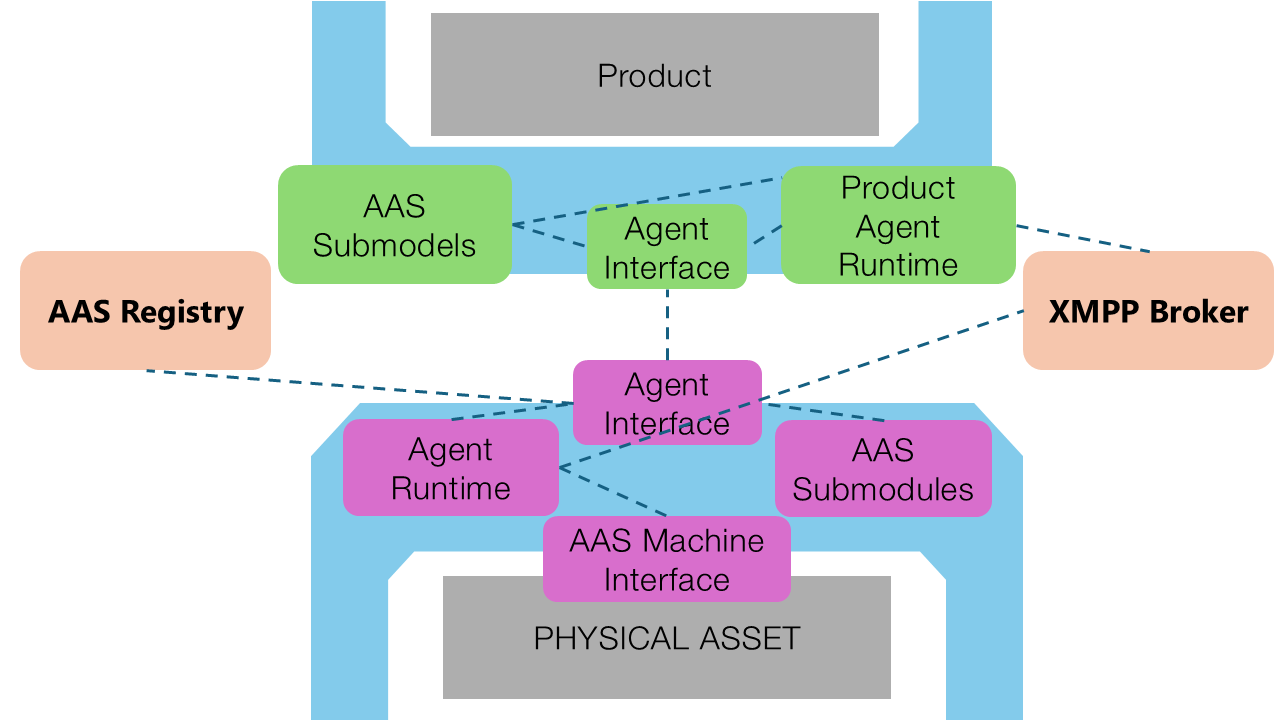
\includegraphics[width=14cm]{Images/system_architecture.png}
    \caption{SmartDrillSystem Architecture Overview}
    \label{fig:system_architecture}
\end{figure}

\textbf{ProductionAAS.} The ProductionAAS serves as the coordination hub for production orders. It combines standardized \ac{AAS} submodels with a \ac{BDI} agent runtime that provides autonomous decision-making capabilities. The ProductionAAS contains submodels for identification, process planning, service cataloging, interface endpoints, and execution tracking. Its agent component implements orchestration logic for task decomposition and negotiation protocols for resource selection. Communication with other components occurs through the Agent Interface, which translates between \ac{AAS} data structures and agent beliefs.

\textbf{ResourceAAS.} Each ResourceAAS represents a digital twin of a physical drill machine, integrating \ac{AAS} standardization with autonomous agent behavior. The ResourceAAS contains submodels describing the asset's operational state, knowledge constraints, capabilities, and interaction parameters. A \ac{BDI} agent runtime provides goal-directed behavior, enabling the resource to autonomously respond to production requests, participate in negotiations, and execute assigned tasks. The AAS Machine Interface connects the digital representation to the physical asset, enabling bidirectional data exchange and operation invocation.

\textbf{AAS Registry.} The AAS Registry provides a centralized discovery service compliant with the \ac{AAS} specification. Upon initialization, each ResourceAAS registers its identification information, endpoint addresses, and capability descriptions with the registry. The ProductionAAS queries the registry to discover available resources that match required capabilities. This decoupled discovery mechanism enables dynamic system reconfiguration without hardcoded dependencies between components.

\textbf{XMPP Broker.} The XMPP Broker implements the event-driven communication infrastructure using the \ac{XMPP} protocol. This choice aligns with the SPADE framework used for agent implementation, which natively supports \ac{XMPP} for agent communication. The broker enables publish-subscribe messaging patterns where ResourceAAS instances publish status events (skill started, completed, or failed) and the ProductionAAS subscribes to receive these updates. This asynchronous communication model supports reactive agent behavior and real-time monitoring.

\textbf{Physical Assets.} The physical drill machines represent the actual manufacturing resources controlled by the system. Each asset connects to its corresponding ResourceAAS through a machine interface that abstracts the underlying communication protocol (such as OPC UA or proprietary interfaces). The ResourceAAS reads sensor data and operational status from the asset and invokes operations to execute drilling tasks.
\subsection{Component Interactions}
Figure~\ref{fig:component_interactions} illustrates the interaction patterns between system components during typical operation.


\begin{figure}[p]
    \centering
    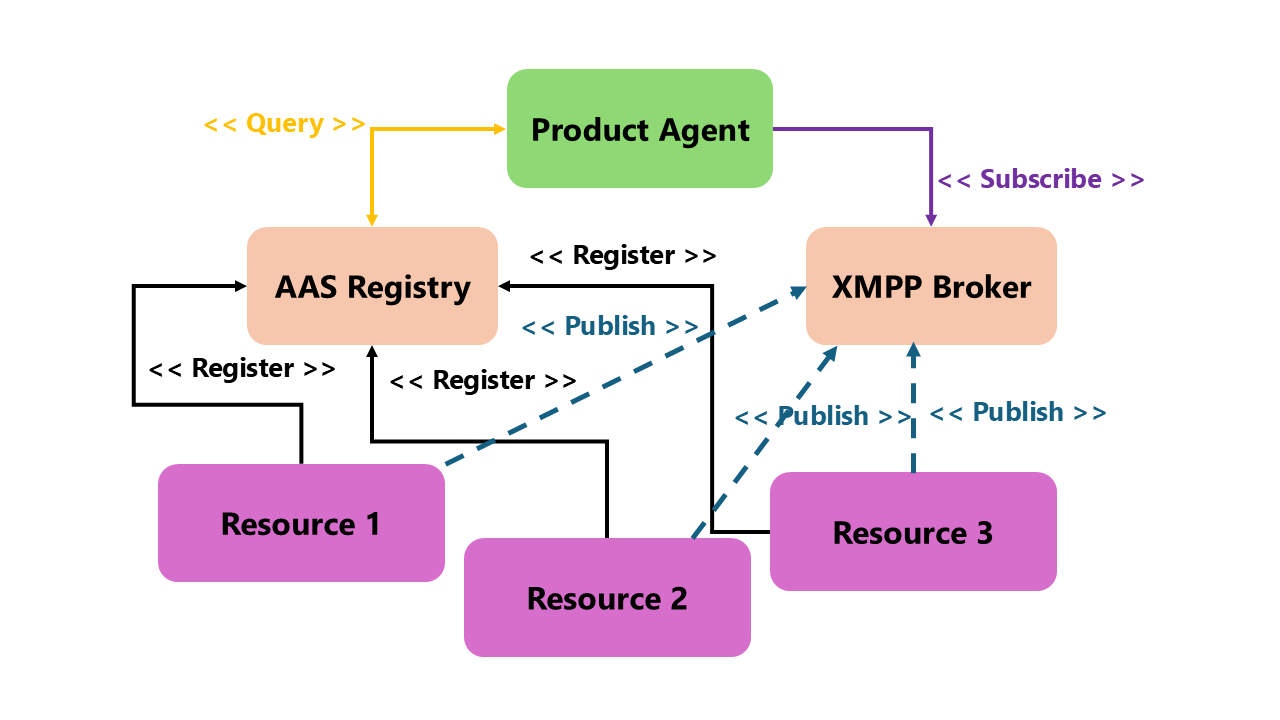
\includegraphics[width=12cm]{Images/component_interactions.png}
    \caption{Component Interaction Patterns}
    \label{fig:component_interactions}
\end{figure}

The system employs four primary interaction patterns:

\textbf{Registration.} During system startup, each ResourceAAS registers itself with the AAS Registry and the XMPP Broker. Registration with the registry enables discovery by the ProductionAAS, while registration with the broker enables event publication and subscription.

\textbf{Discovery.} When the ProductionAAS receives a production order, it queries the AAS Registry to retrieve references to all registered ResourceAAS instances. The registry returns the endpoint addresses and capability descriptions needed to initiate direct communication with resources.

\textbf{Direct Communication.} The ProductionAAS communicates directly with ResourceAAS instances for operations requiring request-response patterns, such as reading capabilities, scheduling information, and invoking operations. This communication uses the standardized \ac{AAS} REST API, ensuring interoperability with the \ac{AAS} specification.

\textbf{Event-Based Communication.} ResourceAAS instances publish status events to the XMPP Broker, and the ProductionAAS subscribes to receive these events. This pattern supports asynchronous notification of state changes without requiring polling, enabling efficient real-time monitoring of distributed resources.


\subsection{Bidirectional AAS Integration}

A key contribution of this design is the bidirectional integration between \ac{BDI} agents and the \ac{AAS} standard. Unlike existing approaches that use \ac{AAS} primarily as a passive data source, this architecture enables agents to both read information from submodels and execute actions through standardized Operations.

\textbf{Beliefs from Submodels.} Agent beliefs are derived from \ac{AAS} submodel data. The Operational State Submodel provides current asset status, the Knowledge Submodel provides constraints and environmental conditions, and the Capability Submodel provides information about available skills. The Agent Interface continuously synchronizes submodel data with the agent's belief base, ensuring that agent decisions reflect the current system state.

\textbf{Intentions through Operations.} Agent intentions are executed through \ac{AAS} Operations defined in the submodels. When an agent commits to executing a drilling task, it invokes the corresponding Operation on the physical asset through the standardized \ac{AAS} API. This approach leverages the Operation element defined in the \ac{AAS} specification, which supports both synchronous and asynchronous invocation patterns.

This bidirectional integration ensures that the autonomous behavior provided by the \ac{BDI} architecture operates within the standardized framework defined by the \ac{AAS} specification, addressing the interoperability requirements identified in Chapter~\ref{ch:literature}.

\subsection{Mapping to RAMI4.0}
\label{subsec:rami40_mapping}

The proposed Type 3 \ac{AAS} architecture can be positioned within the \ac{RAMI4.0} reference model introduced in Chapter~\ref{ch:introduction}. Figure~\ref{fig:RAMI4.0} presents the three-dimensional RAMI4.0 structure consisting of Hierarchy Levels, Life Cycle \& Value Stream, and Layers. This subsection maps the system components to each axis.

\subsubsection{Hierarchy Levels Axis}

The system operates across multiple hierarchy levels as defined by IEC 62264:

\begin{table}[ht]
\centering
\caption{System Components Mapped to RAMI4.0 Hierarchy Levels}
\label{tab:rami_hierarchy}
\begin{tabular}{p{0.20\textwidth}p{0.25\textwidth}p{0.45\textwidth}}
\toprule
\rowcolor{headerblue}
\textcolor{white}{Hierarchy Level} & \textcolor{white}{Component} & \textcolor{white}{Role} \\
\midrule
Work Centers & Production Agent & Coordinates production orders, orchestrates resources \\
\rowcolor{lightgray}
Station & Resource Agent & Manages individual drill machine operations \\
Field Device & Simulators / PLCs & Executes physical operations (drill, move) \\
\bottomrule
\end{tabular}
\end{table}

The Production Agent operates at the \textit{Work Centers} level, receiving production orders and coordinating their execution across available resources. Resource Agents operate at the \textit{Station} level, each representing a single manufacturing resource (drill machine). The simulators (or physical PLCs in a production deployment) represent the \textit{Field Device} level, executing the actual machining operations.

\subsubsection{Life Cycle \& Value Stream Axis}

The RAMI4.0 life cycle axis distinguishes between \textit{Type} (design-time definitions) and \textit{Instance} (runtime representations):

\begin{table}[ht]
\centering
\caption{System Elements Mapped to RAMI4.0 Life Cycle Phases}
\label{tab:rami_lifecycle}
\begin{tabular}{p{0.15\textwidth}p{0.35\textwidth}p{0.40\textwidth}}
\toprule
\rowcolor{headerblue}
\textcolor{white}{Phase} & \textcolor{white}{Type (Design)} & \textcolor{white}{Instance (Runtime)} \\
\midrule
Development & Submodel templates, Capability definitions & -- \\
\rowcolor{lightgray}
Maintenance & Process Plan structure, Knowledge constraints & -- \\
Production & -- & AAS instances, Agent beliefs, Execution state \\
\bottomrule
\end{tabular}
\end{table}

The submodel structures (Capability, Knowledge, Process Plan) represent \textit{Type} information reusable templates that define what a resource can do and how processes are structured. At runtime, these become \textit{Instance} data: concrete AAS instances with actual parameter values, agent beliefs reflecting current state, and execution tracking data that changes during operation.

\subsubsection{Layer Axis}

The six RAMI4.0 layers describe different aspects of an \ac{I4.0} component. Table~\ref{tab:rami_layers} maps the system implementation to each layer:

\begin{table}[ht]
\centering
\caption{System Implementation Mapped to RAMI4.0 Layers}
\label{tab:rami_layers}
\begin{tabular}{p{0.18\textwidth}p{0.72\textwidth}}
\toprule
\rowcolor{headerblue}
\textcolor{white}{Layer} & \textcolor{white}{Implementation} \\
\midrule
Business & Production orders (User Requests) triggering manufacturing processes \\
\rowcolor{lightgray}
Functional & BDI agent logic: goal-directed reasoning, plan execution, CNP negotiation \\
Information & AAS submodels: Capability, Knowledge, Process Plan, Execution Tracking \\
\rowcolor{lightgray}
Communication & XMPP PubSub (agent messaging), REST API (AAS access), HTTP (skill invocation) \\
Integration & ResourceAASClient, invocationDelegation pattern, BaSyx SDK \\
\rowcolor{lightgray}
Asset & Drill machine simulators (proof-of-concept) / Physical PLCs (production) \\
\bottomrule
\end{tabular}
\end{table}

\textbf{Business Layer.} Production orders represent business-level requests that initiate the manufacturing process. The User Request message defines what capability is needed and when.

\textbf{Functional Layer.} The \ac{BDI} agent architecture provides the functional logic. Agents reason about their beliefs (from submodels), form desires (respond to CFP, execute skills), and commit to intentions (negotiate, invoke operations). This layer realizes the ``proactive'' behavior that distinguishes Type 3 from Type 1/2 \ac{AAS}.

\textbf{Information Layer.} The \ac{AAS} submodels provide the standardized information model. All data exchanged between components conforms to the \ac{AAS} meta-model, ensuring interoperability with other I4.0-compliant systems.

\textbf{Communication Layer.} Three protocols handle different communication needs: XMPP PubSub for asynchronous agent messaging and event notification, the \ac{AAS} REST API for submodel access, and HTTP for skill invocation via the invocationDelegation pattern.

\textbf{Integration Layer.} The ResourceAASClient and ProductionAASClient classes bridge the gap between the \ac{AAS} server and the agent runtime. The invocationDelegation qualifier pattern connects \ac{AAS} Operations to external execution endpoints.

\textbf{Asset Layer.} The physical drill machines (represented by simulators in the proof-of-concept) form the asset layer. These execute the actual manufacturing operations when invoked through the integration layer.

\subsubsection{Type 3 AAS in the RAMI4.0 Context}

The key contribution of this work within the RAMI4.0 framework is the enhancement of the \textit{Functional Layer}. While Type 1 and Type 2 \ac{AAS} implementations primarily address the Information, Communication, and Integration layers, the Type 3 \ac{AAS} adds autonomous decision-making capabilities at the Functional Layer through \ac{BDI} agent integration.

This positions the Type 3 \ac{AAS} as an enabler for the RAMI4.0 vision of intelligent, self-organizing production systems where I4.0 components can autonomously coordinate without centralized control.
\section{Resource Agent Concept}
\label{sec:resource_agent}

The ResourceAAS represents the core component for integrating autonomous agent behavior with standardized \ac{AAS} representations of manufacturing resources. This section presents the conceptual design of the ResourceAAS, describing its overall architecture, submodel structure, agent core, and the mechanisms that enable bidirectional integration between the \ac{BDI} agent and the \ac{AAS}.

\subsection{Resource Agent Overview}
\label{subsec:resource_overview}

The ResourceAAS combines three main architectural elements: the \ac{AAS} structure providing standardized data representation, the \ac{BDI} agent core enabling autonomous behavior, and the interfaces connecting these components to each other and to external systems. Figure~\ref{fig:resource_components} illustrates the high-level component structure of the ResourceAAS.

% Include diagram from slide 5
\begin{figure}[p]
    \centering
    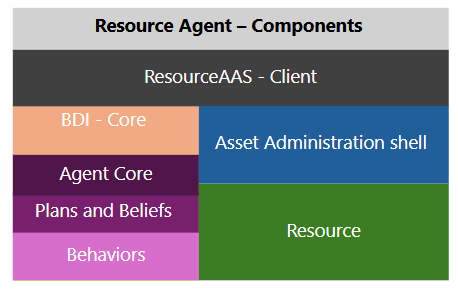
\includegraphics[width=10cm]{Images/resource_components.png}
    \caption{Resource Agent Component Structure}
    \label{fig:resource_components}
\end{figure}

\textbf{Asset Administration Shell.} The \ac{AAS} component provides the standardized digital representation of the drill machine using the Eclipse BaSyx Python SDK. It contains the shell information (identification, asset kind, global asset ID) and a collection of submodels that describe different aspects of the resource. The \ac{AAS} is deployed to a BaSyx AAS Environment server, exposing a REST API that enables external access to submodel data and operation invocation, compliant with the \ac{AAS} API specification defined in Part 2 of the standard.

\textbf{BDI Core.} The \ac{BDI} core implements the agent's autonomous behavior using the SPADE framework combined with the spade\_bdi extension. SPADE (Smart Python Agent Development Environment) provides asynchronous agent communication over \ac{XMPP}, while spade\_bdi adds AgentSpeak-based \ac{BDI} reasoning capabilities. The agent maintains beliefs derived from submodel data, processes desires triggered by external events (such as Call-For-Proposals), and executes intentions through SPADE behaviors. Agent plans are defined in AgentSpeak Language (ASL) files that specify reactive rules for handling events and achieving goals.

\textbf{AAS-Agent Interface (ResourceAASClient).} The ResourceAASClient serves as the translation layer between the \ac{AAS} REST API and the agent's internal representation. This component implements an asynchronous HTTP client using aiohttp that communicates with the BaSyx server via GET and POST requests. It provides repository classes for reading submodel elements (SubmodelElementRepositoryGetters), updating values (SubmodelElementRepositoryUpdate), and invoking operations. The interface translates \ac{AAS} data structures into Python dictionaries that can be converted to agent beliefs.

\textbf{Operation Invokers.} The physical asset operations are exposed through FastAPI-based HTTP endpoints that implement the invocationDelegation pattern specified in the \ac{AAS} Operation qualifiers. When the BaSyx server receives an operation invocation request, it delegates the call to the corresponding invoker endpoint (e.g., \texttt{/drill\_invocation\_1}), which executes the operation on the physical asset or simulator and returns the result.

Figure~\ref{fig:resource_internal} illustrates the internal connections and data flows within the ResourceAAS architecture.

% Include diagram from slide 6 or 16
\begin{figure}[p]
    \centering
    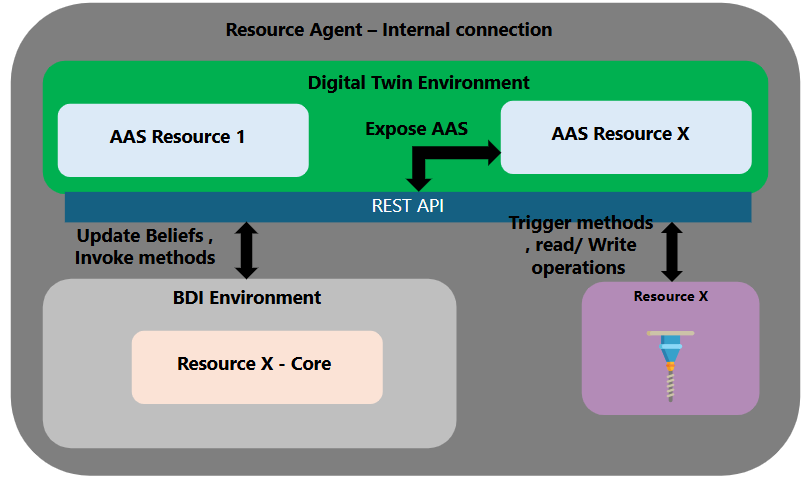
\includegraphics[width=12cm]{Images/resource_internal.png}
    \caption{Resource Agent Internal Architecture}
    \label{fig:resource_internal}
\end{figure}

The architecture supports three primary data flows:

\textbf{Belief Acquisition.} During agent initialization, the AgentInitializationbehavior reads submodel data via the ResourceAASClient and populates the agent's belief base. Beliefs include: \texttt{current\_state} from the Operational State Submodel, \texttt{supported\_skills} from the Capabilities Submodel, \texttt{skills\_constraints} from the Knowledge Submodel, and \texttt{free\_time\_slots} / \texttt{booked\_time\_slots} from the Operational State time slot collection.

\textbf{Event Processing.} When the agent receives a Call-For-Proposal (CFP) from the ProductionAAS via \ac{XMPP} publish-subscribe, the CFPProcessingbehavior validates the request against current beliefs. It checks whether the resource state allows execution, whether the requested skill is supported, and whether input parameters fall within the constraints defined in the Knowledge Submodel.

\textbf{Operation Execution.} When the agent commits to executing a task, the corresponding invoker behavior (e.g., DrillInvokerbehavior) retrieves input parameters from beliefs, calls the operation through the ResourceAASClient, and updates beliefs with the result. The operation invocation follows the \ac{AAS} standard, passing through the BaSyx server to the delegated FastAPI endpoint.

\subsection{Resource Agent Submodels}
\label{subsec:resource_submodels}

The ResourceAAS contains four submodels that provide the standardized data structures supporting agent operation. These submodels are implemented using the Eclipse BaSyx Python SDK and are designed to map directly to the \ac{BDI} components. The following subsections describe each submodel based on the actual implementation.


\subsubsection{Operational State Submodel}

The Operational State Submodel captures the current runtime status and scheduling information of the resource. It provides the primary source for agent beliefs about the asset's availability and current condition. Figure~\ref{fig:sm_operational_state} shows the structure of this submodel.

\begin{figure}[p]
    \centering
    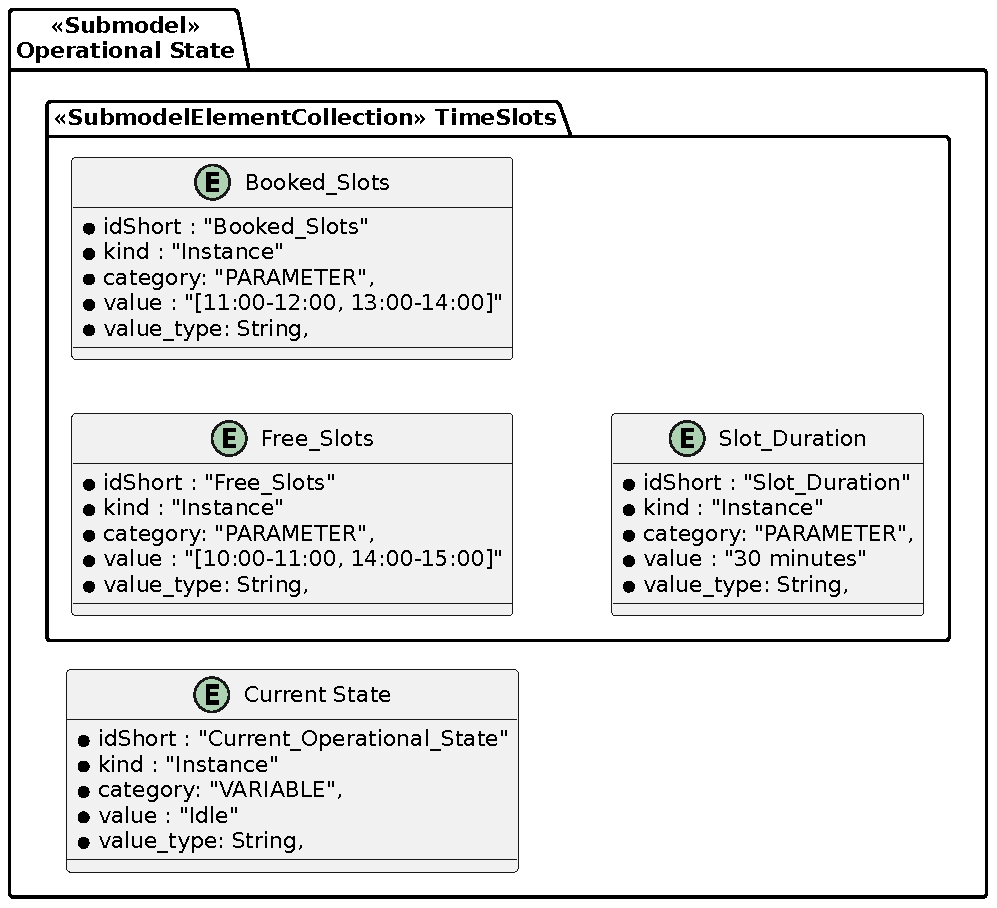
\includegraphics[width=0.85\textwidth]{Images/sm_operational_state.pdf}
    \caption{Operational State Submodel Structure}
    \label{fig:sm_operational_state}
\end{figure}

\textbf{Current\_Operational\_State.} This Property element tracks the real-time operational status of the drill machine. The value contains the current state as a string (``Idle'', ``Running'', ``Error'', or ``Done''), with the category set to ``VARIABLE'' indicating runtime mutability. During CFP processing, the agent checks this belief to ensure the resource is in an allowed state (``Idle'' or ``Free'') before accepting new tasks.

\textbf{TimeSlots\_Operational\_Data.} This SubmodelElementCollection manages the resource's scheduling information through three properties:
\begin{itemize}
    \item \texttt{Free\_Slots}: JSON-encoded list of available time slots (e.g., ``08:00'', ``08:30'', ``09:00'')
    \item \texttt{Booked\_Slots}: JSON-encoded list of already allocated time slots
    \item \texttt{Slot\_Duration}: Integer value representing the duration of each slot in minutes
\end{itemize}
The TimeSlotDataType class manages slot allocation and release, ensuring that negotiation decisions are based on actual availability.

\subsubsection{Knowledge Submodel}

The Knowledge Submodel contains constraint information that defines the operational boundaries of the resource. This information is used during CFP validation to determine whether requested parameters are feasible. Figure~\ref{fig:sm_knowledge} shows the structure of this submodel.
\subsubsection{Knowledge Submodel}

The Knowledge Submodel contains constraint information that defines the operational boundaries of the resource. This information is used during CFP validation to determine whether requested parameters are feasible. Figure~\ref{fig:sm_knowledge} shows the structure of this submodel.

\begin{figure}[p]
    \centering
    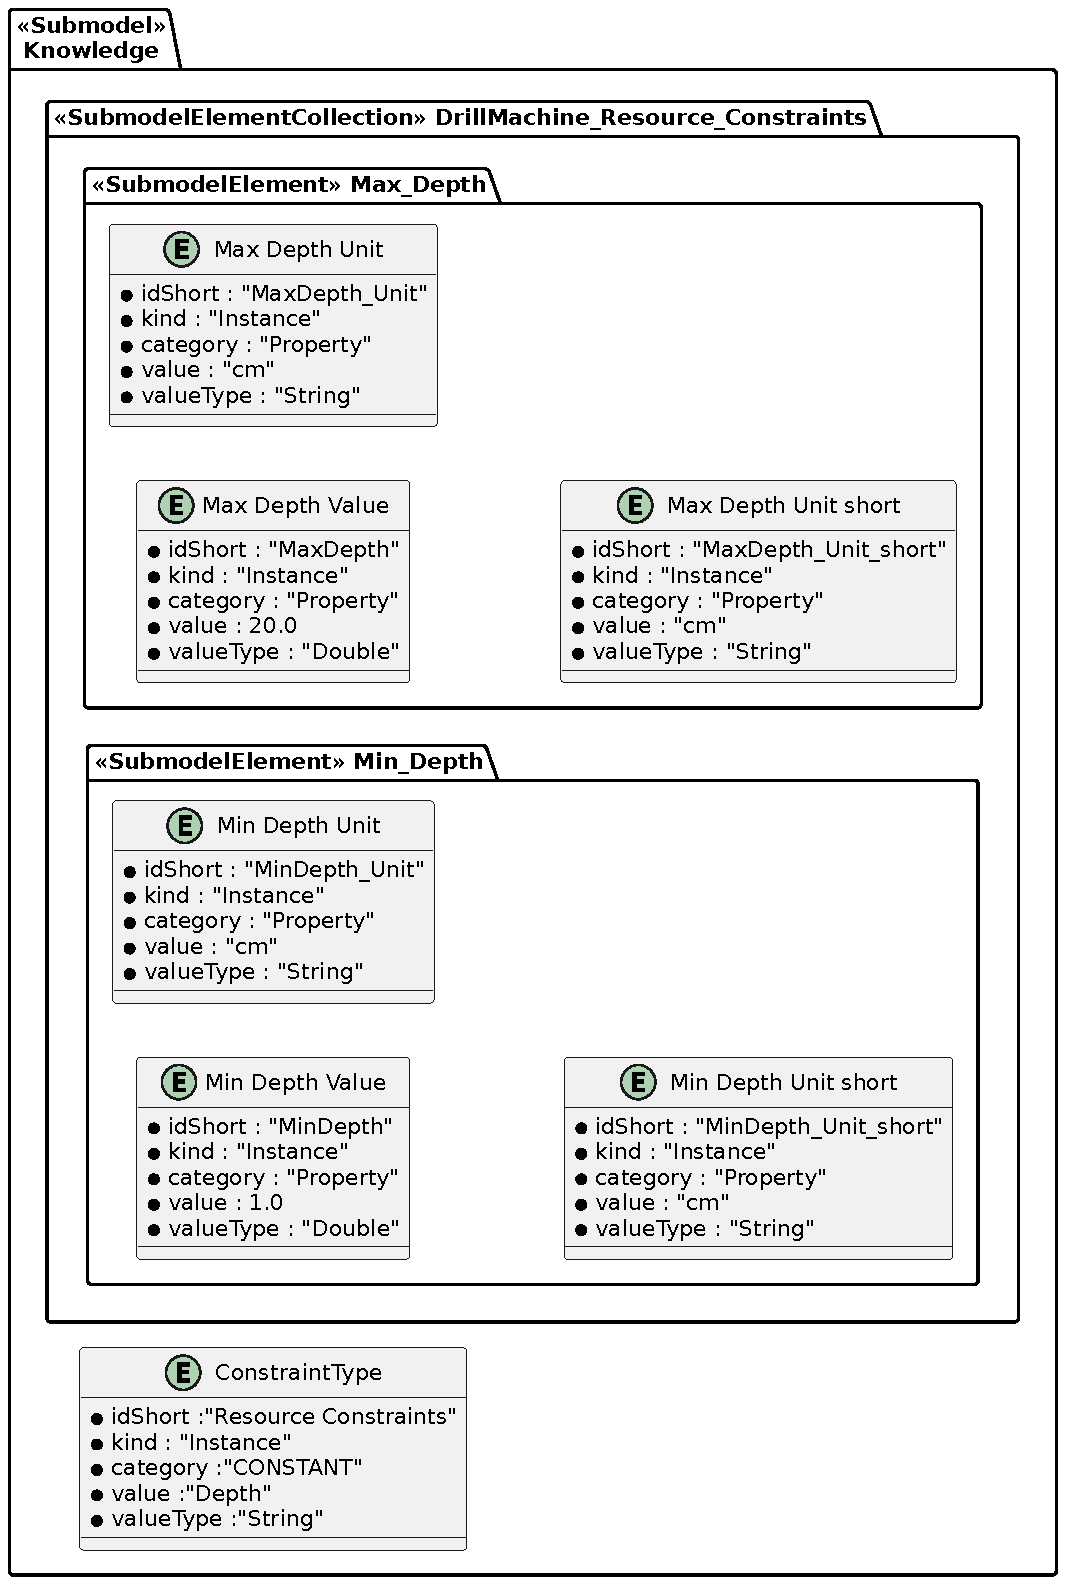
\includegraphics[width=0.85\textwidth]{Images/sm_knowledge.pdf}
    \caption{Knowledge Submodel Structure}
    \label{fig:sm_knowledge}
\end{figure}

\textbf{Resource\_Constraints.} This SubmodelElementCollection contains nested collections for each constraint type:
\begin{itemize}
    \item \texttt{MaxDepth}: Collection with MaxDepthValue (Double, e.g., 20.0), MaxDepthUnit (``centimeters''), and MaxDepthUnitShort (``cm'')
    \item \texttt{MinDepth}: Collection with MinDepthValue (Double, e.g., 1.0) and corresponding unit properties
    \item \texttt{ConstraintType}: Property indicating the parameter being constrained (``Depth'')
\end{itemize}

During CFP processing, the agent retrieves the constraint type and min/max values, then validates that the requested input parameter falls within the allowed range. If validation fails, a \texttt{CONSTRAINT\_VIOLATION} is added to the negotiation response.

\subsubsection{Capability Submodel}

The Capability Submodel describes the skills and operations that the resource can perform. This submodel directly relates to agent capabilities and contains the Operation elements that enable bidirectional integration. Figure~\ref{fig:sm_capability} shows the structure of this submodel.

\begin{figure}[p]
    \centering
    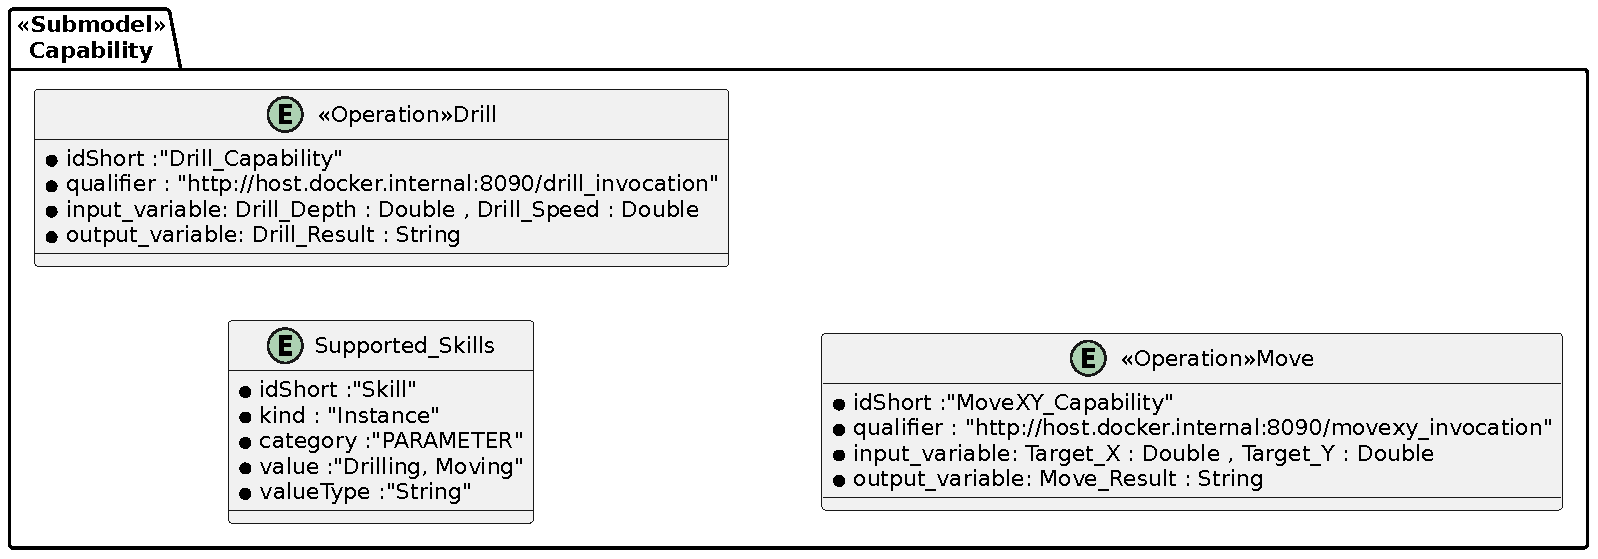
\includegraphics[width=0.95\textwidth]{Images/sm_capability.pdf}
    \caption{Capability Submodel Structure}
    \label{fig:sm_capability}
\end{figure}

\textbf{Supported\_Skills.} This Property lists the capabilities supported by the resource as a comma-separated string (e.g., ``drill\_capability,movexy\_capability''). The ProductionAAS uses this information during resource discovery to filter resources that can fulfill requested operations.

\textbf{Drill\_Capability.} This Operation element defines the drilling capability with:
\begin{itemize}
    \item \texttt{invocationDelegation} qualifier: URL of the FastAPI endpoint
    \item Input variables: Drill\_Depth (Double) and Drill\_Speed (Double)
    \item Output variable: Drill\_Result (String)
\end{itemize}

\textbf{MoveXY\_Capability.} This Operation element defines the positioning capability with:
\begin{itemize}
    \item \texttt{invocationDelegation} qualifier: URL of the movement endpoint
    \item Input variables: Target\_X (Double) and Target\_Y (Double)
    \item Output variable: Move\_Result (String)
\end{itemize}

The invocationDelegation pattern enables the BaSyx server to forward operation requests to external services, supporting integration with physical assets or simulators without modifying the \ac{AAS} infrastructure.

\subsubsection{Interaction and Scheduling Submodel}

The Interaction and Scheduling Submodel provides the communication endpoints through which external systems can interact with the ResourceAAS. Figure~\ref{fig:sm_interaction} shows the structure of this submodel.

\begin{figure}[p]
    \centering
    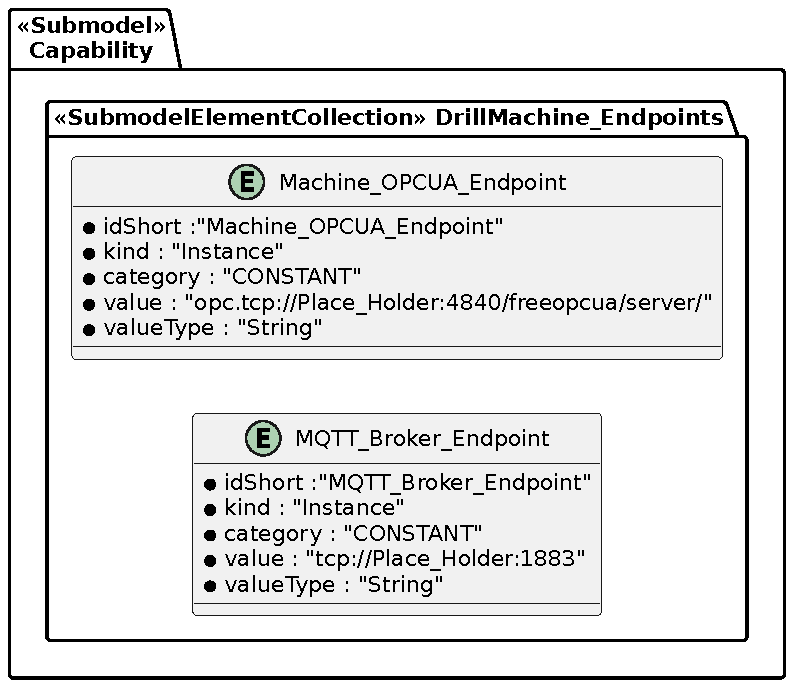
\includegraphics[width=0.6\textwidth]{Images/sm_interaction.pdf}
    \caption{Interaction and Scheduling Submodel Structure}
    \label{fig:sm_interaction}
\end{figure}

\textbf{Endpoints.} This SubmodelElementCollection contains properties for different communication protocols:
\begin{itemize}
    \item \texttt{Machine\_OPCUA\_Endpoint}: OPC UA server address for direct asset communication (placeholder for future integration)
    \item \texttt{MQTT\_Broker\_Endpoint}: MQTT broker address for event-based communication
\end{itemize}

The ProductionAAS retrieves these endpoints during the discovery phase to establish appropriate communication channels for negotiation and task assignment.


\subsection{BDI-Submodel Integration}
\label{sec:bdi_submodel_integration}

This section explicitly describes how the \ac{BDI} architecture manifests in the Type 3 \ac{AAS} implementation. The title of this thesis references \ac{BDI} agents, and this section clarifies how Beliefs, Desires, and Intentions are concretely realized through the \ac{AAS} submodels and AgentSpeak plans.
\subsubsection{Conceptual Mapping}

The \ac{BDI} model defines three mental attitudes that govern agent behavior:
\begin{itemize}
    \item \textbf{Beliefs}: The agent's knowledge about itself, other agents, and the environment
    \item \textbf{Desires}: The agent's objectives or goals it wishes to achieve
    \item \textbf{Intentions}: The agent's committed plans for achieving its goals
\end{itemize}
In the Type 3 \ac{AAS} architecture, these mental attitudes are distributed between the \ac{AAS} submodels (persistent, shared state) and the AgentSpeak plans (reactive behavior). Table~\ref{tab:bdi_mapping} provides the concrete mapping.

\begin{table}[p]
\centering
\caption{BDI to AAS-Agent Mapping}
\label{tab:bdi_mapping}
\begin{tabular}{p{0.12\textwidth}p{0.28\textwidth}p{0.48\textwidth}}
\toprule
\rowcolor{headerblue}
\textcolor{white}{BDI Element} & \textcolor{white}{AAS/Agent Component} & \textcolor{white}{Concrete Example} \\
\midrule
Beliefs & Operational State Submodel & \texttt{current\_state}, \texttt{free\_time\_slots} \\
        & Knowledge Submodel & \texttt{skills\_constraints}, \texttt{skills\_constraints\_types} \\
        & Capability Submodel & \texttt{supported\_skills} \\
        & Runtime Beliefs & \texttt{is\_cfp\_received}, \texttt{cfp\_skill}, \texttt{cfp\_at\_time} \\
\midrule
\rowcolor{lightgray}
Desires & AgentSpeak Goals & \texttt{!setup} (initialization goal) \\
\rowcolor{lightgray}
        & Event-triggered Goals & Respond to CFP, execute skills \\
\rowcolor{lightgray}
        & Process Plan & Reach \texttt{Exit\_Point} from \texttt{Entry\_Point} \\
\midrule
Intentions & AgentSpeak Plans & Plans triggered by belief additions \\
           & Custom Actions & \texttt{.initialize\_agent}, \texttt{.process\_cfp}, \texttt{.drill} \\
           & SPADE behaviors & \texttt{DrillInvokerbehavior}, \texttt{MoveXYInvokerbehavior} \\
\bottomrule
\end{tabular}
\end{table}

\subsubsection{Beliefs: AAS Submodels as Knowledge Base}

The agent's beliefs are loaded from \ac{AAS} submodels during initialization via the \texttt{AgentInitializationbehavior}. This behavior reads submodel data and converts it to agent beliefs:

\begin{lstlisting}[language=Python, caption={Belief Loading from AAS Submodels}, label={lst:belief_loading}]
class AgentInitializationbehavior(OneShotbehavior):
    async def run(self):
        # Load beliefs from AAS submodels concurrently
        current_state, skills, constraints, ... = await asyncio.gather(
            self.agent.resource_client.getvalue_Current_State(),
            self.agent.resource_client.getvalue_Supported_Skills(),
            self.agent.resource_client.getvalue_MaxMinDepth(),
            self.agent.resource_client.getvalue_Free_Slots(),
            ...
        )
        # Set beliefs in BDI agent
        self.agent.bdi.set_belief("current_state", current_state)
        self.agent.bdi.set_belief("supported_skills", skills)
        self.agent.bdi.set_belief("skills_constraints", constraints)
        self.agent.bdi.set_belief("free_time_slots", free_time_slots)
\end{lstlisting}
Table~\ref{tab:belief_sources} shows the mapping between \ac{AAS} submodel elements and agent beliefs:

\begin{table}[p]
\centering
\caption{AAS Submodel Elements to Agent Beliefs}
\label{tab:belief_sources}
\begin{tabular}{lll}
\toprule
\rowcolor{headerblue}
\textcolor{white}{Submodel} & \textcolor{white}{Element} & \textcolor{white}{Belief Predicate} \\
\midrule
Operational State & Current\_State & \texttt{current\_state(State)} \\
Operational State & Free\_Slots & \texttt{free\_time\_slots(Slots)} \\
Operational State & Booked\_Slots & \texttt{booked\_time\_slots(Slots)} \\
\rowcolor{lightgray}
Capability & Supported\_Skills & \texttt{supported\_skills(Skills)} \\
\rowcolor{lightgray}
Knowledge & Constraints & \texttt{skills\_constraints(Values)} \\
Knowledge & Constraints\_Type & \texttt{skills\_constraints\_types(Types)} \\
\bottomrule
\end{tabular}
\end{table}
\textbf{Runtime Beliefs.} In addition to persistent beliefs from submodels, the agent maintains runtime beliefs that change during execution:
\begin{itemize}
    \item \texttt{is\_cfp\_received(true/false)}: Set when a CFP message arrives
    \item \texttt{cfp\_skill(Skill)}: The requested capability from the CFP
    \item \texttt{cfp\_at\_time(TimeSlot)}: The requested time slot
    \item \texttt{current\_operation(drill/movexy)}: Tracks which operation is executing
    \item \texttt{drill\_completed(true)}, \texttt{move\_xy\_completed(true)}: Operation completion flags
\end{itemize}

\subsubsection{Desires: Goals in AgentSpeak}

Desires represent what the agent wants to achieve. In the implementation, desires are expressed through AgentSpeak achievement goals and event-triggered responses:

\textbf{Initialization Goal.} The agent starts with an explicit goal:
\begin{lstlisting}[language=Prolog, caption={Initial Goal in AgentSpeak}, label={lst:initial_goal}]
!setup.

+!setup <-
  .print("Agent started : Drilling Machine 1");
  .initialize_agent;
  .check_request.
\end{lstlisting}

\textbf{Event-Triggered Desires.} Most desires emerge from belief changes rather than explicit goal statements. When a belief is added, it triggers a plan that implicitly represents a desire:

\begin{lstlisting}[language=Prolog, caption={Desire: Respond to CFP}, label={lst:cfp_desire}]
// Desire: When CFP received, respond appropriately
+is_cfp_received(true) <-
  -is_cfp_received(true);
  .print("EVENT: CFP received, processing Time slots");
  .process_time_slots;
  .process_cfp.
\end{lstlisting}

\begin{lstlisting}[language=Prolog, caption={Desire: Execute Skills}, label={lst:execute_desire}]
// Desire: When selected, execute the requested skills
+excute_skills(drill_capability) <-
  -excute_skills(drill_capability);
  +current_operation(drill);
  .print("Drilling - starting move_xy");
  .move_xy.
\end{lstlisting}

\subsubsection{Intentions: Committed Plans and Actions}
Intentions are the plans the agent commits to execute. They bridge desires to concrete actions through custom actions and SPADE behaviors:

\textbf{Custom Actions.} The \texttt{ResourceAgent} class registers custom actions that map AgentSpeak action calls to SPADE behaviors:

\begin{lstlisting}[language=Python, caption={Custom Action Registration}, label={lst:custom_actions}]
def add_custom_actions(self, actions):
    @actions.add(".initialize_agent", 0)
    def _initialize_agent(agent, term, intention):
        agent_init_behavior = AgentInitializationbehavior()              
        self.add_behavior(agent_init_behavior)
        yield
        
    @actions.add(".drill", 0)
    def _drill(agent, term, intention):
        drill_behavior = DrillInvokerbehavior()
        self.add_behavior(drill_behavior)
        yield
        
    @actions.add(".move_xy", 0)
    def _move_xy(agent, term, intention):
        move_xy_behavior = MoveXYInvokerbehavior()
        self.add_behavior(move_xy_behavior)
        yield
\end{lstlisting}

\textbf{Intention Execution Flow.} When an AgentSpeak plan executes an action like \texttt{.drill}, the following occurs:
\begin{enumerate}
    \item AgentSpeak interpreter calls the registered custom action
    \item Custom action instantiates the corresponding SPADE behavior
    \item behavior executes asynchronously, invoking the \ac{AAS} Operation
    \item Upon completion, behavior sets a belief (e.g., \texttt{drill\_completed(true)})
    \item Belief change triggers the next plan in the sequence
\end{enumerate}

\textbf{Context-Dependent Plans.} AgentSpeak supports context conditions that select different plans based on current beliefs:

\begin{lstlisting}[language=Prolog, caption={Context-Dependent Intention Selection}, label={lst:context_plans}]
// When move completes during drill operation -> continue to drill
+move_xy_completed(true) : current_operation(drill) <-
  -move_xy_completed(true);
  .print("Move completed, now drilling");
  .drill.

// When move completes during movexy-only operation -> done
+move_xy_completed(true) : current_operation(movexy) <-
  -move_xy_completed(true);
  -current_operation(movexy);
  .print("Move completed, operation done");
  .operation_done.
\end{lstlisting}

This demonstrates how the agent's current beliefs (context) determine which intention is formed, a key characteristic of \ac{BDI} reasoning.
\subsubsection{BDI Reasoning Cycle}
Figure~\ref{fig:bdi_cycle} illustrates how the \ac{BDI} reasoning cycle operates within the Type 3 \ac{AAS}:

\begin{figure}[ht]
\centering
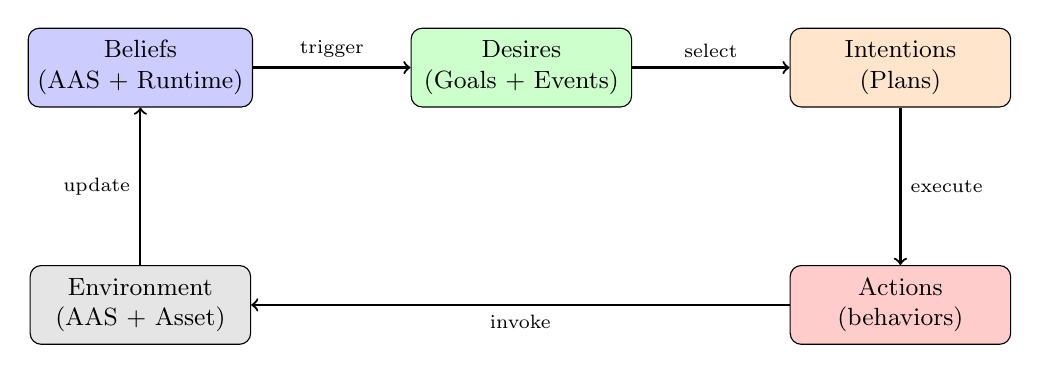
\begin{tikzpicture}[node distance=2cm, auto,
    box/.style={rectangle, draw, rounded corners, minimum width=2.8cm, minimum height=1cm, align=center, font=\small},
    arrow/.style={->, thick}]
    
    \node[box, fill=blue!20] (beliefs) {Beliefs\\(AAS + Runtime)};
    \node[box, fill=green!20, right=of beliefs] (desires) {Desires\\(Goals + Events)};
    \node[box, fill=orange!20, right=of desires] (intentions) {Intentions\\(Plans)};
    \node[box, fill=red!20, below=of intentions] (actions) {Actions\\(behaviors)};
    \node[box, fill=gray!20, below=of beliefs] (environment) {Environment\\(AAS + Asset)};
    
    \draw[arrow] (beliefs) -- (desires) node[midway, above, font=\scriptsize] {trigger};
    \draw[arrow] (desires) -- (intentions) node[midway, above, font=\scriptsize] {select};
    \draw[arrow] (intentions) -- (actions) node[midway, right, font=\scriptsize] {execute};
    \draw[arrow] (actions) -- (environment) node[midway, below, font=\scriptsize] {invoke};
    \draw[arrow] (environment) -- (beliefs) node[midway, left, font=\scriptsize] {update};
    
\end{tikzpicture}
\caption{BDI Reasoning Cycle in Type 3 AAS}
\label{fig:bdi_cycle}
\end{figure}

\begin{enumerate}
    \item \textbf{Beliefs}: Agent loads beliefs from \ac{AAS} submodels and receives runtime belief updates
    \item \textbf{Trigger}: Belief additions trigger AgentSpeak plan selection
    \item \textbf{Select}: Agent selects applicable plan based on context conditions
    \item \textbf{Execute}: Plan body executes, calling custom actions
    \item \textbf{Invoke}: Custom actions invoke SPADE behaviors that call \ac{AAS} Operations
    \item \textbf{Update}: Operation results update beliefs, continuing the cycle
\end{enumerate}

\subsubsection{Example: Complete CFP Response Cycle}
To illustrate the \ac{BDI} cycle, consider how a Resource Agent responds to a Call-For-Proposal:
\begin{enumerate}
    \item \textbf{Belief}: \texttt{ProductionRequestbehavior} receives CFP message, sets \texttt{is\_cfp\_received(true)}
    
    \item \textbf{Plan Triggered}: AgentSpeak matches plan for \texttt{+is\_cfp\_received(true)}
    
    \item \textbf{Intention}: Agent commits to plan body:
    \begin{lstlisting}[language=Prolog, numbers=none]
.process_time_slots;
.process_cfp.
    \end{lstlisting}
    
    \item \textbf{Action}: \texttt{.process\_time\_slots} $\rightarrow$ \texttt{TimeSlotProcessingbehavior}
    \begin{itemize}
        \item Checks \texttt{free\_time\_slots} belief against requested time
        \item Sets \texttt{is\_negotiation\_message\_ready(true)}
    \end{itemize}
    
    \item \textbf{Next Plan}: \texttt{+is\_negotiation\_message\_ready(true)} triggers response plan
    
    \item \textbf{Action}: \texttt{.inform\_production\_agent} $\rightarrow$ \texttt{InformProductionAgent}
    \begin{itemize}
        \item Publishes proposal to XMPP topic
    \end{itemize}
    
    \item \textbf{Belief Update}: Production Agent's decision arrives, setting either:
    \begin{itemize}
        \item \texttt{is\_negotiation\_response\_positive(true)} $\rightarrow$ prepare execution
        \item \texttt{is\_negotiation\_response\_positive(false)} $\rightarrow$ return to waiting
    \end{itemize}
\end{enumerate}
This cycle demonstrates how \ac{BDI} mental attitudes beliefs from \ac{AAS} submodels, desires expressed as reactive plans, and intentions executed through behaviors combine to produce autonomous, goal-directed behavior in the Type 3 \ac{AAS}.
%%%%%%%%%%%%%%%%%%%% 

\newpage
\subsection{Resource Agent Repositories}
\label{subsec:resource_repositories}

The communication between the \ac{BDI} agent and the \ac{AAS} server requires a structured data access layer that abstracts the complexity of REST API interactions. The Repository design pattern~\cite{fowler2002patterns} provides this abstraction, enabling clean separation between agent logic and \ac{AAS} communication. Figure~\ref{fig:repository_architecture} illustrates the repository class hierarchy.

\begin{landscape}
    

\begin{figure}[p]
    \centering
    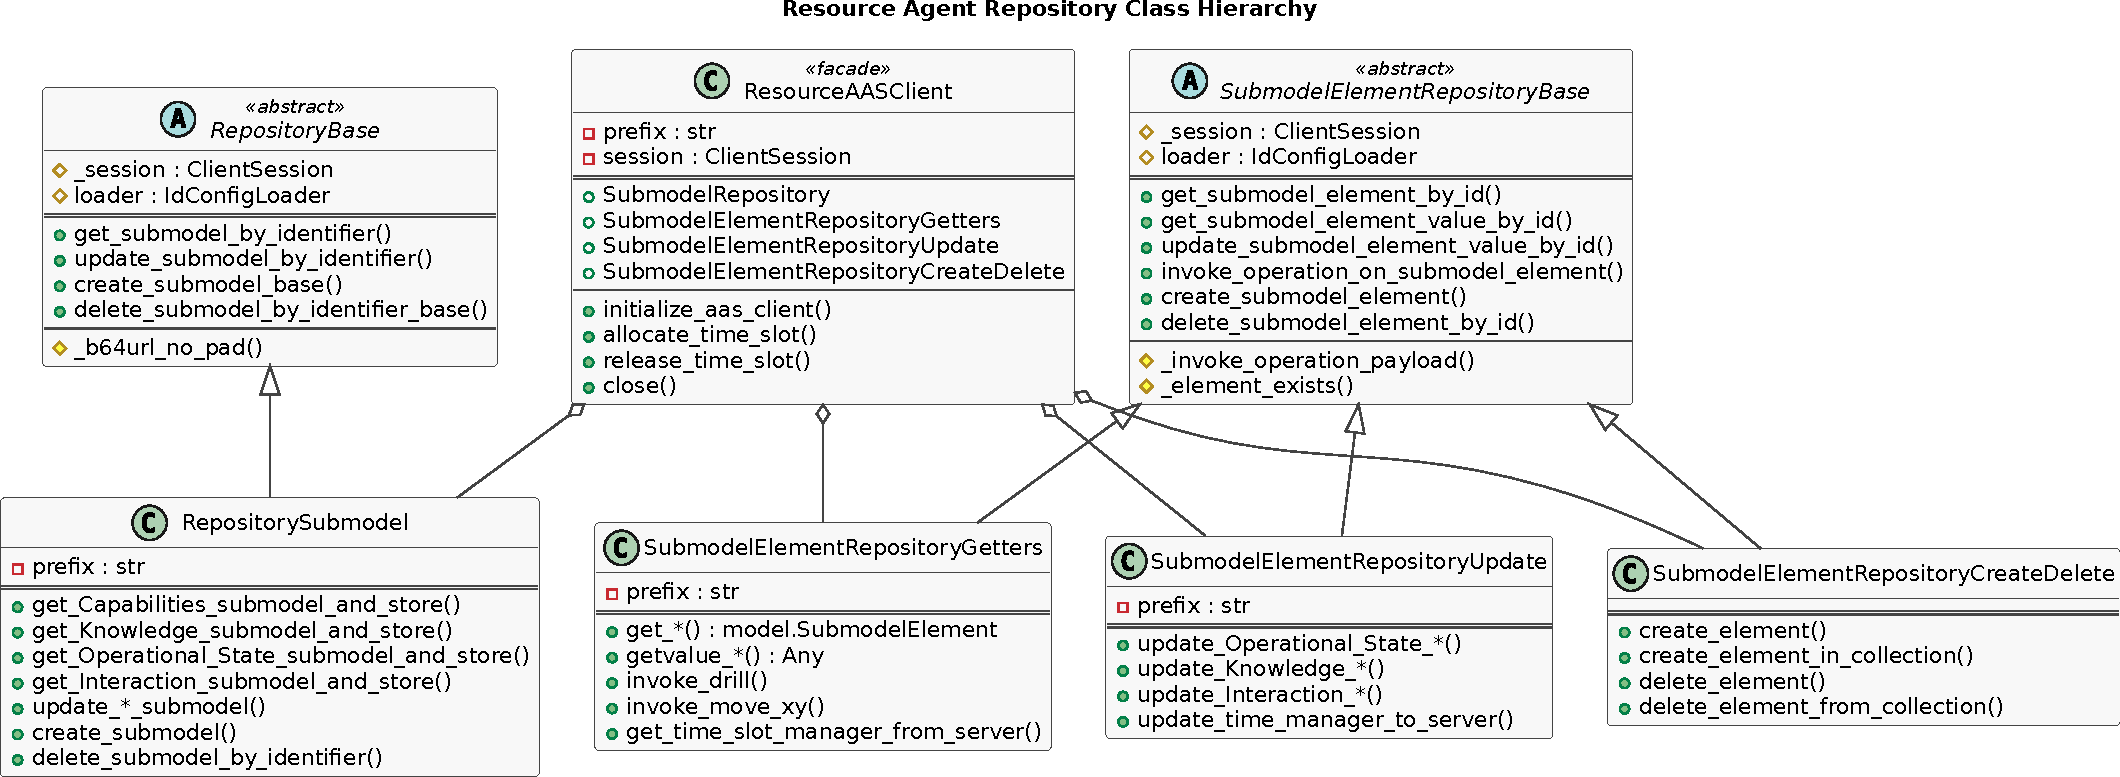
\includegraphics[width=24cm]{Images/repository_hierarchy.pdf}
    \caption{Resource Agent Repository Class Hierarchy}
    \label{fig:repository_architecture}
\end{figure}
\end{landscape}
\subsubsection{Base Classes}

\textbf{RepositoryBase} serves as the abstract foundation for Submodel-level operations. It encapsulates HTTP session management using aiohttp, Base64 URL-safe encoding for \ac{AAS} identifiers (as required by the BaSyx API), and JSON serialization using BaSyx SDK encoders. This class provides generic CRUD operations for retrieving, updating, creating, and deleting entire Submodels.

\textbf{SubmodelElementRepositoryBase} extends the base functionality for SubmodelElement-level operations. It handles path-based element access using dot notation for nested collections (e.g., \texttt{Collection.Property}), operation invocation with automatic payload construction, and idempotent element creation with existence checks.


\subsubsection{Specialized Repositories}

\textbf{RepositorySubmodel} inherits from RepositoryBase and provides Submodel-specific methods for each of the four ResourceAAS submodels. It includes a prefix injection mechanism that enables support for multiple resource instances (e.g., Drill\_1, Drill\_2) by dynamically modifying submodel identifiers.

\textbf{SubmodelElementRepositoryGetters} provides read-only access to submodel elements. It follows a dual naming convention: \texttt{get\_*()} methods return complete BaSyx model objects, while \texttt{getvalue\_*()} methods return only the element values. This class also provides operation invocation methods (\texttt{invoke\_drill()}, \texttt{invoke\_move\_xy()}) and utility methods like \texttt{get\_time\_slot\_manager\_from\_server()} for complex data retrieval.

\textbf{SubmodelElementRepositoryUpdate} provides write operations for modifying submodel element values. It mirrors the getter structure with update methods for each element type across all submodels.

\textbf{SubmodelElementRepositoryCreateDelete} handles element lifecycle management, supporting dynamic addition and removal of submodel elements during runtime.

\textbf{ResourceAASClient} acts as a facade that aggregates all repository instances. It is initialized with a resource prefix and provides a single entry point for agent behaviors to access \ac{AAS} data:

\begin{verbatim}
class ResourceAASClient:
    def __init__(self, prefix: str = ""):
        self.prefix = prefix
        
    async def initialize_aas_client(self):
        self.session = aiohttp.ClientSession()
        self.SubmodelRepository = RepositorySubmodel(self.session, self.prefix)
        self.SubmodelElementRepositoryGetters = SubmodelElementRepositoryGetters(
            self.session, self.prefix)
        self.SubmodelElementRepositoryUpdate = SubmodelElementRepositoryUpdate(
            self.session, self.prefix)
\end{verbatim}

This layered architecture ensures that the agent core remains decoupled from REST API details, facilitating testing and maintenance.

\subsection{Resource Agent Core}
\label{subsec:resource_agent_core}

The Resource Agent Core implements the \ac{BDI} reasoning cycle that enables autonomous behavior. This subsection describes the agent class structure, the AgentSpeak plans, and the SPADE behaviors that execute agent actions. Figure~\ref{fig:resource_agent_core} illustrates the class architecture.

    

\begin{figure}[p]
    \centering
    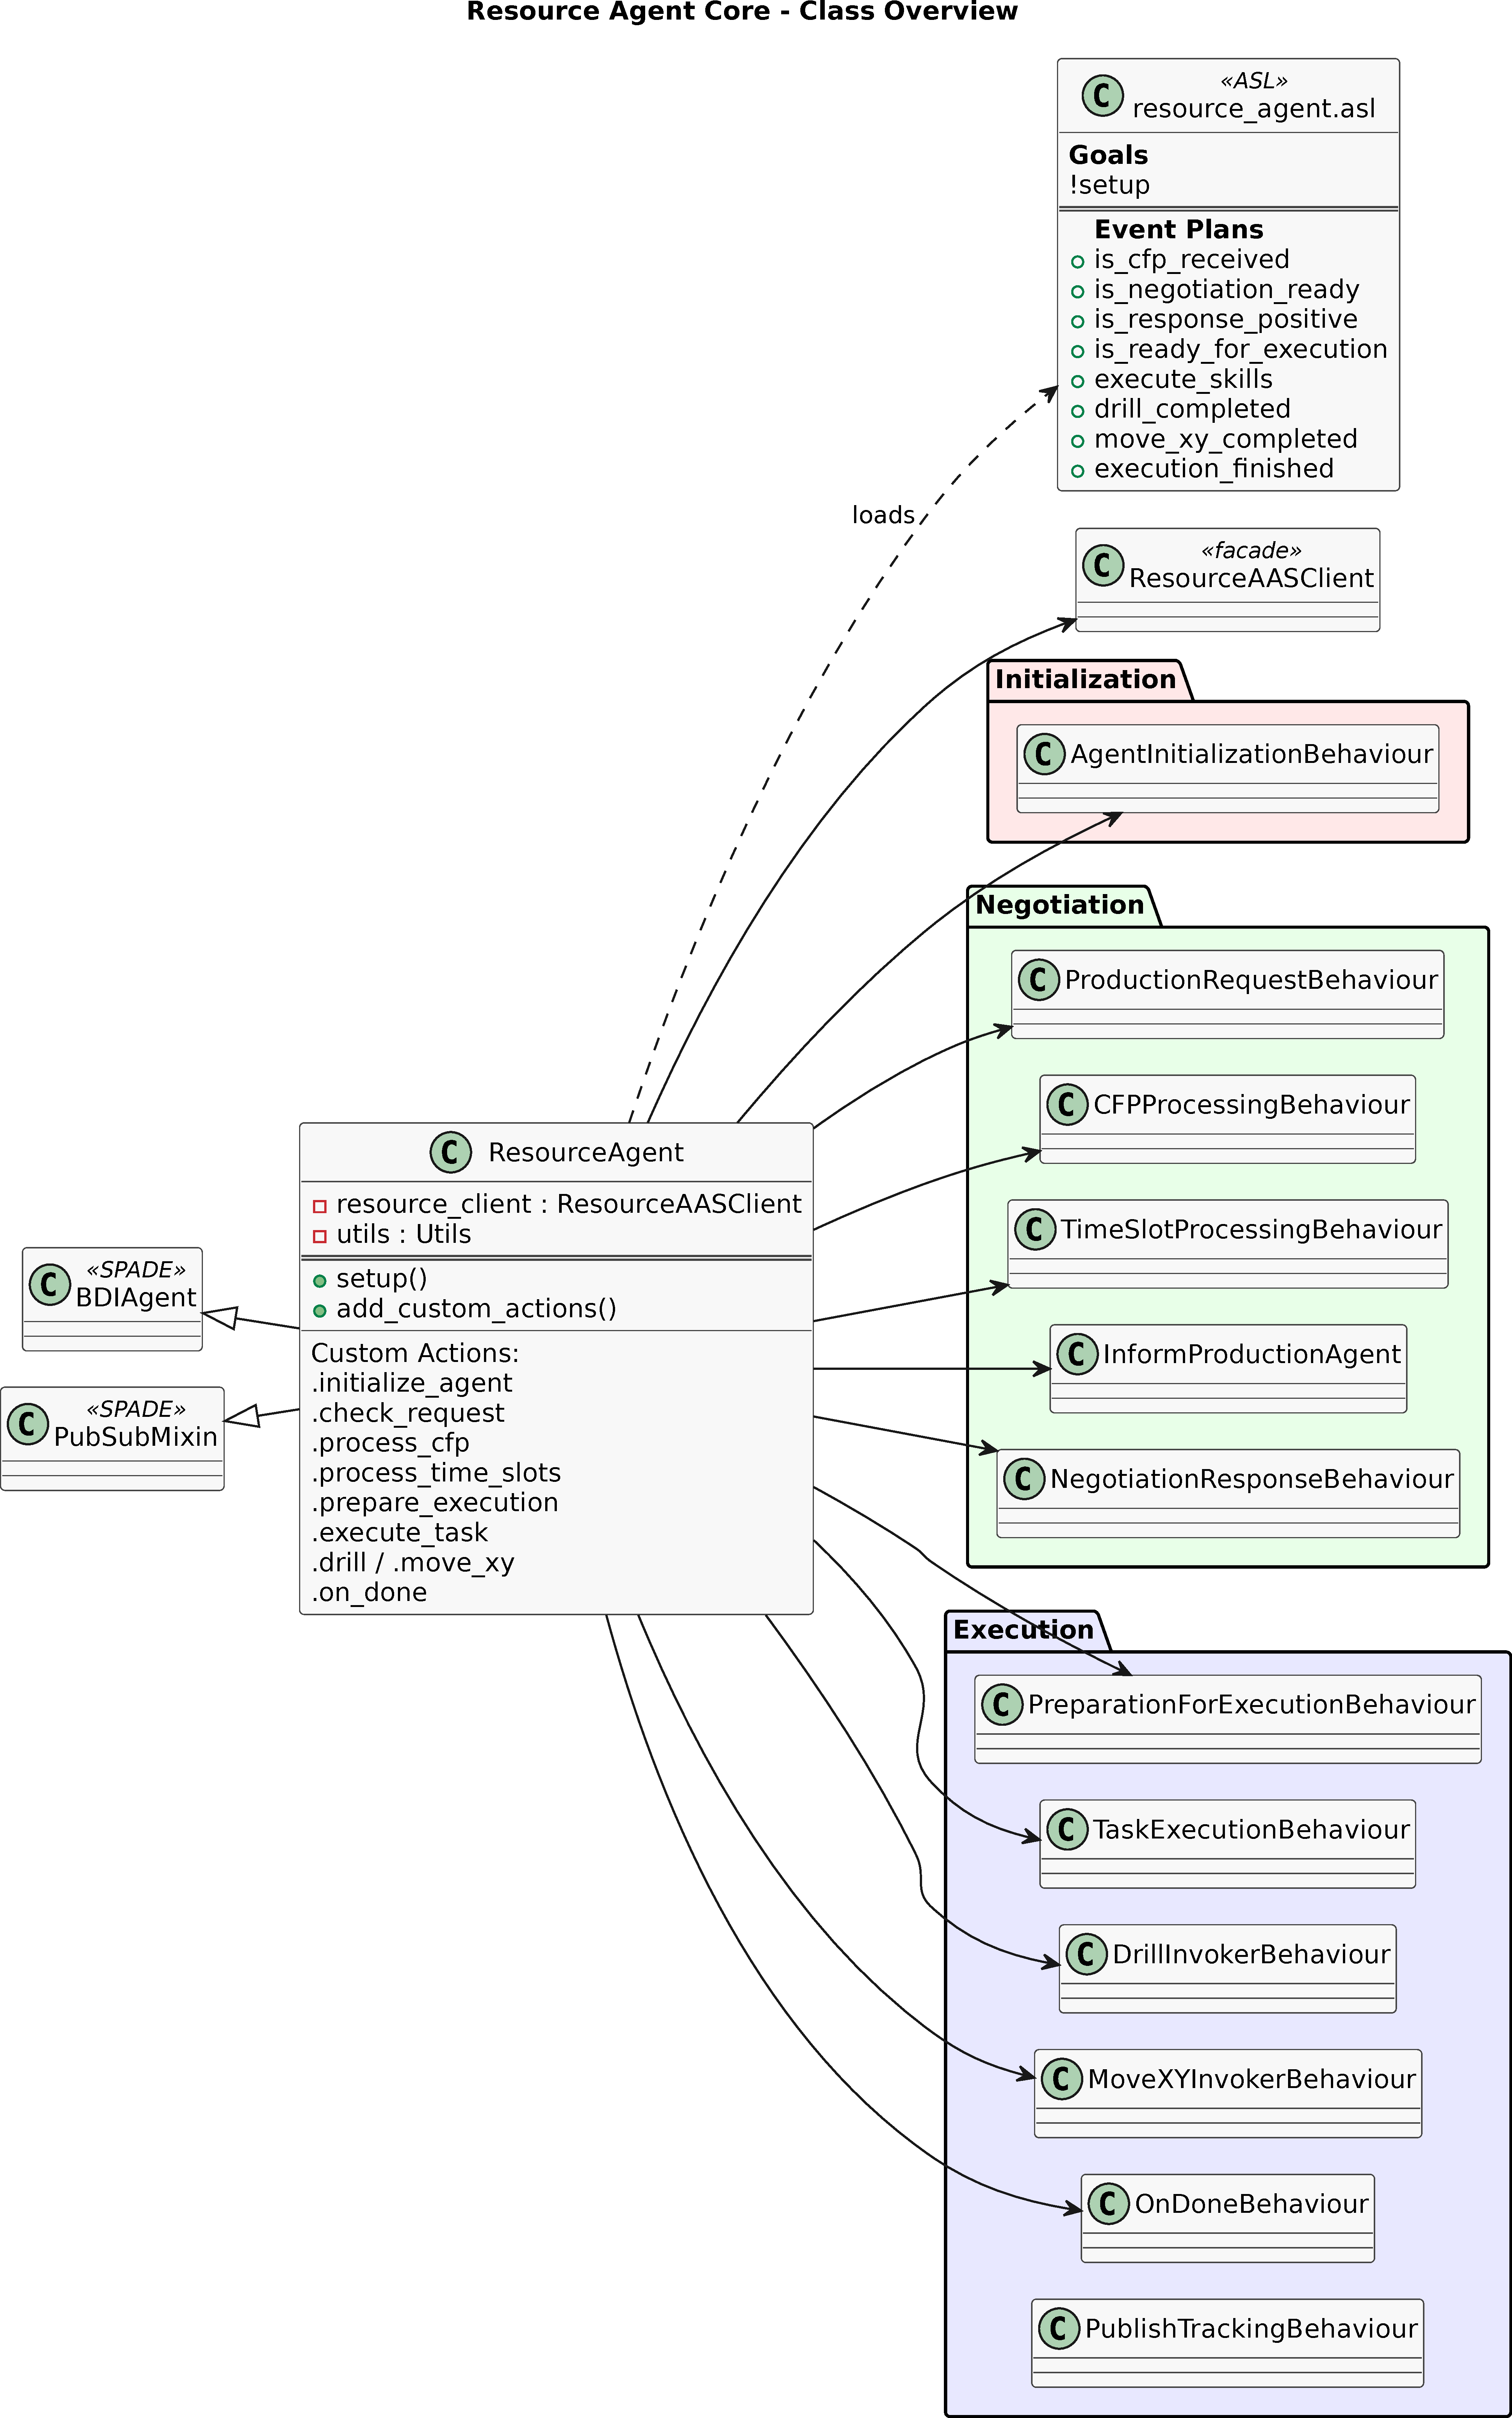
\includegraphics[width=0.95\textwidth]{Images/Resource_Agent_Core_Simple.pdf}
    \caption{Resource Agent Core Class Architecture}
    \label{fig:resource_agent_core}
\end{figure}

\subsubsection{ResourceAgent Class}

The \texttt{ResourceAgent} class extends both \texttt{BDIAgent} and \texttt{PubSubMixin} from the SPADE framework. This dual inheritance combines AgentSpeak-based reasoning with \ac{XMPP} publish-subscribe messaging. The agent maintains a reference to the \texttt{ResourceAASClient} for \ac{AAS} communication and registers custom actions that map AgentSpeak plan actions to SPADE behaviors.

Custom actions are registered in the \texttt{add\_custom\_actions()} method. Each action corresponds to a specific behavior class. For example, when an AgentSpeak plan executes \texttt{.drill}, the agent instantiates and adds a \texttt{DrillInvokerbehavior} to its execution queue.
\subsubsection{AgentSpeak Plans}

The agent's reactive behavior is defined in the \texttt{resource\_agent.asl} file using AgentSpeak syntax. Plans follow the pattern \texttt{+trigger : context <- body}, where the trigger is a belief change, the context is an optional condition, and the body contains actions to execute.

\textbf{Initialization.} The agent starts with the goal \texttt{!setup}, which triggers belief loading from \ac{AAS} submodels and initiates request listening.

\textbf{Negotiation Plans.} When a Call-For-Proposal arrives, the belief \texttt{is\_cfp\_received(true)} triggers validation plans that check time slots, current state, and skill constraints. The result is published back to the ProductionAAS.

\textbf{Execution Plans.} Upon receiving a positive negotiation response, execution plans coordinate the operation sequence. For drilling tasks, the agent first executes \texttt{move\_xy}, then upon completion triggers \texttt{drill}. Context conditions ensure correct sequencing:
\begin{verbatim}
+move_xy_completed(true) : current_operation(drill) <-
    .drill.
\end{verbatim}
\subsubsection{SPADE behaviors}

behaviors implement the actual logic for each agent action. They are organized into three categories:

\textbf{Initialization behaviors.} \texttt{AgentInitializationbehavior} reads beliefs from all four submodels concurrently using \texttt{asyncio.gather()}, populating the agent's belief base with current state, supported skills, constraints, and time slot availability.

\textbf{Negotiation behaviors.} These behaviors handle the Contract Net Protocol interaction:
\begin{itemize}
    \item \texttt{ProductionRequestbehavior}: Listens for CFP messages via \ac{XMPP} PubSub
    \item \texttt{TimeSlotProcessingbehavior}: Validates requested time slot availability
    \item \texttt{CFPProcessingbehavior}: Validates state, skills, and constraints against the CFP
    \item \texttt{InformProductionAgent}: Sends the negotiation response with any violations
    \item \texttt{NegotiationResponsebehavior}: Processes the ProductionAAS decision
\end{itemize}

\textbf{Execution behaviors.} These behaviors execute the actual operations:
\begin{itemize}
    \item \texttt{PreparationForExecutionbehavior}: Prepares the resource (e.g., allocates time slot)
    \item \texttt{TaskExecutionbehavior}: Determines which skill to execute based on the CFP
    \item \texttt{DrillInvokerbehavior}: Invokes the drill operation via the \ac{AAS} API
    \item \texttt{MoveXYInvokerbehavior}: Invokes the positioning operation
    \item \texttt{PublishTrackingbehavior}: Publishes execution status events
    \item \texttt{OnDonebehavior}: Performs cleanup and releases allocated resources
\end{itemize}


\subsubsection{Agent State Machine}

Figure~\ref{fig:resource_agent_statemachine} shows the complete state machine of the ResourceAgent, illustrating the flow from initialization through negotiation to execution.

\begin{figure}[p]
    \centering
    \makebox[\textwidth][c]{%
        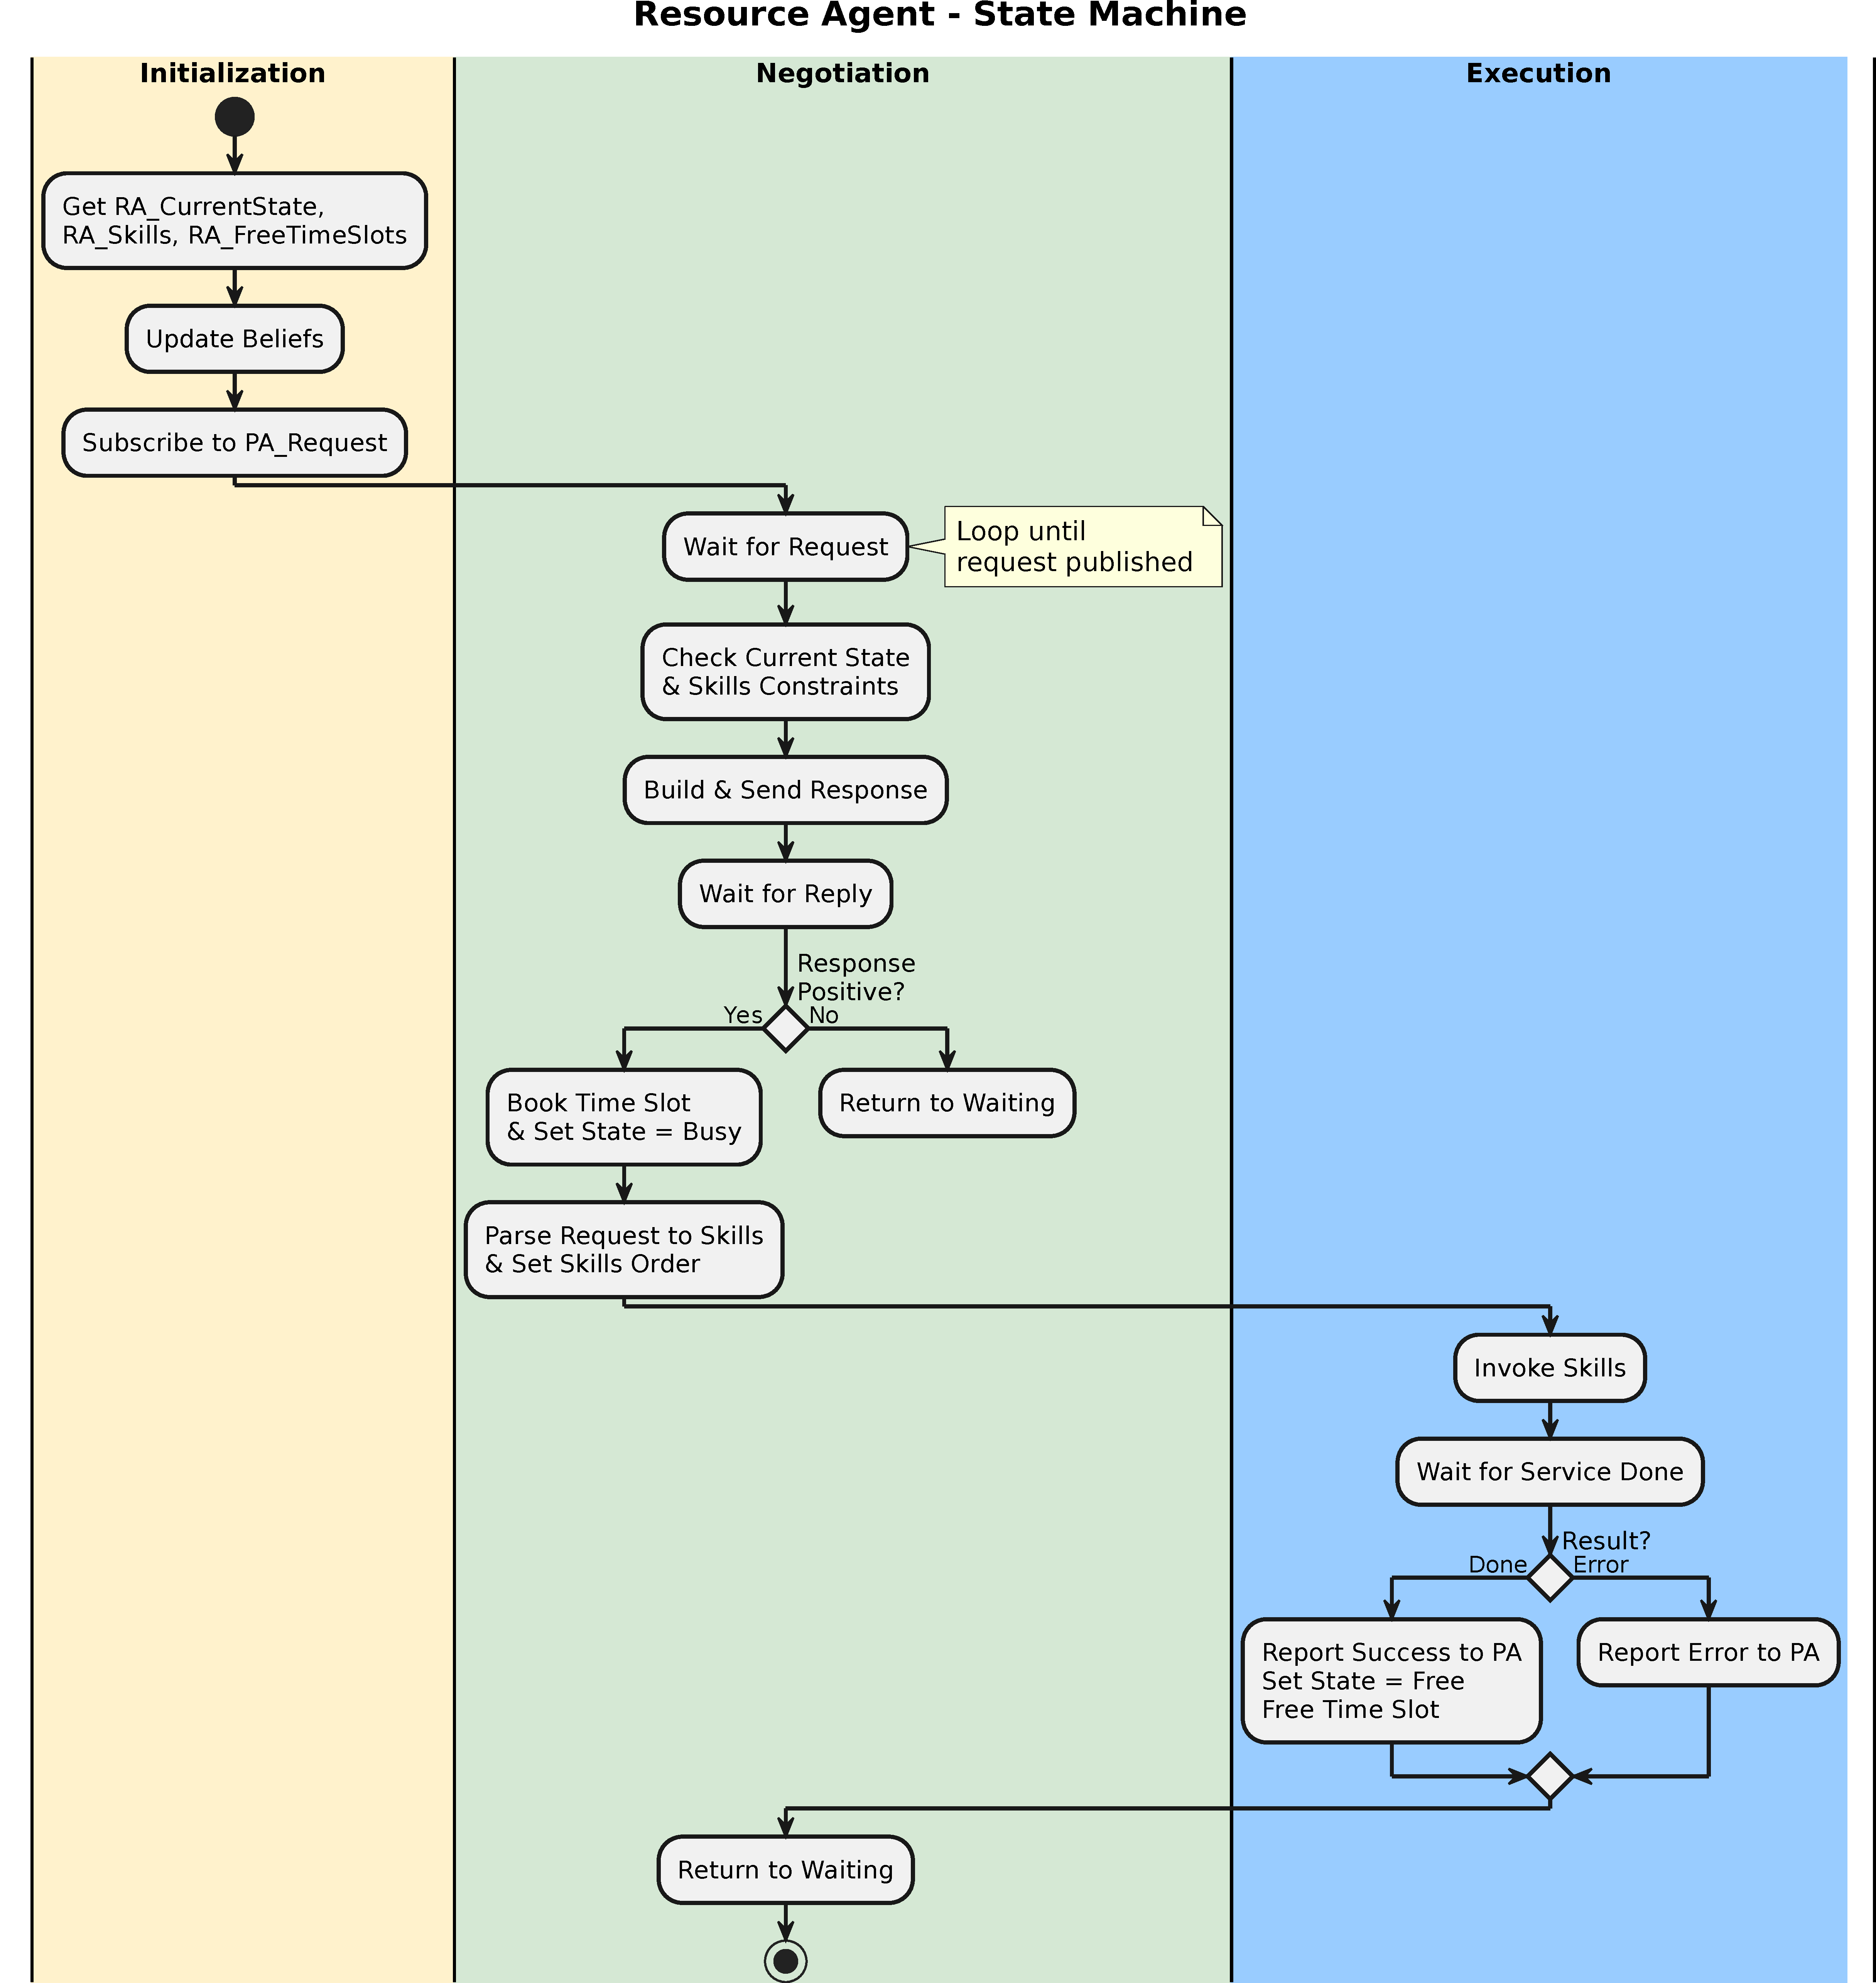
\includegraphics[width=1.3\textwidth]{Images/Resource_Agent_State_Machine.pdf}%
    }
    \caption{Resource Agent State Machine}
    \label{fig:resource_agent_statemachine}
\end{figure}
The state machine comprises six main phases: initialization (loading beliefs from submodels), waiting (listening for CFP requests), CFP processing (validating the request), negotiation response handling (waiting for ProductionAAS decision), execution (performing the requested operation), and cleanup (releasing resources and returning to waiting state).

\subsection{Resource Simulators}
\label{subsec:resource_simulators}
To enable testing and validation of the ResourceAAS without physical hardware, the system includes discrete-event simulators that emulate the behavior of drill machines and positioning systems. These simulators implement the same HTTP endpoints as real machine controllers, allowing seamless integration with the \ac{AAS} infrastructure via the invocationDelegation pattern.

\subsubsection{Simulator Architecture}

Each simulator is implemented as a standalone FastAPI application that combines discrete-event simulation with asynchronous HTTP handling. The architecture uses SimPy~\cite{simpy}, a process-based discrete-event simulation framework for Python, to model machine operations with realistic timing behavior. Figure~\ref{fig:simulator_architecture} illustrates the simulator integration.

\begin{figure}[ht]
    \centering
    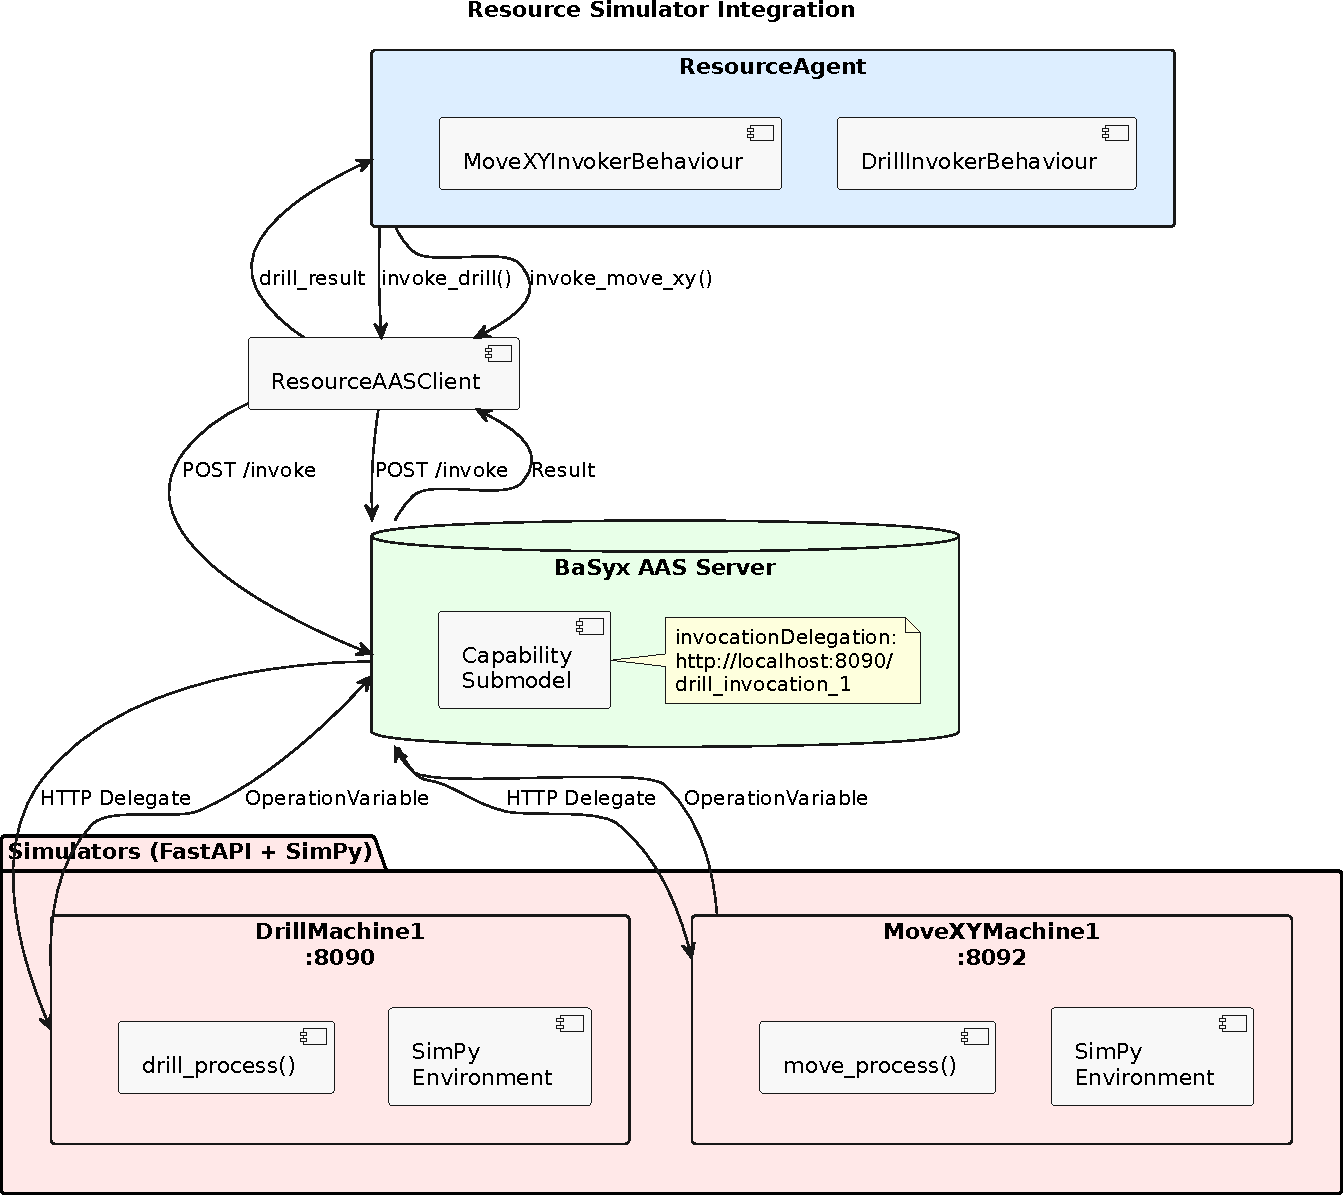
\includegraphics[width=0.95\textwidth]{Images/simulator_architecture.pdf}
    \caption{Resource Simulator Integration Architecture}
    \label{fig:simulator_architecture}
\end{figure}

The simulators expose HTTP endpoints that match the invocationDelegation URLs defined in the Capability Submodel Operations. When the BaSyx server receives an operation invocation request, it forwards the call to the simulator endpoint, which executes the simulated operation and returns \ac{AAS}-compliant results.
\subsubsection{Drill Machine Simulator}

The \texttt{DrillMachine} simulator models drilling operations with configurable speed factors and setup times. Key components include:

\textbf{Machine State.} The simulator maintains state information including current operational status (Idle/Drilling), last drill depth, jobs completed, and cumulative drill time.

\textbf{Drill Process.} The SimPy process calculates drill duration based on depth and RPM parameters using a simple simulation formula:
\begin{equation}
t_{drill} = t_{setup} + depth \times factor_{speed} \times \frac{1500}{RPM}
\end{equation}
This formula scales drill time linearly with depth and inversely with RPM, plus a fixed setup time. It is not based on real machining physics but provides a reasonable approximation for simulation purposes, where higher RPM values result in faster drilling and deeper holes require proportionally more time.

\textbf{Resource Management.} A SimPy Resource with capacity 1 ensures mutual exclusion, preventing concurrent operations on the same machine.

\subsubsection{MoveXY Simulator}

The \texttt{MoveXYMachine} simulator models 2D positioning operations. It tracks the current position and calculates movement time based on Euclidean distance:
\begin{equation}
t_{move} = t_{setup} + \sqrt{(x_{target} - x_{current})^2 + (y_{target} - y_{current})^2} \times factor_{move}
\end{equation}
Similar to the drill formula, this is a simplified simulation model where movement time scales linearly with distance traveled, plus a fixed setup time. The simulator maintains position state between operations, enabling realistic simulation of sequential movements.

\subsubsection{AAS Integration}

Simulators integrate with the \ac{AAS} infrastructure through the invocationDelegation pattern:

\begin{enumerate}
    \item The ResourceAgent behavior calls \texttt{invoke\_drill()} on the ResourceAASClient
    \item The client sends an invocation request to the BaSyx server
    \item BaSyx reads the invocationDelegation qualifier from the Operation element
    \item BaSyx forwards the request to the simulator endpoint\\
    (e.g., \texttt{http://localhost:8090/drill\_invocation\_1})
    \item The simulator executes the SimPy process and returns \ac{AAS}-compliant OperationVariable results
    \item The response propagates back through BaSyx to the agent
\end{enumerate}

This design enables transparent switching between simulators and real machine controllers by modifying only the invocationDelegation URL in the Capability Submodel, without changes to agent code.

\subsubsection{Simulator Instances}

The system includes four simulator instances to support the multi-resource scenario:

\begin{table}[ht]
\centering
\caption{Resource Simulator Configuration}
\label{tab:simulator_config}
\begin{tabular}{llll}
\toprule
\rowcolor{headerblue}
\textcolor{white}{Simulator} & \textcolor{white}{Port} & \textcolor{white}{Endpoint} & \textcolor{white}{Resource} \\
\midrule
DrillMachine1 & 8090 & /drill\_invocation\_1 & Drill\_1 \\
DrillMachine2 & 8091 & /drill\_invocation\_2 & Drill\_2 \\
MoveXYMachine1 & 8092 & /movexy\_invocation\_1 & Drill\_1 \\
MoveXYMachine2 & 8093 & /movexy\_invocation\_2 & Drill\_2 \\
\bottomrule
\end{tabular}
\end{table}

Each drill machine resource has an associated MoveXY simulator, reflecting the physical configuration where positioning and drilling are separate actuators on the same machine.


\section{Production Agent Concept}
\label{sec:production_agent}

The ProductionAAS orchestrates the manufacturing process by coordinating resource agents, managing process plans, and tracking execution progress. Unlike the ResourceAAS which represents physical assets, the ProductionAAS operates at the product level, initiating negotiations with resources and monitoring task completion. This section describes the Production Agent architecture, submodels, and its dual-core design for execution and negotiation.

\subsection{Production Agent Overview}
\label{subsec:production_overview}

The ProductionAAS follows a similar architectural pattern to the ResourceAAS but serves a different purpose in the system hierarchy. While ResourceAAS agents represent manufacturing capabilities, the ProductionAAS represents production orders and coordinates the execution of process plans across multiple resources. Figure~\ref{fig:production_components} illustrates the Production Agent component structure.
\begin{figure}[p]
    \centering
    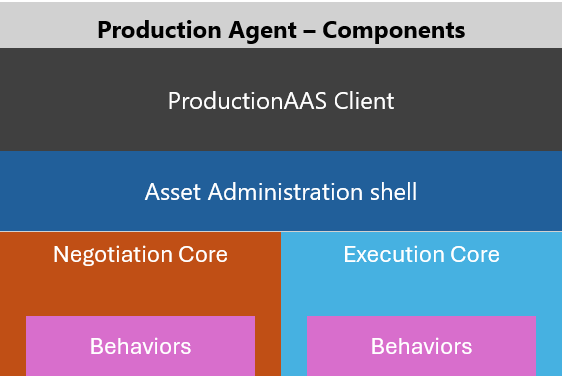
\includegraphics[width=0.9\textwidth]{Images/production_components.png}
    \caption{Production Agent Component Structure}
    \label{fig:production_components}
\end{figure}

\textbf{ProductionAASClient.} Similar to the ResourceAASClient, this facade aggregates repository classes for accessing Production submodels. It provides methods for reading process plans, updating execution state, and managing interface configurations.


\textbf{Asset Administration Shell.} The Production \ac{AAS} contains submodels that describe the production order rather than physical capabilities. These include the Process Plan defining the sequence of operations, Execution Tracking for monitoring progress, and Interface Endpoints for communication configuration. The shell is deployed to the same BaSyx environment as ResourceAAS instances, enabling unified access through the \ac{AAS} API.

\textbf{Dual-Core Agent Architecture.} The Production Agent implements a separation of concerns through two specialized agent cores:
\begin{itemize}
    \item \textbf{Execution Core}: Handles user requests, monitors execution progress, and updates the Execution Tracking submodel based on events from resource agents.
    \item \textbf{Negotiation Core}: Manages the Contract Net Protocol interaction with resource agents, collecting responses and selecting the best-fit resource for task execution.
\end{itemize}

This separation allows independent scaling and clearer responsibility boundaries compared to a monolithic agent design.
\begin{figure}[p]
    \centering
    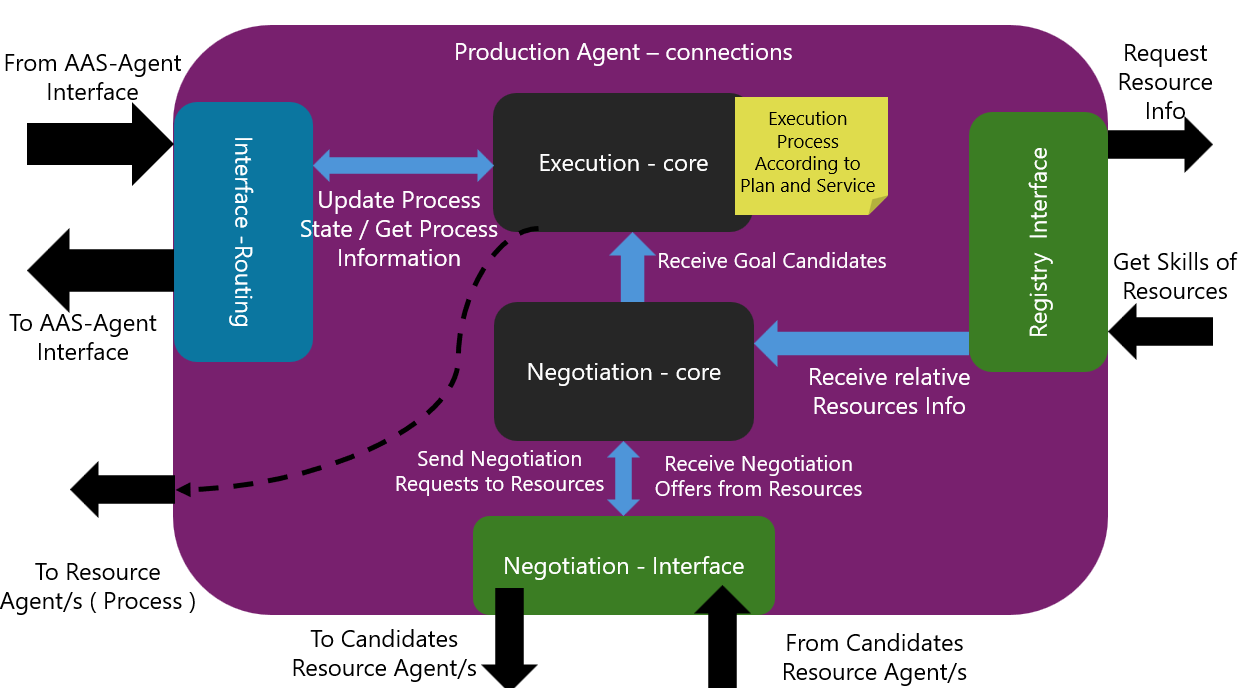
\includegraphics[width=0.9\textwidth]{Images/production_Internal.png}
    \caption{Production Agent Internal Architecture}
    \label{fig:production_internal}
\end{figure}


\subsection{Production Agent Submodels}
\label{subsec:production_submodels}
The ProductionAAS contains three submodels that support process definition, execution monitoring, and communication configuration.

\subsubsection{Process Plan Submodel}

The Process Plan Submodel defines the sequence of operations required to fulfill a production order. It uses a graph-based representation with nodes, edges, and control flow elements. Figure~\ref{fig:sm_process_plan} shows the structure of this submodel.

\textbf{Nodes.} A SubmodelElementCollection containing Property elements for each operation in the process. In the drill machine scenario, this includes:
\begin{itemize}
    \item \texttt{Move\_Node}: Positioning operation to coordinates X, Y
    \item \texttt{Drill\_Node}: Drilling operation with depth and RPM parameters
\end{itemize}

\textbf{Edges.} A SubmodelElementCollection defining the execution sequence between nodes (e.g., ``Move\_Node to Drill\_Node'').

\textbf{Entry\_Point / Exit\_Point.} Properties indicating the first and last nodes in the process plan, enabling the Execution Core to determine where to begin and when execution is complete.

\textbf{Preconditions / Postconditions.} Properties defining the required state before execution can begin and the expected state after completion.

\textbf{Required\_Capabilities.} A list of capabilities needed to execute the process plan (e.g., ``[Drill\_Capability, MoveXY\_Capability]''). The Negotiation Core uses this to filter resource agents during CFP broadcast.


\begin{landscape}
\begin{figure}[p]
    \centering
    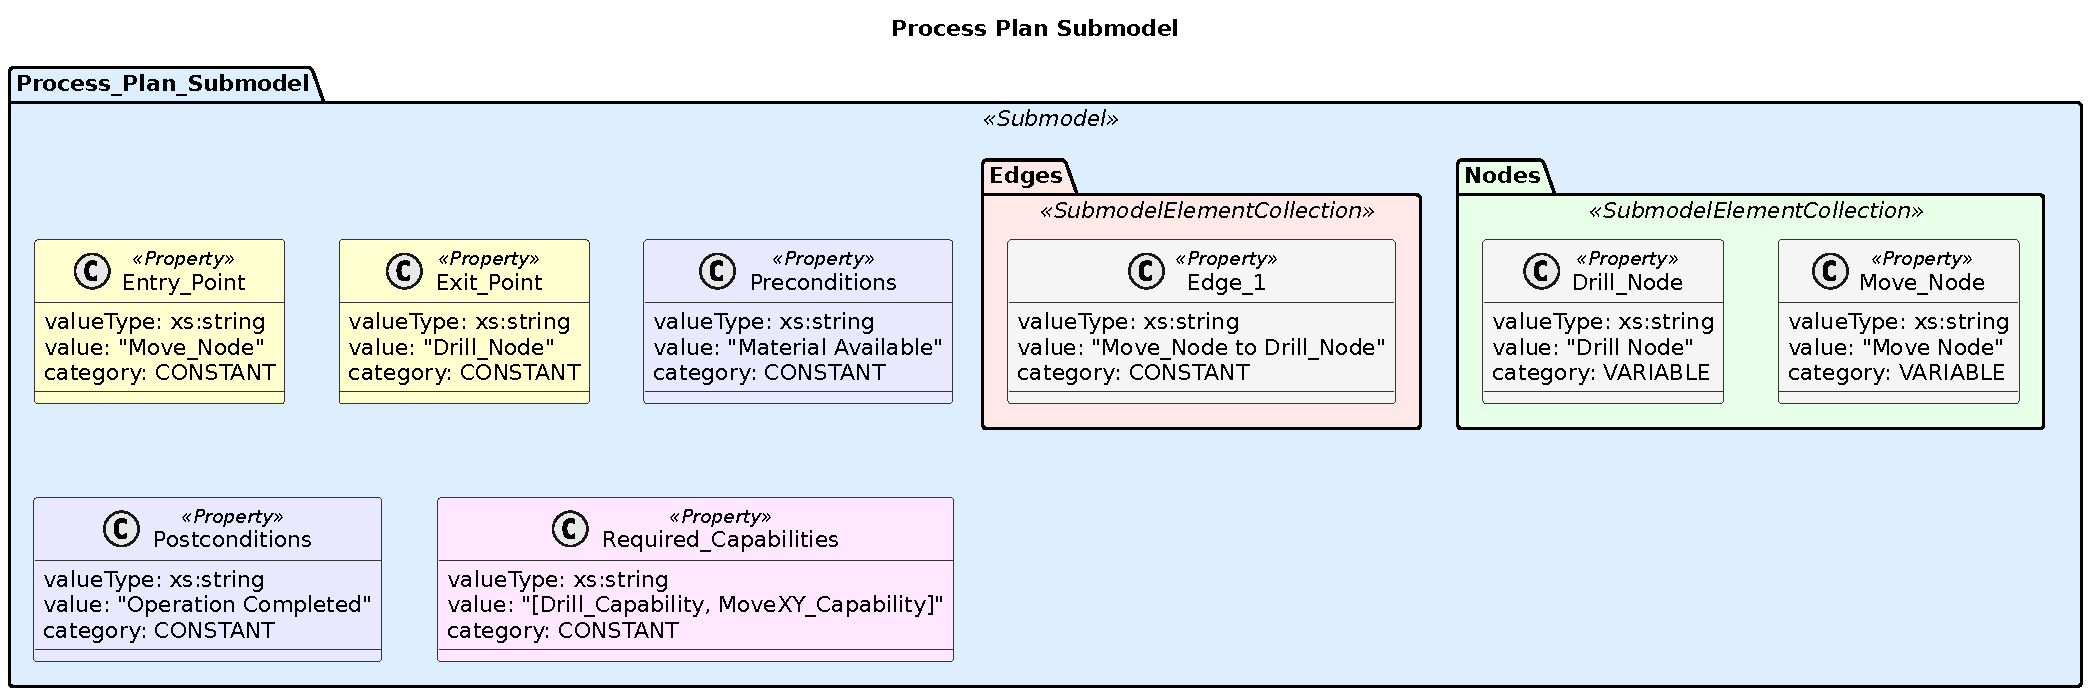
\includegraphics[width=24cm]{Images/sm_process_plan.pdf}
    \caption{Process Plan Submodel Structure}
    \label{fig:sm_process_plan}
\end{figure}
\end{landscape}
\subsubsection{Execution Tracking Submodel}

The Execution Tracking Submodel provides real-time visibility into process execution. It is updated by the Execution Core as resource agents report progress. Figure~\ref{fig:sm_execution_tracking} shows the structure.

\begin{figure}[p]
    \centering
    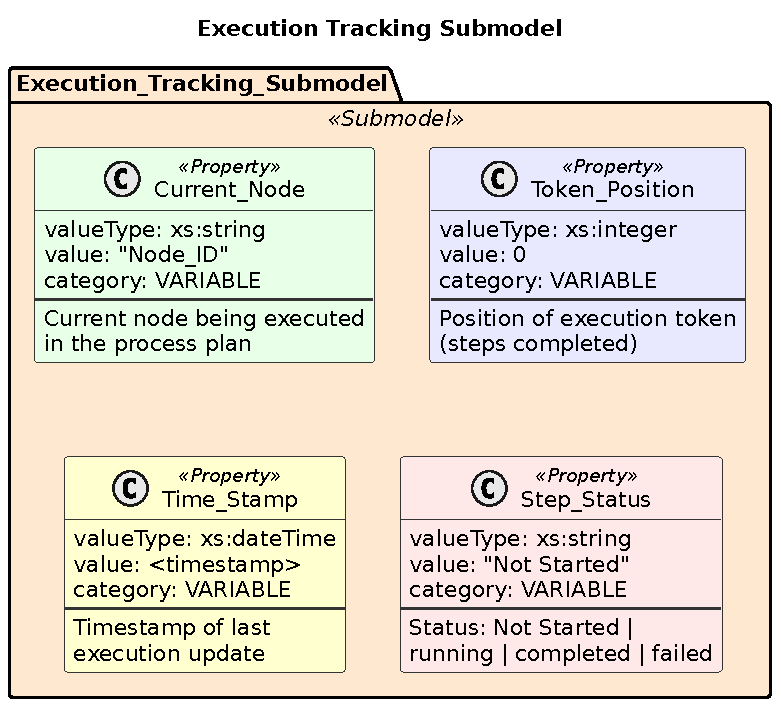
\includegraphics[width=0.9\textwidth]{Images/sm_execution_tracking.pdf}
    \caption{Execution Tracking Submodel Structure}
    \label{fig:sm_execution_tracking}
\end{figure}

\textbf{Current\_Node.} The node currently being executed in the process plan, updated when resource agents publish tracking events.

\textbf{Token\_Position.} An integer indicating how many steps have been completed, implementing a simple Petri net-style token tracking mechanism.

\textbf{Time\_Stamp.} The timestamp of the last execution update, providing temporal context for monitoring systems.

\textbf{Step\_Status.} The status of the current operation: ``Not Started'', ``running'', ``completed'', or ``failed''.

\subsubsection{Interface Endpoints Submodel}

The Interface Endpoints Submodel as in figure~\ref{fig:sm_interface_endpoints} contains configuration for external communication, similar to the Interaction Submodel in ResourceAAS but focused on command invocation endpoints.

\begin{figure}[p]
    \centering
    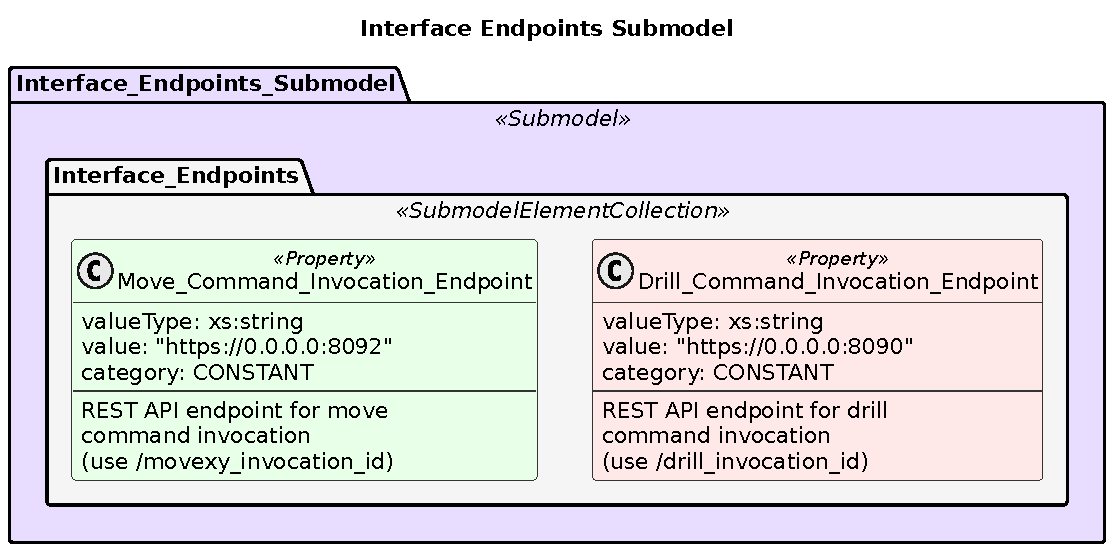
\includegraphics[width=0.9\textwidth]{Images/sm_interface_endpoints.pdf}
    \caption{Interface Endpoints Submodel Structure}
    \label{fig:sm_interface_endpoints}
\end{figure}

\textbf{Endpoints Collection.} Contains properties for:
\begin{itemize}
    \item \texttt{Drill\_Command\_Invocation\_Endpoint}: Base URL for drill operation invokers
    \item \texttt{Move\_Command\_Invocation\_Endpoint}: Base URL for movement operation invokers
\end{itemize}




\subsection{Production Agent Execution Core}
\label{subsec:production_execution}

The Execution Core manages the lifecycle of production requests from receipt through completion. It operates as a SPADE agent extending both \texttt{Agent} and \texttt{PubSubMixin} for \ac{XMPP} communication. Figure~\ref{fig:execution_core} illustrates the class architecture.

\begin{landscape}
    

\begin{figure}[p]
    \centering
    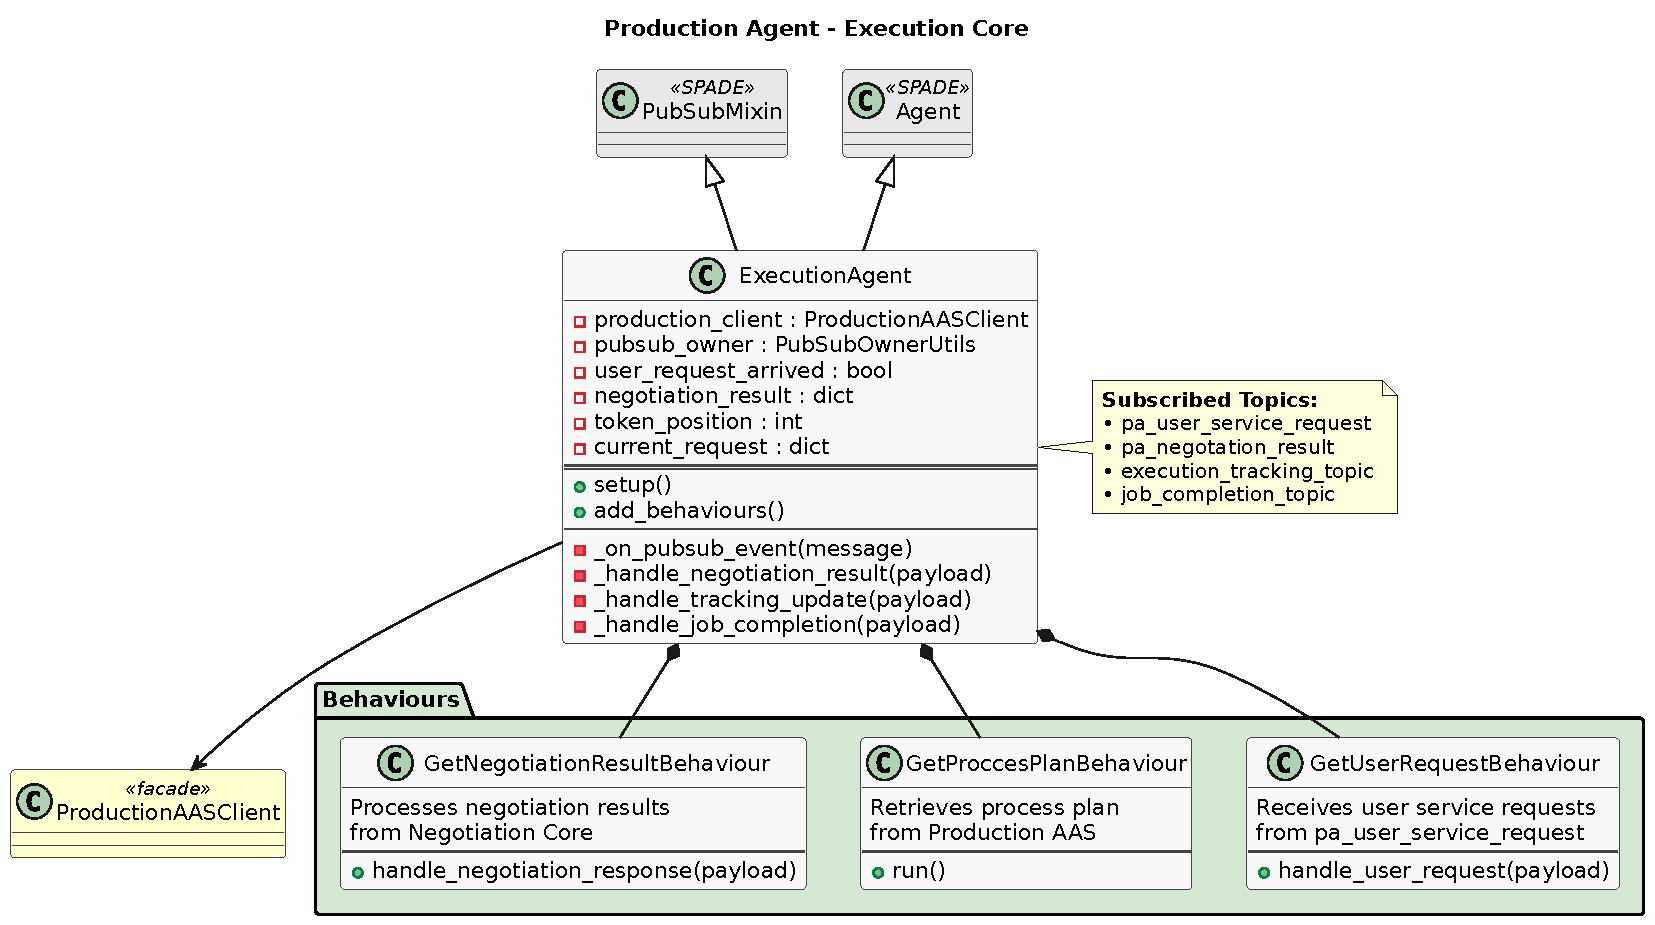
\includegraphics[width=24cm]{Images/execution_core_simple.pdf}
    \caption{Execution Core Class Architecture}
    \label{fig:execution_core}
\end{figure}
\end{landscape}
\subsubsection{ExecutionAgent Class}

The \texttt{ExecutionAgent} class serves as the central coordinator for production execution. It maintains several key attributes:

\begin{itemize}
    \item \texttt{production\_client}: Reference to the ProductionAASClient for accessing submodel data
    \item \texttt{pubsub\_owner}: Utility for managing \ac{XMPP} PubSub node ownership and subscriptions
    \item \texttt{negotiation\_result}: Stores the selected resource and parameters from negotiation
    \item \texttt{token\_position}: Tracks execution progress through the process plan (Petri net-style counter)
    \item \texttt{current\_request}: Stores the active production request for reference during tracking
\end{itemize}

During setup, the agent initializes the ProductionAASClient and subscribes to four \ac{XMPP} topics:
\begin{itemize}
    \item \texttt{pa\_user\_service\_request}: Receives new production requests
    \item \texttt{pa\_negotation\_result}: Receives negotiation outcomes from the Negotiation Core
    \item \texttt{execution\_tracking\_topic}: Receives progress updates from resource agents
    \item \texttt{job\_completion\_topic}: Receives task completion notifications
\end{itemize}

\subsubsection{Event Handling}

The \texttt{\_on\_pubsub\_event()} method routes incoming messages to appropriate handlers based on the topic:

\textbf{User Request Handling.} When a message arrives on \texttt{pa\_user\_service\_request}, the agent delegates to \texttt{GetUserRequestbehavior}, which parses the CFP message and forwards it to the Negotiation Core.

\textbf{Negotiation Result Handling.} The \texttt{\_handle\_negotiation\_result()} method processes the selected resource information, logs the negotiation summary, and triggers execution preparation.

\textbf{Tracking Update Handling.} The \texttt{\_handle\_tracking\_update()} method receives progress events from resource agents during execution. For each update, it increments the token position, updates the Execution Tracking Submodel via the ProductionAASClient, and logs the operation status.

\textbf{Job Completion Handling.} The \texttt{\_handle\_job\_completion()} method finalizes the production run by logging completion status and saving execution reports.

\subsubsection{behaviors}

The Execution Core uses three behaviors to handle different aspects of request processing:

\textbf{GetUserRequestbehavior.} Receives and parses user service requests from the \texttt{pa\_user\_service\_request} topic. It extracts the skill requirements, time slot preferences, and input parameters, then publishes the request to the Negotiation Core via \texttt{pa\_execution\_service\_topic}.

\textbf{GetProccesPlanbehavior.} Retrieves the process plan from the Production AAS, providing the Execution Core with information about the sequence of operations, entry/exit points, and required capabilities.

\textbf{GetNegotiationResultbehavior.} Processes negotiation results received from the Negotiation Core. Upon receiving a positive result with a selected resource, it prepares the execution context and waits for tracking updates as the resource agent executes the task.
\subsection{Production Agent Negotiation Core}
\label{subsec:production_negotiation}

The Negotiation Core implements the Contract Net Protocol initiator role, broadcasting Call-For-Proposals to resource agents and selecting the best candidate for task execution. Like the Execution Core, it operates as a SPADE agent with \ac{XMPP} publish-subscribe capabilities. Figure~\ref{fig:negotiation_core} illustrates the class architecture.

\begin{landscape}
\begin{figure}[p]
    \centering
    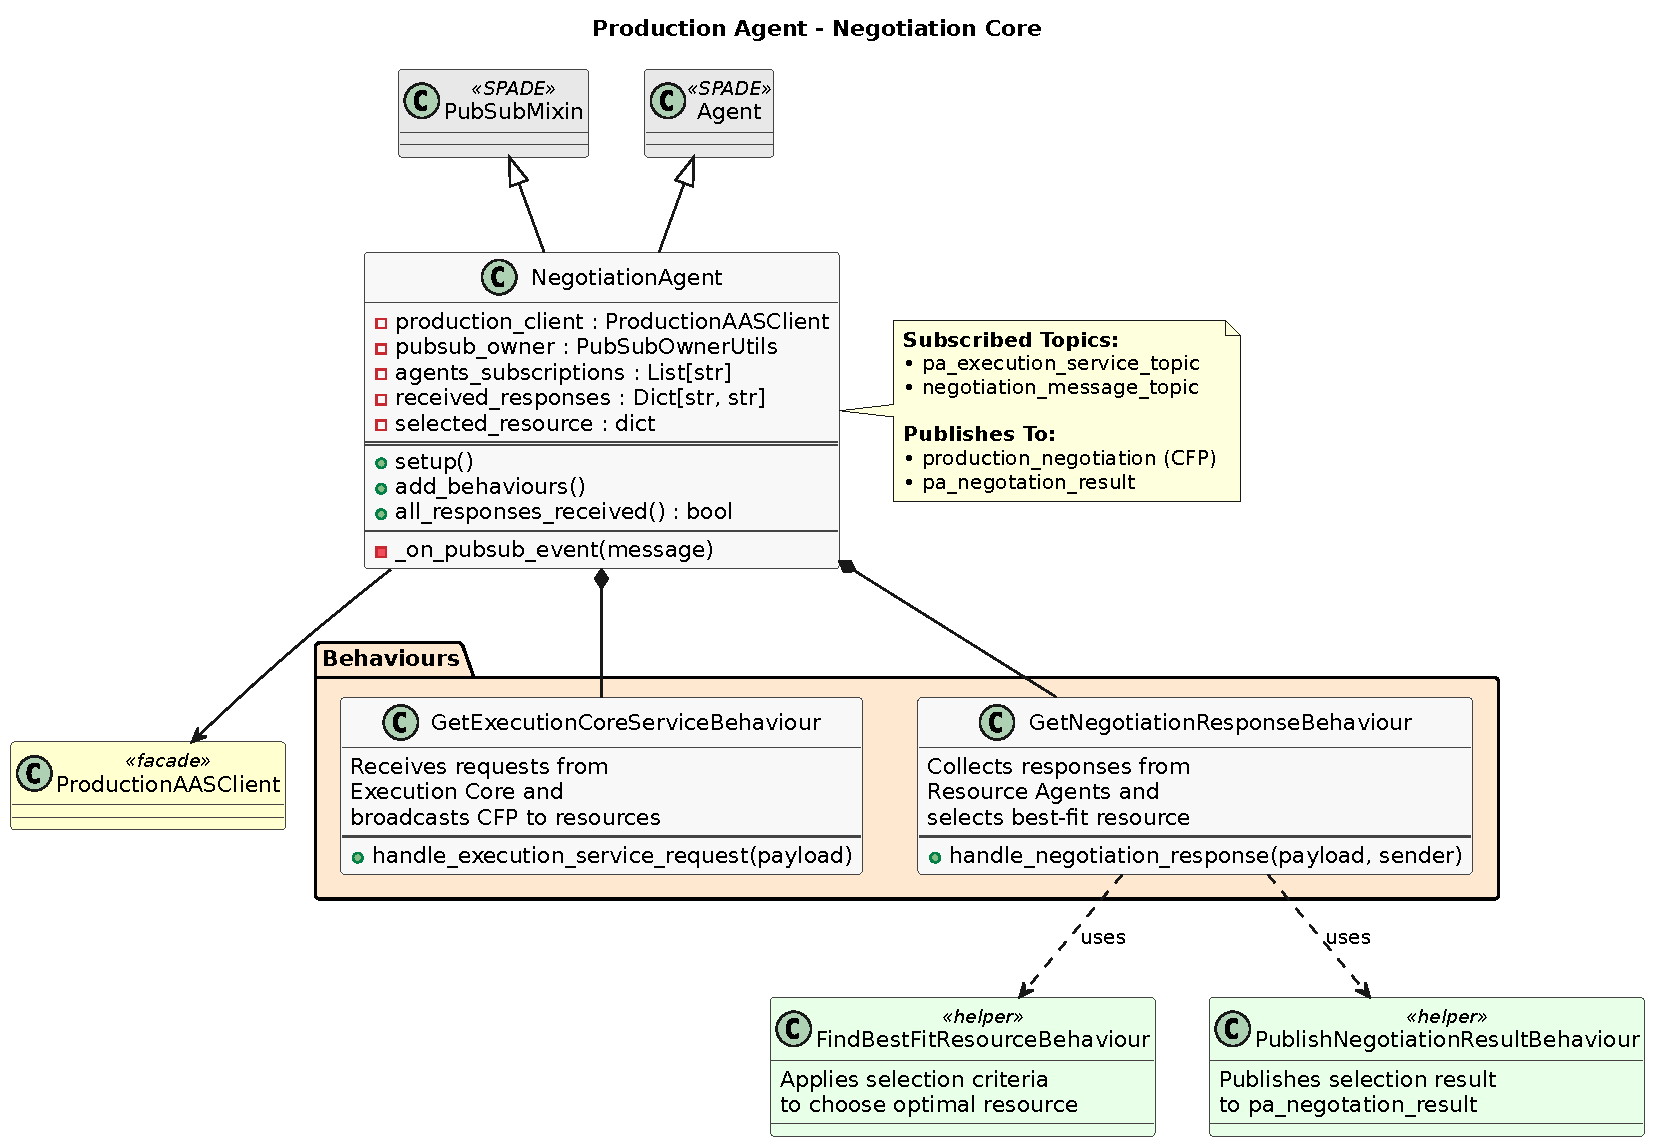
\includegraphics[width=23cm]{Images/negotiation_core_simple.pdf}
    \caption{Negotiation Core Class Architecture}
    \label{fig:negotiation_core}
\end{figure}
\end{landscape}
\subsubsection{NegotiationAgent Class}

The \texttt{NegotiationAgent} class manages the negotiation process with resource agents. It maintains several key attributes:

\begin{itemize}
    \item \texttt{production\_client}: Reference to the ProductionAASClient for accessing submodel data
    \item \texttt{pubsub\_owner}: Utility for querying \ac{XMPP} PubSub node subscribers
    \item \texttt{agents\_subscriptions}: List of resource agent identifiers subscribed to the negotiation topic
    \item \texttt{received\_responses}: Dictionary tracking responses received from each resource agent
    \item \texttt{selected\_resource}: Stores the chosen resource after selection completes
\end{itemize}

During setup, the agent initializes the ProductionAASClient, queries the subscriber list from the \texttt{production\_negotiation} topic, and subscribes to two \ac{XMPP} topics:
\begin{itemize}
    \item \texttt{pa\_execution\_service\_topic}: Receives negotiation requests from the Execution Core
    \item \texttt{negotiation\_message\_topic}: Receives proposal responses from resource agents
\end{itemize}

The agent publishes to:
\begin{itemize}
    \item \texttt{production\_negotiation}: Broadcasts CFP messages to all subscribed resource agents
    \item \texttt{pa\_negotation\_result}: Publishes the selected resource back to the Execution Core
\end{itemize}

\subsubsection{Response Tracking}

The \texttt{all\_responses\_received()} method checks whether all expected resource agents have responded. It compares the set of received response keys against the set of subscribed agents, returning true only when all expected responses have arrived. This ensures the selection algorithm has complete information before making a decision.

\subsubsection{behaviors}

The Negotiation Core uses two main behaviors and two helper behaviors:

\textbf{GetExecutionCoreServicebehavior.} Receives negotiation requests from the Execution Core via \texttt{pa\_execution\_service\_topic}. Upon receiving a request, it:
\begin{enumerate}
    \item Parses the CFP message containing skill requirements and parameters
    \item Broadcasts the CFP to all resource agents via the \texttt{production\_negotiation} topic
    \item Initializes the response tracking dictionary
\end{enumerate}

\textbf{GetNegotiationResponsebehavior.} Collects and processes responses from resource agents. For each incoming response on \texttt{negotiation\_message\_topic}, it:
\begin{enumerate}
    \item Extracts the sender identifier and response payload
    \item Stores the response in the \texttt{received\_responses} dictionary
    \item Checks if all expected responses have been received
    \item When complete, triggers the resource selection process
\end{enumerate}

\textbf{FindBestFitResourcebehavior.} Applies the selection criteria to choose the optimal resource from the collected responses. The selection algorithm:
\begin{enumerate}
    \item Filters out responses with violations (invalid proposals)
    \item Among valid proposals, evaluates based on criteria such as time slot availability
    \item Returns the best-fit resource identifier
\end{enumerate}

\textbf{PublishNegotiationResultbehavior.} Publishes the selection result to \texttt{pa\_negotation\_result}, informing the Execution Core of the chosen resource. The result includes the selected resource identifier, allocated time slot, and original request parameters.

\subsubsection{Contract Net Protocol Flow}

The complete negotiation flow follows the Contract Net Protocol pattern:

\begin{enumerate}
    \item Execution Core publishes a service request to \texttt{pa\_execution\_service\_topic}
    \item Negotiation Core receives the request and broadcasts CFP to \texttt{production\_negotiation}
    \item Resource agents evaluate the CFP against their beliefs and respond with proposals or rejections
    \item Negotiation Core collects all responses via \texttt{negotiation\_message\_topic}
    \item Once all responses are received, the best-fit resource is selected
    \item The selection result is published to \texttt{pa\_negotation\_result}
    \item Execution Core receives the result and monitors execution via tracking topics
\end{enumerate}



\section{System Interaction}
\label{sec:system_interaction}

This section describes the interaction between the Production Agent's dual cores and the Resource Agents during the complete production cycle. The interaction follows a coordinated flow from user request through negotiation to task execution and completion. Figure~\ref{fig:system_interaction} illustrates the complete interaction state machine.

\begin{landscape}
    

\begin{figure}[p]
    \centering
    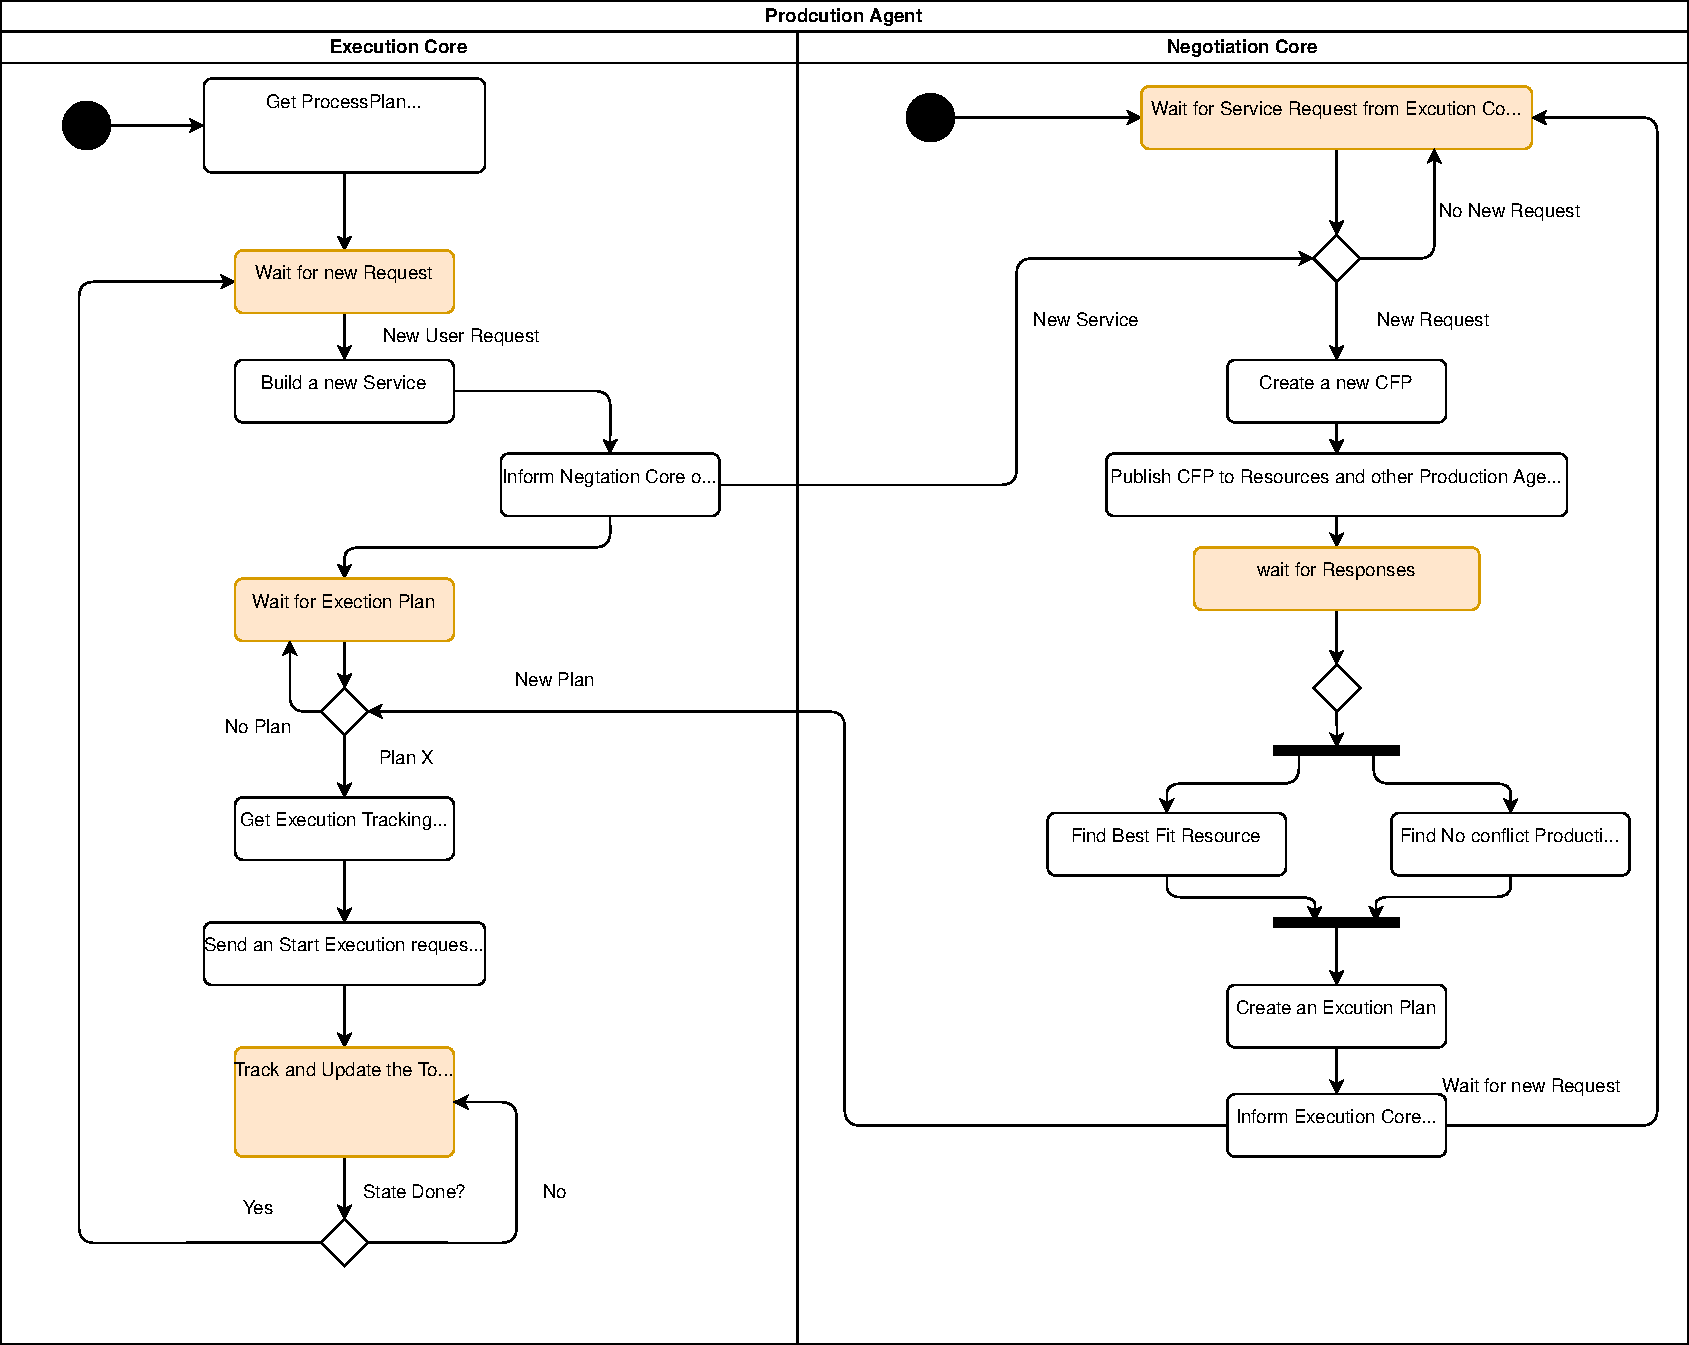
\includegraphics[width=20cm]{Images/PA_SM.pdf}
    \caption{Production Agent - Resource Agent - System Interaction State Machine}
    \label{fig:system_interaction}
\end{figure}
\end{landscape}

\subsection{Execution Core Flow}

The Execution Core operates as the entry point for production requests and manages the overall execution lifecycle:

\textbf{Request Reception.} The flow begins when a user request arrives via the \texttt{pa\_user\_service\_request} topic. The Execution Core receives and parses the request, extracting the required skills, time slot preferences, and input parameters.

\textbf{Service Delegation.} Upon receiving a valid request, the Execution Core publishes a service request to the \texttt{pa\_execution\_service\_topic}, delegating the negotiation task to the Negotiation Core. The Execution Core then enters a waiting state for the negotiation result.

\textbf{Execution Monitoring.} After receiving a positive negotiation result, the Execution Core monitors task execution by subscribing to tracking events from the selected Resource Agent. It updates the Execution Tracking Submodel as operations progress through the process plan.

\textbf{Completion Handling.} When the Resource Agent signals task completion via \texttt{job\_completion\_topic}, the Execution Core finalizes the production run and returns to waiting for the next user request.

\subsection{Negotiation Core Flow}

The Negotiation Core implements the Contract Net Protocol initiator role:

\textbf{CFP Broadcast.} Upon receiving a service request from the Execution Core, the Negotiation Core broadcasts a Call-For-Proposal to all Resource Agents subscribed to the \texttt{production\_negotiation} topic.

\textbf{Response Collection.} The Negotiation Core waits for responses from all subscribed Resource Agents. Each response is stored in a tracking dictionary, and the core checks whether all expected responses have been received.

\textbf{Parallel Response Handling.} Resource Agents respond independently and potentially in parallel. The state machine shows two parallel response paths converging at a synchronization bar, representing the collection of multiple proposals.

\textbf{Resource Selection.} Once all responses are collected, the Negotiation Core applies the best-fit selection algorithm:
\begin{enumerate}
    \item Filter responses without violations (valid proposals)
    \item Evaluate remaining proposals based on selection criteria
    \item Select the optimal resource for task execution
\end{enumerate}

\textbf{Execution Plan Creation.} After selecting a resource, the Negotiation Core creates an execution plan containing the selected resource identifier, allocated time slot, and task parameters.

\textbf{Result Publication.} The Negotiation Core informs the Execution Core of the selection result via \texttt{pa\_negotation\_result} and returns to waiting for the next negotiation request.

\subsection{Inter-Core Communication}

The two cores communicate through \ac{XMPP} publish-subscribe topics, maintaining loose coupling:

\begin{table}[ht]
\centering
\caption{Production Agent Internal Communication Topics}
\label{tab:internal_topics}
\begin{tabular}{lll}
\toprule
\rowcolor{headerblue}
\textcolor{white}{Topic} & \textcolor{white}{Publisher} & \textcolor{white}{Subscriber} \\
\midrule
pa\_execution\_service\_topic & Execution Core & Negotiation Core \\
pa\_negotation\_result & Negotiation Core & Execution Core \\
\bottomrule
\end{tabular}
\end{table}
\subsection{Resource Agent Interaction}

The Production Agent interacts with Resource Agents through external \ac{XMPP} topics:

\begin{table}[ht]
\centering
\caption{Production-Resource Communication Topics}
\label{tab:external_topics}
\begin{tabular}{lll}
\toprule
\rowcolor{headerblue}
\textcolor{white}{Topic} & \textcolor{white}{Direction} & \textcolor{white}{Purpose} \\
\midrule
production\_negotiation & PA → RA & CFP broadcast \\
negotiation\_message\_topic & RA → PA & Proposal responses \\
execution\_tracking\_topic & RA → PA & Progress updates \\
job\_completion\_topic & RA → PA & Task completion \\
\bottomrule
\end{tabular}
\end{table}
This event-driven architecture enables asynchronous coordination between the Production Agent and multiple Resource Agents, supporting scalable multi-resource scenarios without tight coupling between components.

%%%%%%%%%%%%%%%
\section{Submodel Design Considerations}

\label{sec:submodel_design}

This section addresses design decisions and scope limitations of the proposed submodel structures. It differentiates between generic (reusable) and scenario-specific elements, discusses current limitations, and provides guidance for extending the system.
\subsection{Generic vs. Scenario-Specific Elements}
\label{subsec:generic_vs_specific}

The submodel structures are designed with separation between reusable patterns and scenario-specific content. Table~\ref{tab:generic_specific} identifies which elements are transferable to other domains.

\begin{table}[ht]
\centering
\caption{Generic vs. Scenario-Specific Submodel Elements}
\label{tab:generic_specific}
\begin{tabular}{p{0.22\textwidth}p{0.35\textwidth}p{0.33\textwidth}}
\toprule
\rowcolor{headerblue}
\textcolor{white}{Submodel} & \textcolor{white}{Generic (Reusable)} & \textcolor{white}{Scenario-Specific} \\
\midrule
Operational State & Current\_State, Free\_Slots, Booked\_Slots structure & -- \\
\rowcolor{lightgray}
Knowledge & Constraints collection pattern, Constraint\_Type structure & Max\_Depth, Min\_Depth (drilling) \\
Capability & Operation with invocationDelegation, Supported\_Skills list & Drill\_Capability, MoveXY\_Capability \\
\rowcolor{lightgray}
Interaction & Time\_Slots structure, XMPP\_Endpoint & Specific time slot values \\
Process Plan & Nodes, Edges, Entry/Exit\_Point, Required\_Capabilities & Move\_Node, Drill\_Node \\
\rowcolor{lightgray}
Execution Tracking & Current\_Node, Token\_Position, Step\_Status & -- \\
\bottomrule
\end{tabular}
\end{table}
\textbf{Integrating New Resources.} To add a new resource with different capabilities (e.g., a welding machine), the following steps are required:

\begin{enumerate}
    \item \textbf{Define Capability Operations}: Create new \texttt{Operation} elements (e.g., \texttt{Welding\_Capability}) with appropriate input/output parameters and \texttt{invocationDelegation} endpoints.
    
    \item \textbf{Implement Skill Invoker}: Create a simulator or hardware interface that responds to the delegated operation calls.
    
    \item \textbf{Configure Knowledge Constraints}: Define resource-specific constraints (e.g., \texttt{Max\_Weld\_Length}, \texttt{Supported\_Materials}).
    
    \item \textbf{Register Capability String}: Add the capability identifier to \texttt{Supported\_Skills} using the same naming convention.
    
    \item \textbf{Create AgentSpeak Plans}: Add plans for the new skill execution (e.g., \texttt{+excute\_skills(welding\_capability)}).
\end{enumerate}

The submodel \textit{structure} remains unchanged; only the \textit{content} is adapted.
\subsection{Capability Matching Mechanism}
\label{subsec:capability_matching}

The current implementation uses \textbf{string-based capability matching}. The Process Plan specifies required capabilities as strings (e.g., \texttt{"Drill\_Capability"}), and Resource Agents advertise their capabilities in the \texttt{Supported\_Skills} property. During negotiation, string comparison determines compatibility.

\textbf{Limitation}: This approach is susceptible to errors:
\begin{itemize}
    \item Typographical errors (e.g., \texttt{"Drill\_Capbility"} vs. \texttt{"Drill\_Capability"})
    \item Inconsistent naming conventions across resources
    \item No semantic understanding of capability equivalence
\end{itemize}

\textbf{Recommended Extension}: Future implementations should adopt a formal capability ontology or taxonomy. Options include:
\begin{itemize}
    \item \textbf{ECLASS}: Standardized classification for products and services
    \item \textbf{IEC CDD}: Common Data Dictionary for industrial terminology
    \item \textbf{Custom OWL Ontology}: Domain-specific capability definitions with semantic reasoning
\end{itemize}

Using semantic identifiers (IRIs) instead of plain strings would enable:
\begin{itemize}
    \item Capability subsumption (e.g., \texttt{HighSpeedDrilling} is-a \texttt{Drilling})
    \item Equivalence detection across different naming conventions
    \item Automated validation of process plan feasibility
\end{itemize}
\subsection{Process Plan Structure and Limitations}
\label{subsec:process_plan_limitations}

\subsubsection{Linear vs. Precedence Graph Execution}

The current implementation supports \textbf{linear process plans} with sequential node execution. The Process Plan Submodel stores nodes and edges, but the execution logic processes nodes in a fixed sequence (Entry\_Point $\rightarrow$ ... $\rightarrow$ Exit\_Point).

\begin{figure}[ht]
\centering
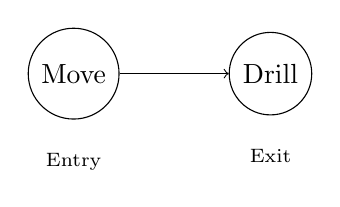
\begin{tikzpicture}[node distance=2.5cm, auto,
    node/.style={circle, draw, minimum size=1cm}]
    \node[node] (A) {Move};
    \node[node, right of=A] (B) {Drill};
    \draw[->] (A) -- (B);
    \node[below=0.3cm of A, font=\scriptsize] {Entry};
    \node[below=0.3cm of B, font=\scriptsize] {Exit};
\end{tikzpicture}
\caption{Current Implementation: Linear Process Plan}
\label{fig:linear_plan}
\end{figure}

\textbf{Limitation}: True precedence graphs with parallel branches are \textbf{not supported} in the current prototype:

\begin{figure}[ht]
\centering
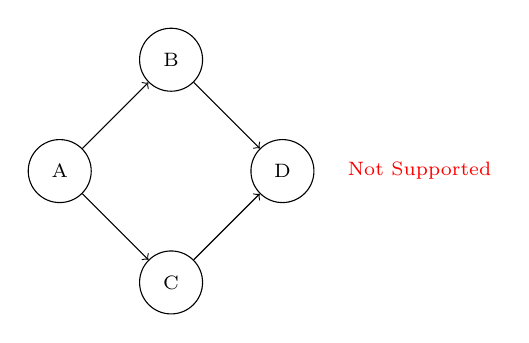
\begin{tikzpicture}[node distance=2cm, auto,
    node/.style={circle, draw, minimum size=0.8cm, font=\scriptsize}]
    \node[node] (A) {A};
    \node[node, above right of=A] (B) {B};
    \node[node, below right of=A] (C) {C};
    \node[node, below right of=B] (D) {D};
    \draw[->] (A) -- (B);
    \draw[->] (A) -- (C);
    \draw[->] (B) -- (D);
    \draw[->] (C) -- (D);
    \node[right=0.3cm of D, font=\scriptsize, text=red] {Not Supported};
\end{tikzpicture}
\caption{Precedence Graph with Parallel Branches (Not Implemented)}
\label{fig:precedence_graph}
\end{figure}

Extending to full precedence graph support would require:
\begin{itemize}
    \item Multiple token positions (see Section~\ref{subsec:token_position})
    \item Fork/join synchronization logic
    \item Parallel resource allocation and negotiation
\end{itemize}
\subsubsection{Capability-Node Association}

In the current design, \texttt{Required\_Capabilities} is a property at the \textbf{Process Plan level}, not associated with individual nodes:

\begin{lstlisting}[language=Python]
sm_required_capabilities = model.Property(
    id_short="Required_Capabilities",
    value="[Drill_Capability, MoveXY_Capability]"  # Plan-level
)
\end{lstlisting}

\textbf{Limitation}: This does not explicitly link which capability is needed for which node. The association is implicit through naming conventions (\texttt{Move\_Node} $\leftrightarrow$ \texttt{MoveXY\_Capability}).

\textbf{Recommended Extension}: Each node should explicitly reference its required capability:

\begin{lstlisting}[language=Python]
sm_move_node = model.SubmodelElementCollection(
    id_short="Move_Node",
    value=[
        model.Property(id_short="Required_Capability", 
                       value="MoveXY_Capability"),
        model.Property(id_short="Sequence_Number", value="1"),
        ...
    ]
)
\end{lstlisting}
\subsection{Token Position and Execution State}
\label{subsec:token_position}

The Execution Tracking Submodel uses a \textbf{single} \texttt{Token\_Position} and \texttt{Current\_Node} property:

\begin{lstlisting}[language=Python]
model.Property(id_short="Token_Position", value="1")
model.Property(id_short="Current_Node", value="Move_Node")
\end{lstlisting}

\textbf{Design Decision}: This models a single execution thread, analogous to a Petri net with one token.

\textbf{Limitation}: In a full Petri net or precedence graph, multiple tokens can exist simultaneously (parallel execution). The current design cannot represent:
\begin{itemize}
    \item Concurrent operations on different resources
    \item Fork states where execution splits
    \item Join states requiring synchronization
\end{itemize}

\textbf{Justification}: For the proof-of-concept with linear plans, a single token is sufficient. Extending to multiple tokens would require refactoring \texttt{Token\_Position} into a collection of token objects.
\subsection{Knowledge Submodel Simplifications}
\label{subsec:knowledge_limitations}

The Knowledge Submodel stores constraints as simple min/max value pairs:

\begin{lstlisting}[language=Python]
model.Property(id_short="Max_Depth", value="100.0")
model.Property(id_short="Min_Depth", value="1.0")
model.Property(id_short="Constraints_Type", value="[Max_Depth, Min_Depth]")
\end{lstlisting}

\textbf{Limitation}: This cannot express \textbf{functional dependencies} between parameters. For example:
\begin{itemize}
    \item A crane's maximum load depends on the boom extension
    \item Drilling speed limits depend on material hardness
    \item Tool wear affects achievable tolerances over time
\end{itemize}

\textbf{Recommended Extension}: Complex constraints could be modeled as:
\begin{itemize}
    \item Mathematical expressions (e.g., \texttt{MaxLoad = f(BoomLength)})
    \item Lookup tables stored as \texttt{SubmodelElementCollection}
    \item References to external constraint models (e.g., FMU/FMI)
\end{itemize}
\subsection{Assembly Processes and Bill of Materials}
\label{subsec:assembly_bom}

The current submodels include a \texttt{Preconditions} property with value \texttt{"Material Available"}, but \textbf{do not model explicit Bill of Materials (BOM)} structures.

\textbf{Scope Limitation}: The proof-of-concept focuses on machining operations (drilling, positioning) where a single workpiece is processed. Assembly scenarios with:
\begin{itemize}
    \item Multiple input parts per operation
    \item Part tracking through production stages
    \item Component-product relationships
\end{itemize}
are \textbf{not covered} by the current submodel design.

\textbf{Extension Approach}: Supporting assembly would require:
\begin{itemize}
    \item BOM Submodel with part references
    \item Material tracking in Operational State
    \item Precondition evaluation logic checking part availability
\end{itemize}
\subsection{User Request Definition}
\label{subsec:user_request}

A \textbf{User Request} is a production order submitted to the Production Agent. In the implementation, it is a message containing:

\begin{table}[ht]
\centering
\caption{User Request Message Structure}
\label{tab:user_request}
\begin{tabular}{lll}
\toprule
\rowcolor{headerblue}
\textcolor{white}{Field} & \textcolor{white}{Type} & \textcolor{white}{Description} \\
\midrule
\texttt{skills\_required} & String & Capability needed (e.g., \texttt{"drill\_capability"}) \\
\texttt{at\_time} & String & Requested time slot (e.g., \texttt{"10:30-11:00"}) \\
\texttt{input\_arguments} & Dictionary & Operation parameters (X, Y, Depth, RPM) \\
\bottomrule
\end{tabular}
\end{table}

The User Request is published to the \texttt{pa\_user\_service\_request} XMPP topic and received by the Execution Core, which initiates the negotiation process.
\subsection{Concrete Example: Drill Operation}
\label{subsec:concrete_example}

To illustrate how the submodels work together, consider a complete drill operation request:

\textbf{Step 1: User Request}
\begin{lstlisting}
{
  "skills_required": "drill_capability",
  "at_time": "10:30-11:00",
  "input_arguments": {"X": 60, "Y": 50, "Depth": 5, "RPM": 1500}
}
\end{lstlisting}

\textbf{Step 2: Process Plan Lookup}

The Production Agent reads the Process Plan Submodel:
\begin{itemize}
    \item \texttt{Entry\_Point}: \texttt{"Move\_Node"}
    \item \texttt{Exit\_Point}: \texttt{"Drill\_Node"}
    \item \texttt{Edges}: \texttt{"Move\_Node to Drill\_Node"}
    \item \texttt{Required\_Capabilities}: \texttt{"[Drill\_Capability, MoveXY\_Capability]"}
\end{itemize}

\textbf{Step 3: Resource Discovery}

The Negotiation Core broadcasts a CFP. Resource Agent 1 checks its Capability Submodel:
\begin{itemize}
    \item \texttt{Supported\_Skills}: \texttt{"drill\_capability, movexy\_capability"} \checkmark
\end{itemize}

And its Interaction Submodel:
\begin{itemize}
    \item \texttt{Free\_Slots}: includes \texttt{"10:30-11:00"} \checkmark
\end{itemize}

And its Knowledge Submodel:
\begin{itemize}
    \item \texttt{Max\_Depth}: 100mm $\geq$ requested 5mm \checkmark
\end{itemize}

\textbf{Step 4: Execution}

After selection, the Resource Agent executes:
\begin{enumerate}
    \item Invoke \texttt{MoveXY\_Capability} with X=60, Y=50
    \item Update \texttt{Current\_Node} = \texttt{"Move\_Node"}, \texttt{Step\_Status} = \texttt{"running"}
    \item On completion: \texttt{Step\_Status} = \texttt{"completed"}
    \item Invoke \texttt{Drill\_Capability} with Depth=5, RPM=1500
    \item Update \texttt{Current\_Node} = \texttt{"Drill\_Node"}, \texttt{Step\_Status} = \texttt{"running"}
    \item On completion: \texttt{Step\_Status} = \texttt{"completed"}
\end{enumerate}

\textbf{Step 5: Completion}

The Execution Tracking Submodel final state:
\begin{itemize}
    \item \texttt{Token\_Position}: 2 (at Exit\_Point)
    \item \texttt{Current\_Node}: \texttt{"Drill\_Node"}
    \item \texttt{Step\_Status}: \texttt{"completed"}
\end{itemize}

This example demonstrates how the generic submodel structures are populated with scenario-specific content to execute a concrete production task.

\newpage
\chapter{Implementation}
\label{ch:implementation}
\begin{tcolorbox}
[colback=magenta!5!white,colframe=magenta!75!black,
  title=About this chapter]
  This chapter details the implementation of the Type3 Asset Administration Shell (AAS) integrated with a Multi-Agent System (MAS) using the Belief-Desire-Intention (BDI) approach. It covers the technical aspects of the AAS development, including the software architecture, key components, and the integration process with the MAS. The chapter also discusses the challenges encountered during implementation and the solutions adopted to address them.
\end{tcolorbox}
\section{AAS implementation and repository design pattern}
\begin{tcolorbox}
[colback=magenta!5!white,colframe=magenta!75!black,
  title=About AAS Implementation and Repository Design Pattern]
  This section describes the implementation of the Type3 Asset Administration Shell (AAS) and the application of the repository design pattern. It outlines the software architecture, key components, and data management strategies employed in the AAS development. The section also discusses how the repository design pattern facilitates efficient data access, storage, and retrieval within the AAS framework, enhancing its scalability and maintainability.
\end{tcolorbox}
\section{Resource Agents implementation}
\begin{tcolorbox}
[colback=magenta!5!white,colframe=magenta!75!black,
  title=About Resource Agents Implementation]
  This section details the implementation of Resource Agents within the Multi-Agent System (MAS) integrated with
  the Type3 Asset Administration Shell (AAS). It discusses the design principles, architectural considerations, and interaction mechanisms that enable Resource Agents to effectively manage and represent physical assets. The section also highlights the role of Resource Agents in facilitating communication and cooperation among agents, as well as their contribution to the overall functionality and autonomy of the integrated AAS-MAS framework.
\end{tcolorbox}
\section{Production Agents implementation}
\begin{tcolorbox}
[colback=magenta!5!white,colframe=magenta!75!black,
  title=About Production Agents Implementation]
  This section outlines the implementation of Production Agents within the Multi-Agent System (MAS) integrated with
  the Type3 Asset Administration Shell (AAS). It discusses the design principles, architectural considerations, and interaction mechanisms that enable Production Agents to effectively manage and represent product-related information. The section also
  highlights the role of Production Agents in facilitating communication and cooperation among agents, as well as their contribution to the overall functionality and autonomy of the integrated AAS-MAS framework.
\end{tcolorbox}
\section{MAS communication over XMPP protocols in Asynchronous way}
\begin{tcolorbox}
[colback=magenta!5!white,colframe=magenta!75!black,
  title=About MAS Communication over XMPP Protocols in Asynchronous Way]
  This section discusses the implementation of communication mechanisms within the Multi-Agent System (MAS) integrated with
  the Type3 Asset Administration Shell (AAS) using XMPP protocols in an asynchronous manner
. It outlines the architectural design, communication protocols, and interaction patterns that facilitate efficient and reliable message exchange among agents. The section also highlights the benefits of using XMPP for asynchronous communication, including scalability, flexibility, and real-time data transfer, which enhance the overall performance and responsiveness of the integrated AAS-MAS framework.
\end{tcolorbox}
\newpage
\section{Evaluation}

\begin{tcolorbox}[colback=white!5!white,colframe=white!75!black,
  title=About this chapter]
  This chapter presents a comprehensive evaluation of the Type3 Asset Administration Shell (AAS) integrated with a Multi-Agent System (MAS) using the Belief-Desire-Int
ention (BDI) approach. It details the methodologies employed to assess the performance, scalability, and effectiveness of the proposed framework in various industrial scenarios. The chapter also discusses the results obtained from simulations and real-world implementations, highlighting the strengths and potential areas for improvement in the AAS-MAS integration.
\end{tcolorbox}
\newpage
\chapter{Outlook}
\label{ch:outlook}
\begin{tcolorbox}[colback=pink!5!white,colframe=pink!75!black,
  title=About this chapter]
  This chapter provides an outlook on the future directions and potential advancements in the development and application of Type3 Asset Administration Shells (AAS) integrated with Multi-Agent Systems (MAS) using the Belief-Desire-Intention (BDI) approach. It discusses emerging trends, challenges, and opportunities in the field, as well as suggestions for further research and development to enhance the capabilities and adoption of AAS-MAS frameworks in industrial environments.
\end{tcolorbox}
\newpage
\chapter{Appendix}
\label{app:appendix}

\section{Detailed Use Cases and Requirements}
\label{app:requirements}

This appendix provides the detailed specifications for use cases and system requirements summarized in Chapter~\ref{ch:requirements}.


\subsection{Use Case Specifications}
\label{app:usecases}
%==============================================================================
% UC1: Startup
%==============================================================================
\begin{longtable}{>{\bfseries\raggedright}p{3.5cm} p{10.5cm}}
\caption{Use Case UC1: System Startup} \label{tab:uc1_app} \\
\toprule
\rowcolor{headerblue}
\textcolor{white}{Attribute} & \textcolor{white}{Description} \\
\midrule
\endfirsthead
\multicolumn{2}{c}{\tablename\ \thetable{} -- UC1: System Startup (continued)} \\
\toprule
\rowcolor{headerblue}
\textcolor{white}{Attribute} & \textcolor{white}{Description} \\
\midrule
\endhead
\midrule
\multicolumn{2}{r}{\textit{Continued on next page}} \\
\endfoot
\bottomrule
\endlastfoot

Identifier & UC1 \\
\rowcolor{lightgray}
Name & System Startup \\
Description & The SmartDrillSystem initializes all components and prepares for operation. \\
\rowcolor{lightgray}
Actors & Operator \\
Preconditions & The SmartDrillSystem is shut down. \\
\rowcolor{lightgray}
Trigger & The Operator starts the SmartDrillSystem. \\
Standard Procedure & 
1. The Operator starts the SmartDrillSystem (via GUI or CLI). \newline
2. The SmartDrillSystem initializes all system components. \newline
3. The SmartDrillSystem triggers UC2: AAS Register. \newline
4. The SmartDrillSystem displays ``ResourceAAS Register Message''. \newline
5. The SmartDrillSystem continues with UC3: DrillingOrder. \\
\rowcolor{lightgray}
Alternative Procedure & 
2a. If initialization fails $\rightarrow$ display ``SystemComponentsFailMessage''. \newline
2b. Retry initialization. \newline
3a. If registration fails $\rightarrow$ display ``AASRegistryFailureMessage''. \newline
3b. Restart UC1 at step 2. \\
Postconditions & SmartDrillSystem is in UC3: DrillingOrder OR retrying UC1. \\
\rowcolor{lightgray}
Related Use Cases & UC2: AAS Register \\
\end{longtable}


%==============================================================================
% UC3: Drilling Order
%==============================================================================
\begin{longtable}{>{\bfseries\raggedright}p{3.5cm} p{10.5cm}}
\caption{Use Case UC3: Drilling Order} \label{tab:uc3_app} \\
\toprule
\rowcolor{headerblue}
\textcolor{white}{Attribute} & \textcolor{white}{Description} \\
\midrule
\endfirsthead
\multicolumn{2}{c}{\tablename\ \thetable{} -- UC3: Drilling Order (continued)} \\
\toprule
\rowcolor{headerblue}
\textcolor{white}{Attribute} & \textcolor{white}{Description} \\
\midrule
\endhead
\midrule
\multicolumn{2}{r}{\textit{Continued on next page}} \\
\endfoot
\bottomrule
\endlastfoot

Identifier & UC3 \\
\rowcolor{lightgray}
Name & Drilling Order \\
Description & The Operator submits a DrillingOrder to the SmartDrillSystem, which coordinates execution through agent negotiation. \\
\rowcolor{lightgray}
Actors & Operator \\
Preconditions & The SmartDrillSystem is initialized. \\
\rowcolor{lightgray}
Trigger & The Operator initiates a DrillingOrder. \\
Standard Procedure & 
1. The SmartDrillingSystem displays ``ReadyForOrder'' message. \newline
2. The System prompts the Operator to input DrillingParameters. \newline
3. The Operator inputs DrillingParameters (depth, diameter, material). \newline
4. The Operator submits the DrillingOrder. \newline
5. The System delegates the DrillingOrder to the ProductionAAS. \newline
6. The ProductionAAS retrieves registered ResourceAAS from Registry. \newline
7. The ProductionAAS negotiates with all ResourceAAS. \newline
8. The ProductionAAS sends ProductionPlan to the winning ResourceAAS. \newline
9. The ResourceAAS starts executing the ProductionPlan. \newline
10. The ResourceAAS triggers UC4: Drill. \newline
11. The ResourceAAS publishes DrillingStatusEvent. \newline
12. Upon UC4 completion, ResourceAAS publishes ``DoneMessage''. \newline
13. The System continues with UC3 at step 1. \\
\rowcolor{lightgray}
Alternative Procedure & 
4a. Invalid DrillingParameters $\rightarrow$ display ``InvalidInputTypeMessage'' $\rightarrow$ return to step 3. \newline
11a. UC4 fails $\rightarrow$ publish ``FailMessage'' $\rightarrow$ display ``FailToDrillMessage'' $\rightarrow$ continue at step 3. \\
Postconditions & SmartDrillSystem is in UC3: DrillingOrder OR UC5: Shutdown. \\
\rowcolor{lightgray}
Related Use Cases & UC2: AAS Register, UC4: Drill \\
\end{longtable}

%==============================================================================
% UC5: System Shutdown
%==============================================================================
\begin{longtable}{>{\bfseries\raggedright}p{3.5cm} p{10.5cm}}
\caption{Use Case UC5: System Shutdown} \label{tab:uc5_app} \\
\toprule
\rowcolor{headerblue}
\textcolor{white}{Attribute} & \textcolor{white}{Description} \\
\midrule
\endfirsthead
\multicolumn{2}{c}{\tablename\ \thetable{} -- UC5: System Shutdown (continued)} \\
\toprule
\rowcolor{headerblue}
\textcolor{white}{Attribute} & \textcolor{white}{Description} \\
\midrule
\endhead
\midrule
\multicolumn{2}{r}{\textit{Continued on next page}} \\
\endfoot
\bottomrule
\endlastfoot

Identifier & UC5 \\
\rowcolor{lightgray}
Name & System Shutdown \\
Description & The SmartDrillSystem performs a graceful shutdown of all components. \\
\rowcolor{lightgray}
Actors & Operator \\
Preconditions & SmartDrillSystem is in UC1: Startup OR UC3: DrillingOrder. \\
\rowcolor{lightgray}
Trigger & The Operator initiates system shutdown. \\
Standard Procedure & 
1. The Operator initiates shutdown of the SmartDrillSystem. \newline
2. The System stops all active ProductionAAS and pending DrillingOrders. \newline
3. The System deregisters all ResourceAAS from the Registry. \newline
4. The System displays ``ShutdownMessage''. \\
\rowcolor{lightgray}
Postconditions & SmartDrillingSystem is shut down. \\
Related Use Cases & n/A \\
\end{longtable}

\newpage

\subsection{System Specifications}
\label{app:req_specs}
\begin{longtable}{>{\raggedright}p{1.2cm} >{\raggedright}p{2.8cm} >{\raggedright}p{7cm} >{\centering}p{1.2cm} >{\centering\arraybackslash}p{1.2cm}}
\caption{System Specification Requirements} \label{tab:req_system_app} \\
\toprule
\rowcolor{headerblue}
\textcolor{white}{ID} & \textcolor{white}{Title} & \textcolor{white}{Description} & \textcolor{white}{Severity} & \textcolor{white}{UC} \\
\midrule
\endfirsthead
\multicolumn{5}{c}{\tablename\ \thetable{} -- System Specifications (continued)} \\
\toprule
\rowcolor{headerblue}
\textcolor{white}{ID} & \textcolor{white}{Title} & \textcolor{white}{Description} & \textcolor{white}{Severity} & \textcolor{white}{UC} \\
\midrule
\endhead
\midrule
\multicolumn{5}{r}{\textit{Continued on next page}} \\
\endfoot
\bottomrule
\endlastfoot

REQ\_1 & System Components & The System shall contain: \newline 1. One or more ResourceAAS \newline 2. One or more ProductionAAS \newline 3. EventBroker \newline 4. AAS Registry & High & UC1 \\
\rowcolor{lightgray}
REQ\_2 & AAS Communication & The System shall have standardized communication between AASs. & High & UC3 \\
REQ\_3 & AAS Events & The System shall allow AASs to communicate over Events via an EventBroker. & High & UC3, UC4 \\
\rowcolor{lightgray}
REQ\_4 & AAS Registry & The System shall register all AASs. & High & UC2 \\
REQ\_5 & Resource-Asset Communication & The System shall create standardized communication between ResourceAAS and PhysicalAsset. & High & UC4 \\
\rowcolor{lightgray}
REQ\_6 & System Autonomy & The System's AAS components shall react autonomously to each other and to external triggers. & High & UC3, UC4 \\
REQ\_7 & System Intelligence & The System shall contain decision-making capabilities. & High & UC3 \\
\rowcolor{lightgray}
REQ\_8 & System Collaboration & The System's AAS components shall perform interdependent processes. & High & UC3 \\
\end{longtable}

%==============================================================================
% ResourceAAS Specifications
%==============================================================================
\subsection{ResourceAAS Specifications}

\begin{longtable}{>{\raggedright}p{1.2cm} >{\raggedright}p{2.8cm} >{\raggedright}p{7cm} >{\centering}p{1.2cm} >{\centering\arraybackslash}p{1.2cm}}
\caption{ResourceAAS Requirements} \label{tab:req_resource_app} \\
\toprule
\rowcolor{headerblue}
\textcolor{white}{ID} & \textcolor{white}{Title} & \textcolor{white}{Description} & \textcolor{white}{Severity} & \textcolor{white}{UC} \\
\midrule
\endfirsthead
\multicolumn{5}{c}{\tablename\ \thetable{} -- ResourceAAS Requirements (continued)} \\
\toprule
\rowcolor{headerblue}
\textcolor{white}{ID} & \textcolor{white}{Title} & \textcolor{white}{Description} & \textcolor{white}{Severity} & \textcolor{white}{UC} \\
\midrule
\endhead
\midrule
\multicolumn{5}{r}{\textit{Continued on next page}} \\
\endfoot
\bottomrule
\endlastfoot

REQ\_10 & ResourceAAS Components & The ResourceAAS shall contain: \newline 1. Agent Interface (FIPA ACL) \newline 2. Agent Runtime \newline 3. AAS Submodels \newline 4. AAS Asset Interface & High & UC1 \\
\rowcolor{lightgray}
REQ\_11 & ResourceAAS Event & The ResourceAAS shall publish and subscribe to events on system level. & High & UC3, UC4 \\
REQ\_12 & ResourceAAS Submodels & The ResourceAAS shall contain: \newline 1. Operational State Submodel \newline 2. Knowledge Submodel \newline 3. Capability Submodel \newline 4. Interaction and Scheduling Submodel & Mid & UC4 \\
\rowcolor{lightgray}
REQ\_13 & ResourceAAS Runtime & The ResourceAAS shall have a BDI Agent Runtime. & High & UC3, UC4 \\
REQ\_14 & Asset Interface & The ResourceAAS shall communicate with the Physical Asset via suited protocol. & High & UC4 \\
\rowcolor{lightgray}
REQ\_15 & Agent Interface & The ResourceAAS shall communicate via FIPA ACL protocol. & High & UC3 \\
REQ\_16 & Operational State Submodel & Contains: current state, performance KPIs, historical data. & Mid & UC4 \\
\rowcolor{lightgray}
REQ\_17 & Knowledge Submodel & Contains: resource constraints, environmental conditions. & Low & UC4 \\
REQ\_18 & Capability Submodel & Contains: skills, service descriptions. & Mid & UC3 \\
\rowcolor{lightgray}
REQ\_19 & Interaction Submodel & Contains: communication endpoints, collaboration protocols. & Mid & UC3 \\
REQ\_20 & Negotiation & ResourceAAS shall negotiate using time availability as weight. & High & UC3 \\
\end{longtable}

%==============================================================================
% ProductionAAS Specifications
%==============================================================================
\subsection{ProductionAAS Specifications}

\begin{longtable}{>{\raggedright}p{1.2cm} >{\raggedright}p{2.8cm} >{\raggedright}p{7cm} >{\centering}p{1.2cm} >{\centering\arraybackslash}p{1.2cm}}
\caption{ProductionAAS Requirements} \label{tab:req_production_app} \\
\toprule
\rowcolor{headerblue}
\textcolor{white}{ID} & \textcolor{white}{Title} & \textcolor{white}{Description} & \textcolor{white}{Severity} & \textcolor{white}{UC} \\
\midrule
\endfirsthead
\multicolumn{5}{c}{\tablename\ \thetable{} -- ProductionAAS Requirements (continued)} \\
\toprule
\rowcolor{headerblue}
\textcolor{white}{ID} & \textcolor{white}{Title} & \textcolor{white}{Description} & \textcolor{white}{Severity} & \textcolor{white}{UC} \\
\midrule
\endhead
\midrule
\multicolumn{5}{r}{\textit{Continued on next page}} \\
\endfoot
\bottomrule
\endlastfoot

REQ\_21 & ProductionAAS Components & The ProductionAAS shall contain: \newline 1. Agent Interface \newline 2. Agent Runtime \newline 3. AAS Submodels & High & UC1 \\
\rowcolor{lightgray}
REQ\_22 & ProductionAAS Events & Shall publish and subscribe to events on system level. & High & UC3 \\
REQ\_23 & ProductionAAS Submodels & Shall contain: \newline 1. Identification Submodel \newline 2. Process Plan Submodel \newline 3. Services Catalog Submodel \newline 4. Interface and Endpoints Submodel \newline 5. Execution State and Tracking Submodel & High & UC3 \\
\rowcolor{lightgray}
REQ\_24 & Agent Interface & Shall communicate via FIPA ACL protocol. & High & UC3 \\
REQ\_25 & Runtime & Shall have an Agent Runtime. & High & UC3 \\
\rowcolor{lightgray}
REQ\_26 & Identification Submodel & Contains: IDs, version, owner, product context. & Mid & UC3 \\
REQ\_27 & Process Plan Submodel & Contains: nodes (tasks), edges, entry/exit, capabilities. & Mid & UC3 \\
\rowcolor{lightgray}
REQ\_28 & Services Catalog & Contains: machine skills with callable operations. & Mid & UC3 \\
REQ\_29 & Interface Submodel & Contains: REST/OPC UA/MQTT endpoints, schemas. & Mid & UC3 \\
\rowcolor{lightgray}
REQ\_30 & Execution State Submodel & Contains: current node, timestamps, step status. & Mid & UC3, UC4 \\
REQ\_31 & Negotiation & Shall negotiate using time availability as weight. & High & UC3 \\
\end{longtable}

%==============================================================================
% MAS/BDI Specifications
%==============================================================================
\subsection{MAS/BDI Specifications}

\begin{longtable}{>{\raggedright}p{1.2cm} >{\raggedright}p{2.8cm} >{\raggedright}p{7cm} >{\centering}p{1.2cm} >{\centering\arraybackslash}p{1.2cm}}
\caption{MAS/BDI Requirements} \label{tab:req_mas_app} \\
\toprule
\rowcolor{headerblue}
\textcolor{white}{ID} & \textcolor{white}{Title} & \textcolor{white}{Description} & \textcolor{white}{Severity} & \textcolor{white}{UC} \\
\midrule
\bottomrule

REQ\_32 & Agent Beliefs & The AAS shall contain a defined Agent belief set for each ResourceAAS. & High & UC4 \\
\rowcolor{lightgray}
REQ\_33 & Agent Desires & The AAS shall contain defined Agent objectives for each ResourceAAS. & High & UC3 \\
REQ\_34 & Agent Intentions & The AAS shall contain defined Agent plans for each ResourceAAS. & High & UC4 \\
\end{longtable}

%==============================================================================
% Non-Functional Requirements
%==============================================================================
\subsection{Non-Functional Requirements}

\begin{longtable}{>{\raggedright}p{1.2cm} >{\raggedright}p{2.5cm} >{\raggedright}p{8.5cm} >{\centering\arraybackslash}p{1.2cm}}
\caption{Non-Functional Requirements} \label{tab:req_nonfunc_app} \\
\toprule
\rowcolor{headerblue}
\textcolor{white}{ID} & \textcolor{white}{Category} & \textcolor{white}{Description} & \textcolor{white}{Severity} \\
\midrule
\bottomrule

NFR\_1 & Interoperability & All AAS components shall comply with IDTA AAS specification (Part 1 and Part 2). & High \\
\rowcolor{lightgray}
NFR\_2 & Scalability & The system shall support adding new ResourceAAS without modifying existing components. & Mid \\
NFR\_3 & Reliability & The system shall handle component failures gracefully with appropriate error messages. & High \\
\rowcolor{lightgray}
NFR\_4 & Maintainability & The system architecture shall follow modular design principles. & Mid \\
NFR\_5 & Performance & Agent negotiation shall complete within $<$ 5 seconds for the proof-of-concept. & Mid \\
\end{longtable}


\newpage
\bibliographystyle{IEEEtran}
\bibliography{references}
\end{document}